% Options for packages loaded elsewhere
\PassOptionsToPackage{unicode}{hyperref}
\PassOptionsToPackage{hyphens}{url}
%
\documentclass[
]{article}
\usepackage{lmodern}
\usepackage{amssymb,amsmath}
\usepackage{ifxetex,ifluatex}
\ifnum 0\ifxetex 1\fi\ifluatex 1\fi=0 % if pdftex
  \usepackage[T1]{fontenc}
  \usepackage[utf8]{inputenc}
  \usepackage{textcomp} % provide euro and other symbols
\else % if luatex or xetex
  \usepackage{unicode-math}
  \defaultfontfeatures{Scale=MatchLowercase}
  \defaultfontfeatures[\rmfamily]{Ligatures=TeX,Scale=1}
\fi
% Use upquote if available, for straight quotes in verbatim environments
\IfFileExists{upquote.sty}{\usepackage{upquote}}{}
\IfFileExists{microtype.sty}{% use microtype if available
  \usepackage[]{microtype}
  \UseMicrotypeSet[protrusion]{basicmath} % disable protrusion for tt fonts
}{}
\makeatletter
\@ifundefined{KOMAClassName}{% if non-KOMA class
  \IfFileExists{parskip.sty}{%
    \usepackage{parskip}
  }{% else
    \setlength{\parindent}{0pt}
    \setlength{\parskip}{6pt plus 2pt minus 1pt}}
}{% if KOMA class
  \KOMAoptions{parskip=half}}
\makeatother
\usepackage{xcolor}
\IfFileExists{xurl.sty}{\usepackage{xurl}}{} % add URL line breaks if available
\IfFileExists{bookmark.sty}{\usepackage{bookmark}}{\usepackage{hyperref}}
\hypersetup{
  pdftitle={Project on CPU, GPU, and TPU},
  pdfauthor={Lixian Chen, Zhanhao Zhang, Jingbin Cao},
  hidelinks,
  pdfcreator={LaTeX via pandoc}}
\urlstyle{same} % disable monospaced font for URLs
\usepackage[margin=1in]{geometry}
\usepackage{color}
\usepackage{fancyvrb}
\newcommand{\VerbBar}{|}
\newcommand{\VERB}{\Verb[commandchars=\\\{\}]}
\DefineVerbatimEnvironment{Highlighting}{Verbatim}{commandchars=\\\{\}}
% Add ',fontsize=\small' for more characters per line
\usepackage{framed}
\definecolor{shadecolor}{RGB}{248,248,248}
\newenvironment{Shaded}{\begin{snugshade}}{\end{snugshade}}
\newcommand{\AlertTok}[1]{\textcolor[rgb]{0.94,0.16,0.16}{#1}}
\newcommand{\AnnotationTok}[1]{\textcolor[rgb]{0.56,0.35,0.01}{\textbf{\textit{#1}}}}
\newcommand{\AttributeTok}[1]{\textcolor[rgb]{0.77,0.63,0.00}{#1}}
\newcommand{\BaseNTok}[1]{\textcolor[rgb]{0.00,0.00,0.81}{#1}}
\newcommand{\BuiltInTok}[1]{#1}
\newcommand{\CharTok}[1]{\textcolor[rgb]{0.31,0.60,0.02}{#1}}
\newcommand{\CommentTok}[1]{\textcolor[rgb]{0.56,0.35,0.01}{\textit{#1}}}
\newcommand{\CommentVarTok}[1]{\textcolor[rgb]{0.56,0.35,0.01}{\textbf{\textit{#1}}}}
\newcommand{\ConstantTok}[1]{\textcolor[rgb]{0.00,0.00,0.00}{#1}}
\newcommand{\ControlFlowTok}[1]{\textcolor[rgb]{0.13,0.29,0.53}{\textbf{#1}}}
\newcommand{\DataTypeTok}[1]{\textcolor[rgb]{0.13,0.29,0.53}{#1}}
\newcommand{\DecValTok}[1]{\textcolor[rgb]{0.00,0.00,0.81}{#1}}
\newcommand{\DocumentationTok}[1]{\textcolor[rgb]{0.56,0.35,0.01}{\textbf{\textit{#1}}}}
\newcommand{\ErrorTok}[1]{\textcolor[rgb]{0.64,0.00,0.00}{\textbf{#1}}}
\newcommand{\ExtensionTok}[1]{#1}
\newcommand{\FloatTok}[1]{\textcolor[rgb]{0.00,0.00,0.81}{#1}}
\newcommand{\FunctionTok}[1]{\textcolor[rgb]{0.00,0.00,0.00}{#1}}
\newcommand{\ImportTok}[1]{#1}
\newcommand{\InformationTok}[1]{\textcolor[rgb]{0.56,0.35,0.01}{\textbf{\textit{#1}}}}
\newcommand{\KeywordTok}[1]{\textcolor[rgb]{0.13,0.29,0.53}{\textbf{#1}}}
\newcommand{\NormalTok}[1]{#1}
\newcommand{\OperatorTok}[1]{\textcolor[rgb]{0.81,0.36,0.00}{\textbf{#1}}}
\newcommand{\OtherTok}[1]{\textcolor[rgb]{0.56,0.35,0.01}{#1}}
\newcommand{\PreprocessorTok}[1]{\textcolor[rgb]{0.56,0.35,0.01}{\textit{#1}}}
\newcommand{\RegionMarkerTok}[1]{#1}
\newcommand{\SpecialCharTok}[1]{\textcolor[rgb]{0.00,0.00,0.00}{#1}}
\newcommand{\SpecialStringTok}[1]{\textcolor[rgb]{0.31,0.60,0.02}{#1}}
\newcommand{\StringTok}[1]{\textcolor[rgb]{0.31,0.60,0.02}{#1}}
\newcommand{\VariableTok}[1]{\textcolor[rgb]{0.00,0.00,0.00}{#1}}
\newcommand{\VerbatimStringTok}[1]{\textcolor[rgb]{0.31,0.60,0.02}{#1}}
\newcommand{\WarningTok}[1]{\textcolor[rgb]{0.56,0.35,0.01}{\textbf{\textit{#1}}}}
\usepackage{graphicx}
\makeatletter
\def\maxwidth{\ifdim\Gin@nat@width>\linewidth\linewidth\else\Gin@nat@width\fi}
\def\maxheight{\ifdim\Gin@nat@height>\textheight\textheight\else\Gin@nat@height\fi}
\makeatother
% Scale images if necessary, so that they will not overflow the page
% margins by default, and it is still possible to overwrite the defaults
% using explicit options in \includegraphics[width, height, ...]{}
\setkeys{Gin}{width=\maxwidth,height=\maxheight,keepaspectratio}
% Set default figure placement to htbp
\makeatletter
\def\fps@figure{htbp}
\makeatother
\setlength{\emergencystretch}{3em} % prevent overfull lines
\providecommand{\tightlist}{%
  \setlength{\itemsep}{0pt}\setlength{\parskip}{0pt}}
\setcounter{secnumdepth}{-\maxdimen} % remove section numbering
\usepackage{graphicx}

\title{Project on CPU, GPU, and TPU}
\author{Lixian Chen, Zhanhao Zhang, Jingbin Cao}
\date{4/14/2021}

\begin{document}
\maketitle

\hypertarget{preparing-required-packages}{%
\section{Preparing Required
Packages}\label{preparing-required-packages}}

\hypertarget{read-data}{%
\section{Read Data}\label{read-data}}

\begin{Shaded}
\begin{Highlighting}[]
\NormalTok{data \textless{}{-}}\StringTok{ }\KeywordTok{read.csv}\NormalTok{(}\StringTok{"../data/Runtime.csv"}\NormalTok{)}
\KeywordTok{head}\NormalTok{(data)}
\end{Highlighting}
\end{Shaded}

\begin{verbatim}
##      Runtime Processor MatrixSize MatrixOperation Trial
## 1 0.02059865       CPU         10        Addition     1
## 2 0.01871443       CPU         10        Addition     2
## 3 0.01863551       CPU         10        Addition     3
## 4 0.01847029       CPU         10        Addition     4
## 5 0.01866961       CPU         10        Addition     5
## 6 0.02328420       CPU         20        Addition     1
\end{verbatim}

We tested three types of processors CPU, GPU, and TPU for three kinds of
matrix operation, addition, multiplication, and inversion, with the
matrix from size 10 to size 2160. We repeat each test for five times.\\
\textbf{We measured log10(run-time) for each trial, and we use that as
the evaluation of the performances.}

\hypertarget{simple-plots}{%
\section{Simple Plots}\label{simple-plots}}

Here is the general visualization for the performances of each processor
under three matrix operations:

\begin{Shaded}
\begin{Highlighting}[]
\KeywordTok{jpeg}\NormalTok{(}\DataTypeTok{filename =} \StringTok{"../figs/overview.jpeg"}\NormalTok{, }\DataTypeTok{width =} \DecValTok{1000}\NormalTok{, }\DataTypeTok{height =} \DecValTok{800}\NormalTok{,}\DataTypeTok{quality =} \DecValTok{10000}\NormalTok{)}
\KeywordTok{ggplot}\NormalTok{(}\DataTypeTok{data =}\NormalTok{ data, }\KeywordTok{aes}\NormalTok{(}\DataTypeTok{x =}\NormalTok{ Processor, }\DataTypeTok{y =} \KeywordTok{log10}\NormalTok{(Runtime))) }\OperatorTok{+}
\KeywordTok{geom\_boxplot}\NormalTok{(}\KeywordTok{aes}\NormalTok{(}\DataTypeTok{fill =}\NormalTok{ MatrixOperation))}
\ControlFlowTok{while}\NormalTok{ (}\OperatorTok{!}\KeywordTok{is.null}\NormalTok{(}\KeywordTok{dev.list}\NormalTok{()))  }\KeywordTok{dev.off}\NormalTok{()}
\end{Highlighting}
\end{Shaded}

\begin{center}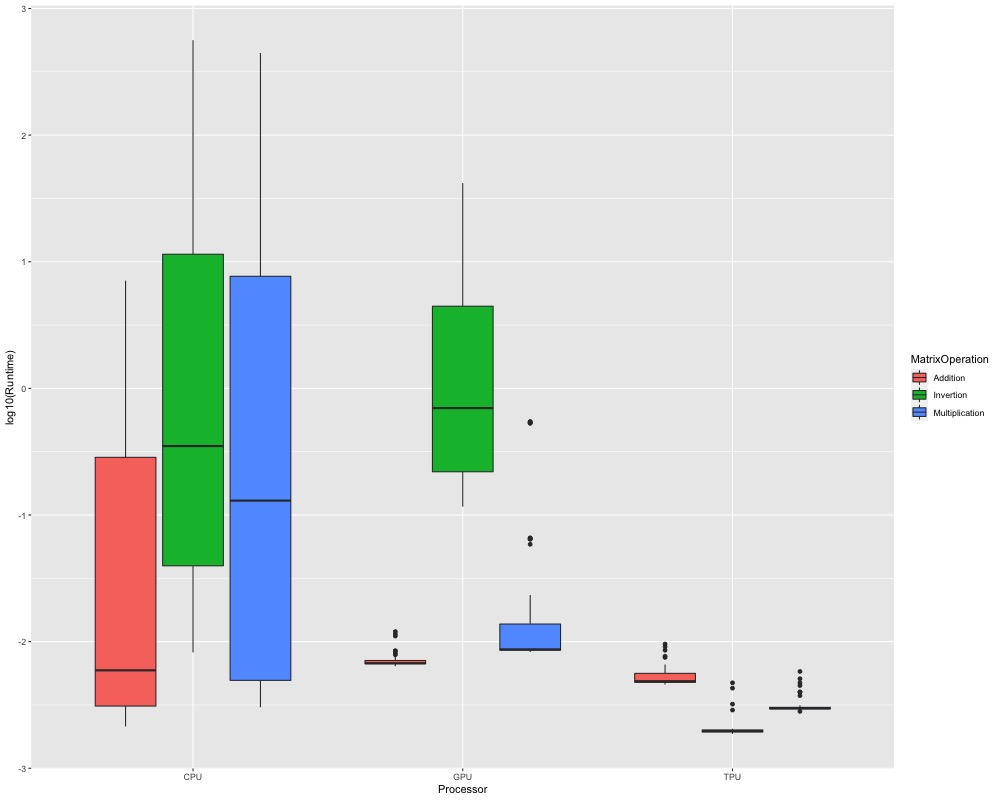
\includegraphics[width=0.9\linewidth]{../figs/overview} \end{center}

\hypertarget{jingbin-cao-part-i}{%
\section{Jingbin Cao Part I}\label{jingbin-cao-part-i}}

Research different Matrix Sizes One Way Anova for different matrix sized
for each pair of processor and matrix operation:
\(\mu_1 = Matrix_{Size}=160\) \(\mu_2 = Matrix_{Size}=320\)
\(\mu_3 = Matrix_{Size}=640\) \(\mu_4 = Matrix_{Size}=1280\)

\hypertarget{getting-data}{%
\subsection{Getting Data}\label{getting-data}}

\begin{Shaded}
\begin{Highlighting}[]
\NormalTok{cpu\_add \textless{}{-}}\StringTok{ }\NormalTok{data[data}\OperatorTok{$}\NormalTok{Processor }\OperatorTok{==}\StringTok{ "CPU"} \OperatorTok{\&}\StringTok{ }\NormalTok{data}\OperatorTok{$}\NormalTok{MatrixOperation}\OperatorTok{==}\StringTok{"Addition"} \OperatorTok{\&}\StringTok{ }\NormalTok{data}\OperatorTok{$}\NormalTok{MatrixSize }\OperatorTok{\textgreater{}=}\StringTok{ }\DecValTok{160}\NormalTok{,]}
\NormalTok{cpu\_mult \textless{}{-}}\StringTok{ }\NormalTok{data[data}\OperatorTok{$}\NormalTok{Processor }\OperatorTok{==}\StringTok{ "CPU"} \OperatorTok{\&}\StringTok{ }\NormalTok{data}\OperatorTok{$}\NormalTok{MatrixOperation}\OperatorTok{==}\StringTok{"Multiplication"} \OperatorTok{\&}\StringTok{ }\NormalTok{data}\OperatorTok{$}\NormalTok{MatrixSize }\OperatorTok{\textgreater{}=}\StringTok{ }\DecValTok{160}\NormalTok{,]}
\NormalTok{cpu\_inv \textless{}{-}}\StringTok{ }\NormalTok{data[data}\OperatorTok{$}\NormalTok{Processor }\OperatorTok{==}\StringTok{ "CPU"} \OperatorTok{\&}\StringTok{ }\NormalTok{data}\OperatorTok{$}\NormalTok{MatrixOperation}\OperatorTok{==}\StringTok{"Inversion"} \OperatorTok{\&}\StringTok{ }\NormalTok{data}\OperatorTok{$}\NormalTok{MatrixSize }\OperatorTok{\textgreater{}=}\StringTok{ }\DecValTok{160}\NormalTok{,]}
\NormalTok{gpu\_add \textless{}{-}}\StringTok{ }\NormalTok{data[data}\OperatorTok{$}\NormalTok{Processor }\OperatorTok{==}\StringTok{ "GPU"} \OperatorTok{\&}\StringTok{ }\NormalTok{data}\OperatorTok{$}\NormalTok{MatrixOperation}\OperatorTok{==}\StringTok{"Addition"} \OperatorTok{\&}\StringTok{ }\NormalTok{data}\OperatorTok{$}\NormalTok{MatrixSize }\OperatorTok{\textgreater{}=}\StringTok{ }\DecValTok{160}\NormalTok{,]}
\NormalTok{gpu\_mult \textless{}{-}}\StringTok{ }\NormalTok{data[data}\OperatorTok{$}\NormalTok{Processor }\OperatorTok{==}\StringTok{ "GPU"} \OperatorTok{\&}\StringTok{ }\NormalTok{data}\OperatorTok{$}\NormalTok{MatrixOperation}\OperatorTok{==}\StringTok{"Multiplication"} \OperatorTok{\&}\StringTok{ }\NormalTok{data}\OperatorTok{$}\NormalTok{MatrixSize }\OperatorTok{\textgreater{}=}\StringTok{ }\DecValTok{160}\NormalTok{,]}
\NormalTok{gpu\_inv \textless{}{-}}\StringTok{ }\NormalTok{data[data}\OperatorTok{$}\NormalTok{Processor }\OperatorTok{==}\StringTok{ "GPU"} \OperatorTok{\&}\StringTok{ }\NormalTok{data}\OperatorTok{$}\NormalTok{MatrixOperation}\OperatorTok{==}\StringTok{"Inversion"} \OperatorTok{\&}\StringTok{ }\NormalTok{data}\OperatorTok{$}\NormalTok{MatrixSize }\OperatorTok{\textgreater{}=}\StringTok{ }\DecValTok{160}\NormalTok{,]}
\NormalTok{tpu\_add \textless{}{-}}\StringTok{ }\NormalTok{data[data}\OperatorTok{$}\NormalTok{Processor }\OperatorTok{==}\StringTok{ "TPU"} \OperatorTok{\&}\StringTok{ }\NormalTok{data}\OperatorTok{$}\NormalTok{MatrixOperation}\OperatorTok{==}\StringTok{"Addition"} \OperatorTok{\&}\StringTok{ }\NormalTok{data}\OperatorTok{$}\NormalTok{MatrixSize }\OperatorTok{\textgreater{}=}\StringTok{ }\DecValTok{160}\NormalTok{,]}
\NormalTok{tpu\_mult \textless{}{-}}\StringTok{ }\NormalTok{data[data}\OperatorTok{$}\NormalTok{Processor }\OperatorTok{==}\StringTok{ "TPU"} \OperatorTok{\&}\StringTok{ }\NormalTok{data}\OperatorTok{$}\NormalTok{MatrixOperation}\OperatorTok{==}\StringTok{"Multiplication"} \OperatorTok{\&}\StringTok{ }\NormalTok{data}\OperatorTok{$}\NormalTok{MatrixSize }\OperatorTok{\textgreater{}=}\StringTok{ }\DecValTok{160}\NormalTok{,]}
\NormalTok{tpu\_inv \textless{}{-}}\StringTok{ }\NormalTok{data[data}\OperatorTok{$}\NormalTok{Processor }\OperatorTok{==}\StringTok{ "TPU"} \OperatorTok{\&}\StringTok{ }\NormalTok{data}\OperatorTok{$}\NormalTok{MatrixOperation}\OperatorTok{==}\StringTok{"Inversion"} \OperatorTok{\&}\StringTok{ }\NormalTok{data}\OperatorTok{$}\NormalTok{MatrixSize }\OperatorTok{\textgreater{}=}\StringTok{ }\DecValTok{160}\NormalTok{,]}
\end{Highlighting}
\end{Shaded}

\hypertarget{anovas}{%
\subsection{Anovas}\label{anovas}}

\begin{Shaded}
\begin{Highlighting}[]
\KeywordTok{summary}\NormalTok{(mod\_cpu\_add \textless{}{-}}\StringTok{ }\KeywordTok{aov}\NormalTok{(}\KeywordTok{log10}\NormalTok{(Runtime) }\OperatorTok{\textasciitilde{}}\StringTok{ }\KeywordTok{as.factor}\NormalTok{(MatrixSize), }\DataTypeTok{data=}\NormalTok{cpu\_add))}
\end{Highlighting}
\end{Shaded}

\begin{verbatim}
##                       Df Sum Sq Mean Sq F value Pr(>F)    
## as.factor(MatrixSize)  3 15.478   5.159   76040 <2e-16 ***
## Residuals             16  0.001   0.000                   
## ---
## Signif. codes:  0 '***' 0.001 '**' 0.01 '*' 0.05 '.' 0.1 ' ' 1
\end{verbatim}

\begin{Shaded}
\begin{Highlighting}[]
\KeywordTok{summary}\NormalTok{(mod\_cpu\_mult \textless{}{-}}\StringTok{ }\KeywordTok{aov}\NormalTok{(}\KeywordTok{log10}\NormalTok{(Runtime) }\OperatorTok{\textasciitilde{}}\StringTok{ }\KeywordTok{as.factor}\NormalTok{(MatrixSize), }\DataTypeTok{data=}\NormalTok{cpu\_mult))}
\end{Highlighting}
\end{Shaded}

\begin{verbatim}
##                       Df Sum Sq Mean Sq F value Pr(>F)    
## as.factor(MatrixSize)  3  19.53   6.511  393855 <2e-16 ***
## Residuals             16   0.00   0.000                   
## ---
## Signif. codes:  0 '***' 0.001 '**' 0.01 '*' 0.05 '.' 0.1 ' ' 1
\end{verbatim}

\begin{Shaded}
\begin{Highlighting}[]
\KeywordTok{summary}\NormalTok{(mod\_cpu\_inv \textless{}{-}}\StringTok{ }\KeywordTok{aov}\NormalTok{(}\KeywordTok{log10}\NormalTok{(Runtime) }\OperatorTok{\textasciitilde{}}\StringTok{ }\KeywordTok{as.factor}\NormalTok{(MatrixSize), }\DataTypeTok{data=}\NormalTok{cpu\_inv))}
\end{Highlighting}
\end{Shaded}

\begin{verbatim}
##                       Df Sum Sq Mean Sq F value Pr(>F)    
## as.factor(MatrixSize)  3  15.67   5.223  653718 <2e-16 ***
## Residuals             16   0.00   0.000                   
## ---
## Signif. codes:  0 '***' 0.001 '**' 0.01 '*' 0.05 '.' 0.1 ' ' 1
\end{verbatim}

\begin{Shaded}
\begin{Highlighting}[]
\KeywordTok{summary}\NormalTok{(mod\_gpu\_add \textless{}{-}}\StringTok{ }\KeywordTok{aov}\NormalTok{(}\KeywordTok{log10}\NormalTok{(Runtime) }\OperatorTok{\textasciitilde{}}\StringTok{ }\KeywordTok{as.factor}\NormalTok{(MatrixSize), }\DataTypeTok{data=}\NormalTok{gpu\_add))}
\end{Highlighting}
\end{Shaded}

\begin{verbatim}
##                       Df Sum Sq Mean Sq F value Pr(>F)    
## as.factor(MatrixSize)  3 2.6297  0.8766   10205 <2e-16 ***
## Residuals             16 0.0014  0.0001                   
## ---
## Signif. codes:  0 '***' 0.001 '**' 0.01 '*' 0.05 '.' 0.1 ' ' 1
\end{verbatim}

\begin{Shaded}
\begin{Highlighting}[]
\KeywordTok{summary}\NormalTok{(mod\_gpu\_mult \textless{}{-}}\StringTok{ }\KeywordTok{aov}\NormalTok{(}\KeywordTok{log10}\NormalTok{(Runtime) }\OperatorTok{\textasciitilde{}}\StringTok{ }\KeywordTok{as.factor}\NormalTok{(MatrixSize), }\DataTypeTok{data=}\NormalTok{gpu\_mult))}
\end{Highlighting}
\end{Shaded}

\begin{verbatim}
##                       Df Sum Sq Mean Sq F value Pr(>F)    
## as.factor(MatrixSize)  3 12.328   4.109   34853 <2e-16 ***
## Residuals             16  0.002   0.000                   
## ---
## Signif. codes:  0 '***' 0.001 '**' 0.01 '*' 0.05 '.' 0.1 ' ' 1
\end{verbatim}

\begin{Shaded}
\begin{Highlighting}[]
\KeywordTok{summary}\NormalTok{(mod\_gpu\_inv \textless{}{-}}\StringTok{ }\KeywordTok{aov}\NormalTok{(}\KeywordTok{log10}\NormalTok{(Runtime) }\OperatorTok{\textasciitilde{}}\StringTok{ }\KeywordTok{as.factor}\NormalTok{(MatrixSize), }\DataTypeTok{data=}\NormalTok{gpu\_inv))}
\end{Highlighting}
\end{Shaded}

\begin{verbatim}
##                       Df Sum Sq Mean Sq F value Pr(>F)    
## as.factor(MatrixSize)  3  4.083   1.361 4518902 <2e-16 ***
## Residuals             16  0.000   0.000                   
## ---
## Signif. codes:  0 '***' 0.001 '**' 0.01 '*' 0.05 '.' 0.1 ' ' 1
\end{verbatim}

\begin{Shaded}
\begin{Highlighting}[]
\KeywordTok{summary}\NormalTok{(mod\_tpu\_add \textless{}{-}}\StringTok{ }\KeywordTok{aov}\NormalTok{(}\KeywordTok{log10}\NormalTok{(Runtime) }\OperatorTok{\textasciitilde{}}\StringTok{ }\KeywordTok{as.factor}\NormalTok{(MatrixSize), }\DataTypeTok{data=}\NormalTok{tpu\_add))}
\end{Highlighting}
\end{Shaded}

\begin{verbatim}
##                       Df   Sum Sq  Mean Sq F value Pr(>F)
## as.factor(MatrixSize)  3 0.003245 0.001081   0.849  0.487
## Residuals             16 0.020376 0.001273
\end{verbatim}

\begin{Shaded}
\begin{Highlighting}[]
\KeywordTok{summary}\NormalTok{(mod\_tpu\_mult \textless{}{-}}\StringTok{ }\KeywordTok{aov}\NormalTok{(}\KeywordTok{log10}\NormalTok{(Runtime) }\OperatorTok{\textasciitilde{}}\StringTok{ }\KeywordTok{as.factor}\NormalTok{(MatrixSize), }\DataTypeTok{data=}\NormalTok{tpu\_mult))}
\end{Highlighting}
\end{Shaded}

\begin{verbatim}
##                       Df  Sum Sq  Mean Sq F value Pr(>F)
## as.factor(MatrixSize)  3 0.00678 0.002259   0.707  0.562
## Residuals             16 0.05116 0.003197
\end{verbatim}

\begin{Shaded}
\begin{Highlighting}[]
\KeywordTok{summary}\NormalTok{(mod\_tpu\_inv \textless{}{-}}\StringTok{ }\KeywordTok{aov}\NormalTok{(}\KeywordTok{log10}\NormalTok{(Runtime) }\OperatorTok{\textasciitilde{}}\StringTok{ }\KeywordTok{as.factor}\NormalTok{(MatrixSize), }\DataTypeTok{data=}\NormalTok{tpu\_inv))}
\end{Highlighting}
\end{Shaded}

\begin{verbatim}
##                       Df  Sum Sq  Mean Sq F value Pr(>F)
## as.factor(MatrixSize)  3 0.00667 0.002224   0.936  0.446
## Residuals             16 0.03801 0.002376
\end{verbatim}

\begin{Shaded}
\begin{Highlighting}[]
\CommentTok{\# From the tables, we can see that only TPU \& Multiplication and TPU \& Inversion do not have Matrix Size effect, but other nine pairs do have Matrix Size effects.}
\CommentTok{\# plot(aov(Runtime \textasciitilde{} as.factor(MatrixSize), data=tpu\_mult))}
\CommentTok{\# plot(aov(Runtime \textasciitilde{} as.factor(MatrixSize), data=tpu\_inv))}
\end{Highlighting}
\end{Shaded}

\hypertarget{confidence-interval-for-lms}{%
\subsubsection{Confidence Interval for
LMs}\label{confidence-interval-for-lms}}

\begin{Shaded}
\begin{Highlighting}[]
\KeywordTok{round}\NormalTok{(}\DataTypeTok{digits=}\DecValTok{4}\NormalTok{,}\KeywordTok{confint}\NormalTok{(mod\_cpu\_add))}
\end{Highlighting}
\end{Shaded}

\begin{verbatim}
##                             2.5 %  97.5 %
## (Intercept)               -1.1994 -1.1838
## as.factor(MatrixSize)320   1.0339  1.0560
## as.factor(MatrixSize)640   1.6346  1.6567
## as.factor(MatrixSize)1280  2.3952  2.4173
\end{verbatim}

\begin{Shaded}
\begin{Highlighting}[]
\KeywordTok{round}\NormalTok{(}\DataTypeTok{digits=}\DecValTok{4}\NormalTok{,}\KeywordTok{confint}\NormalTok{(mod\_cpu\_mult))}
\end{Highlighting}
\end{Shaded}

\begin{verbatim}
##                            2.5 % 97.5 %
## (Intercept)               0.1445 0.1522
## as.factor(MatrixSize)320  0.9245 0.9354
## as.factor(MatrixSize)640  1.7674 1.7783
## as.factor(MatrixSize)1280 2.6596 2.6705
\end{verbatim}

\begin{Shaded}
\begin{Highlighting}[]
\KeywordTok{round}\NormalTok{(}\DataTypeTok{digits=}\DecValTok{4}\NormalTok{,}\KeywordTok{confint}\NormalTok{(mod\_cpu\_inv))}
\end{Highlighting}
\end{Shaded}

\begin{verbatim}
##                            2.5 % 97.5 %
## (Intercept)               0.5928 0.5982
## as.factor(MatrixSize)320  0.6918 0.6994
## as.factor(MatrixSize)640  1.5130 1.5206
## as.factor(MatrixSize)1280 2.3589 2.3664
\end{verbatim}

\begin{Shaded}
\begin{Highlighting}[]
\KeywordTok{round}\NormalTok{(}\KeywordTok{confint}\NormalTok{(mod\_gpu\_add),}\DecValTok{4}\NormalTok{)}
\end{Highlighting}
\end{Shaded}

\begin{verbatim}
##                             2.5 %  97.5 %
## (Intercept)               -1.1665 -1.1489
## as.factor(MatrixSize)320  -0.0066  0.0183
## as.factor(MatrixSize)640   0.0865  0.1114
## as.factor(MatrixSize)1280  0.8550  0.8798
\end{verbatim}

\begin{Shaded}
\begin{Highlighting}[]
\KeywordTok{round}\NormalTok{(}\DataTypeTok{digits=}\DecValTok{4}\NormalTok{,}\KeywordTok{confint}\NormalTok{(mod\_gpu\_mult))}
\end{Highlighting}
\end{Shaded}

\begin{verbatim}
##                             2.5 %  97.5 %
## (Intercept)               -1.0610 -1.0404
## as.factor(MatrixSize)320   0.3907  0.4198
## as.factor(MatrixSize)640   1.1183  1.1474
## as.factor(MatrixSize)1280  2.0502  2.0793
\end{verbatim}

\begin{Shaded}
\begin{Highlighting}[]
\KeywordTok{round}\NormalTok{(}\DataTypeTok{digits=}\DecValTok{4}\NormalTok{,}\KeywordTok{confint}\NormalTok{(mod\_gpu\_inv))}
\end{Highlighting}
\end{Shaded}

\begin{verbatim}
##                            2.5 % 97.5 %
## (Intercept)               0.8389 0.8400
## as.factor(MatrixSize)320  0.4203 0.4218
## as.factor(MatrixSize)640  0.8101 0.8116
## as.factor(MatrixSize)1280 1.2162 1.2177
\end{verbatim}

\hypertarget{zhanhao-zhang-part-i}{%
\section{Zhanhao Zhang Part I}\label{zhanhao-zhang-part-i}}

\hypertarget{interaction-plots}{%
\subsection{Interaction Plots}\label{interaction-plots}}

\begin{Shaded}
\begin{Highlighting}[]
\CommentTok{\#ggplot(data = data, aes(x = Processor, y = log10(Runtime))) +}
 \CommentTok{\# geom\_boxplot(aes(fill = MatrixOperation))}
\ControlFlowTok{for}\NormalTok{(operation }\ControlFlowTok{in} \KeywordTok{unique}\NormalTok{(data}\OperatorTok{$}\NormalTok{MatrixOperation))\{}
  \CommentTok{\#png(paste0("../figs/", operation, ".png"), width = 500, height = 500)}
\NormalTok{  p \textless{}{-}}\StringTok{ }\NormalTok{data }\OperatorTok{\%\textgreater{}\%}
\StringTok{    }\NormalTok{dplyr}\OperatorTok{::}\KeywordTok{filter}\NormalTok{(MatrixOperation }\OperatorTok{==}\StringTok{ }\NormalTok{operation) }\OperatorTok{\%\textgreater{}\%}
\StringTok{    }\KeywordTok{group\_by}\NormalTok{(MatrixSize, MatrixOperation, Processor) }\OperatorTok{\%\textgreater{}\%}
\StringTok{    }\NormalTok{dplyr}\OperatorTok{::}\KeywordTok{summarize}\NormalTok{(}\DataTypeTok{Runtime =} \KeywordTok{mean}\NormalTok{(Runtime)) }\OperatorTok{\%\textgreater{}\%}
\StringTok{    }\KeywordTok{ggplot}\NormalTok{(}\KeywordTok{aes}\NormalTok{(}\DataTypeTok{x =}\NormalTok{ Processor, }\DataTypeTok{y =}\NormalTok{ Runtime)) }\OperatorTok{+}
\StringTok{    }\CommentTok{\#geom\_boxplot(aes(fill = as.factor(MatrixSize))) +}
\StringTok{    }\KeywordTok{geom\_bar}\NormalTok{(}\KeywordTok{aes}\NormalTok{(}\DataTypeTok{fill =} \KeywordTok{as.factor}\NormalTok{(MatrixSize)), }\DataTypeTok{stat =} \StringTok{"identity"}\NormalTok{,}
             \DataTypeTok{position =} \StringTok{"dodge"}\NormalTok{) }\OperatorTok{+}
\StringTok{    }\KeywordTok{scale\_y\_log10}\NormalTok{() }\OperatorTok{+}
\StringTok{    }\KeywordTok{ggtitle}\NormalTok{(}\KeywordTok{paste0}\NormalTok{(}\StringTok{"Matrix Operation: "}\NormalTok{, operation)) }\OperatorTok{+}
\StringTok{    }\CommentTok{\#facet\_wrap( \textasciitilde{} MatrixOperation, scales = "free", nrow = 1) +}
\StringTok{    }\KeywordTok{guides}\NormalTok{(}\DataTypeTok{fill=}\KeywordTok{guide\_legend}\NormalTok{(}\DataTypeTok{title =} \StringTok{"Matrix Size"}\NormalTok{))}
  \KeywordTok{print}\NormalTok{(p)}
  \CommentTok{\#dev.off()}
\NormalTok{\}}
\end{Highlighting}
\end{Shaded}

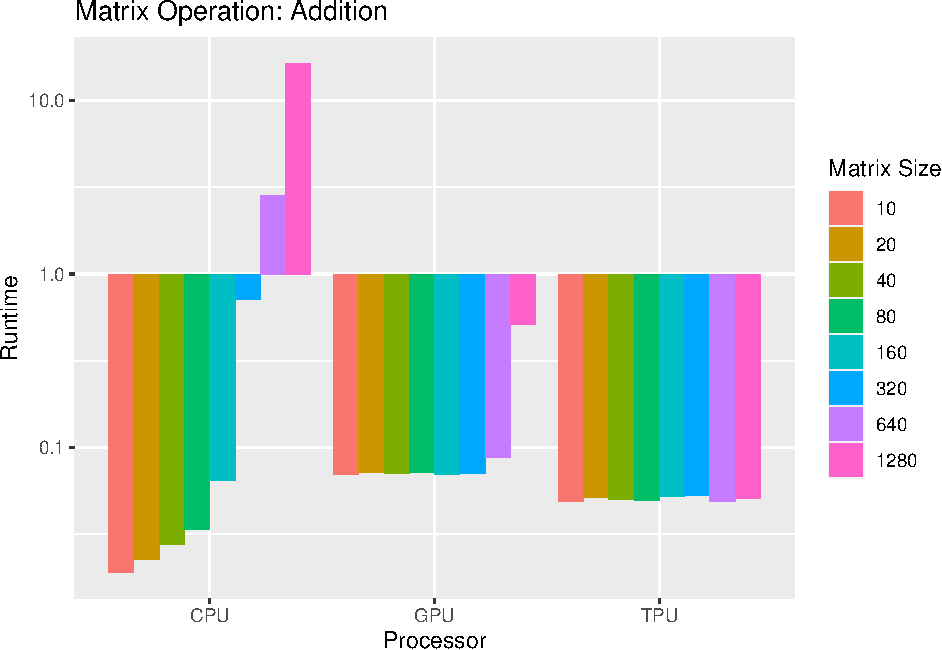
\includegraphics{main_files/figure-latex/unnamed-chunk-7-1.pdf}
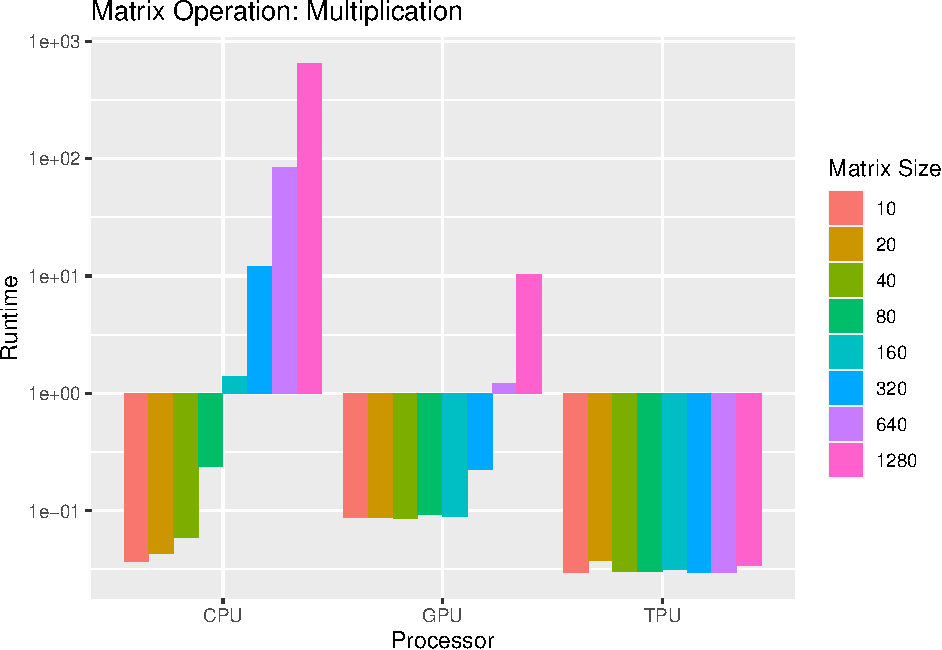
\includegraphics{main_files/figure-latex/unnamed-chunk-7-2.pdf}
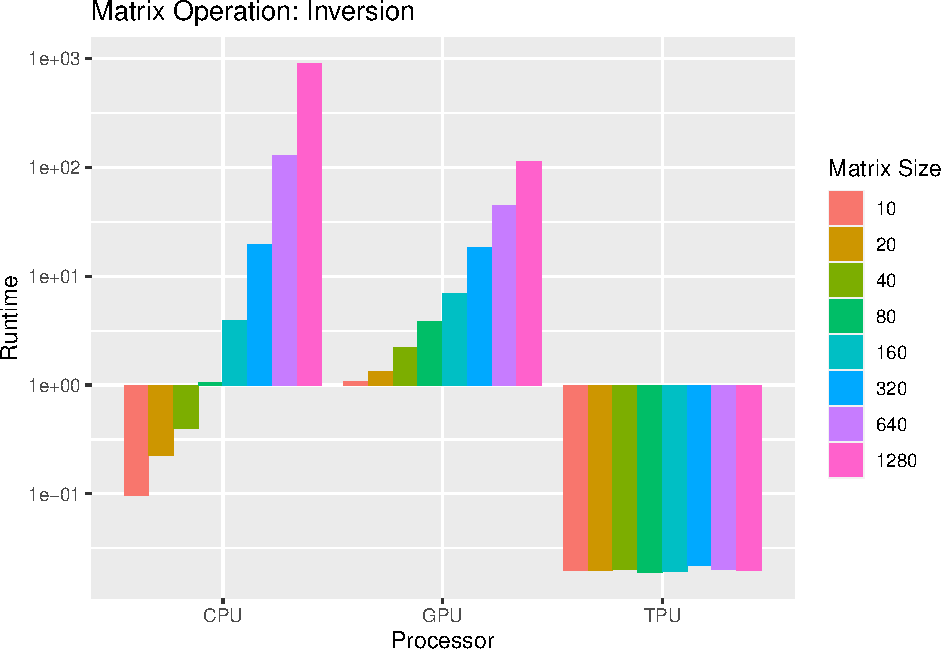
\includegraphics{main_files/figure-latex/unnamed-chunk-7-3.pdf}

\begin{Shaded}
\begin{Highlighting}[]
\ControlFlowTok{for}\NormalTok{(size }\ControlFlowTok{in} \KeywordTok{unique}\NormalTok{(data}\OperatorTok{$}\NormalTok{MatrixSize))\{}
\NormalTok{  p \textless{}{-}}\StringTok{ }\NormalTok{data }\OperatorTok{\%\textgreater{}\%}
\StringTok{    }\NormalTok{dplyr}\OperatorTok{::}\KeywordTok{filter}\NormalTok{(MatrixSize }\OperatorTok{==}\StringTok{ }\NormalTok{size) }\OperatorTok{\%\textgreater{}\%}
\StringTok{    }\KeywordTok{group\_by}\NormalTok{(MatrixSize, MatrixOperation, Processor) }\OperatorTok{\%\textgreater{}\%}
\StringTok{    }\KeywordTok{summarize}\NormalTok{(}\DataTypeTok{Runtime =} \KeywordTok{mean}\NormalTok{(Runtime)) }\OperatorTok{\%\textgreater{}\%}
\StringTok{    }\KeywordTok{ggplot}\NormalTok{(}\KeywordTok{aes}\NormalTok{(}\DataTypeTok{x =}\NormalTok{ Processor, }\DataTypeTok{y =}\NormalTok{ Runtime)) }\OperatorTok{+}
\StringTok{    }\CommentTok{\#geom\_boxplot(aes(fill = as.factor(MatrixOperation))) +}
\StringTok{    }\KeywordTok{geom\_bar}\NormalTok{(}\KeywordTok{aes}\NormalTok{(}\DataTypeTok{fill =} \KeywordTok{as.factor}\NormalTok{(MatrixOperation)), }\DataTypeTok{position =} \StringTok{"dodge"}\NormalTok{,}
             \DataTypeTok{stat =} \StringTok{"identity"}\NormalTok{) }\OperatorTok{+}
\StringTok{    }\KeywordTok{scale\_y\_log10}\NormalTok{() }\OperatorTok{+}
\StringTok{    }\KeywordTok{ggtitle}\NormalTok{(}\KeywordTok{paste0}\NormalTok{(}\StringTok{"Matrix Size: "}\NormalTok{, size)) }\OperatorTok{+}
\StringTok{    }\CommentTok{\#facet\_wrap( \textasciitilde{} MatrixOperation, scales = "free", nrow = 1) +}
\StringTok{    }\KeywordTok{guides}\NormalTok{(}\DataTypeTok{fill=}\KeywordTok{guide\_legend}\NormalTok{(}\DataTypeTok{title =} \StringTok{"Matrix Operation"}\NormalTok{))}
  \KeywordTok{print}\NormalTok{(p)}
\NormalTok{\}}
\end{Highlighting}
\end{Shaded}

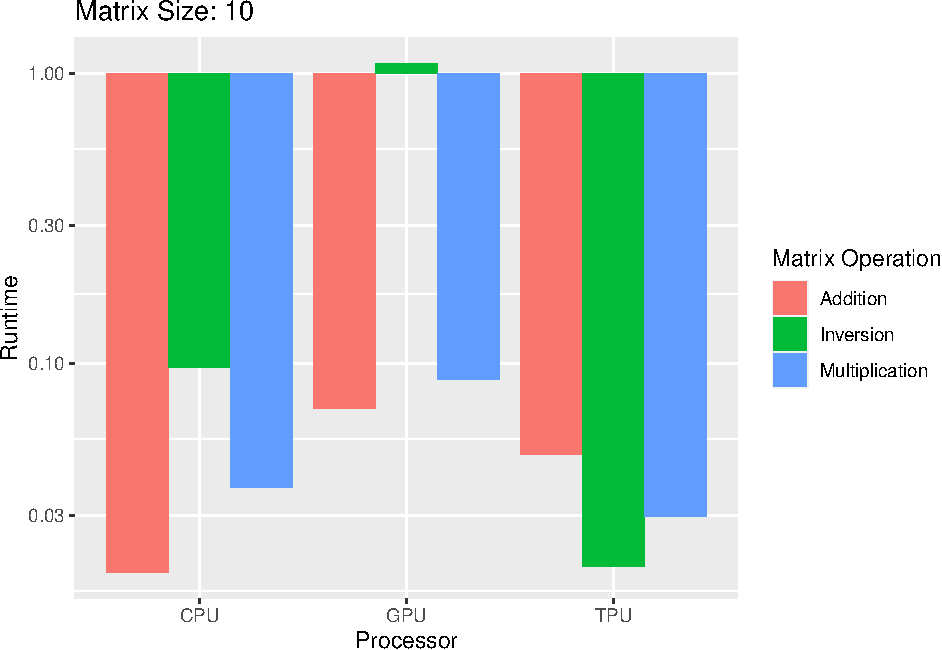
\includegraphics{main_files/figure-latex/unnamed-chunk-8-1.pdf}
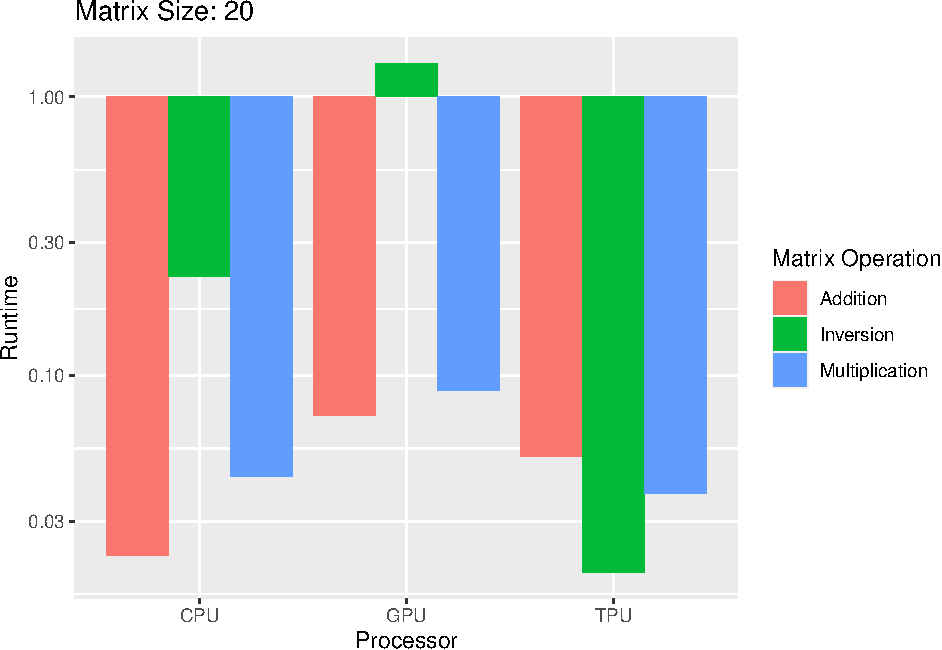
\includegraphics{main_files/figure-latex/unnamed-chunk-8-2.pdf}
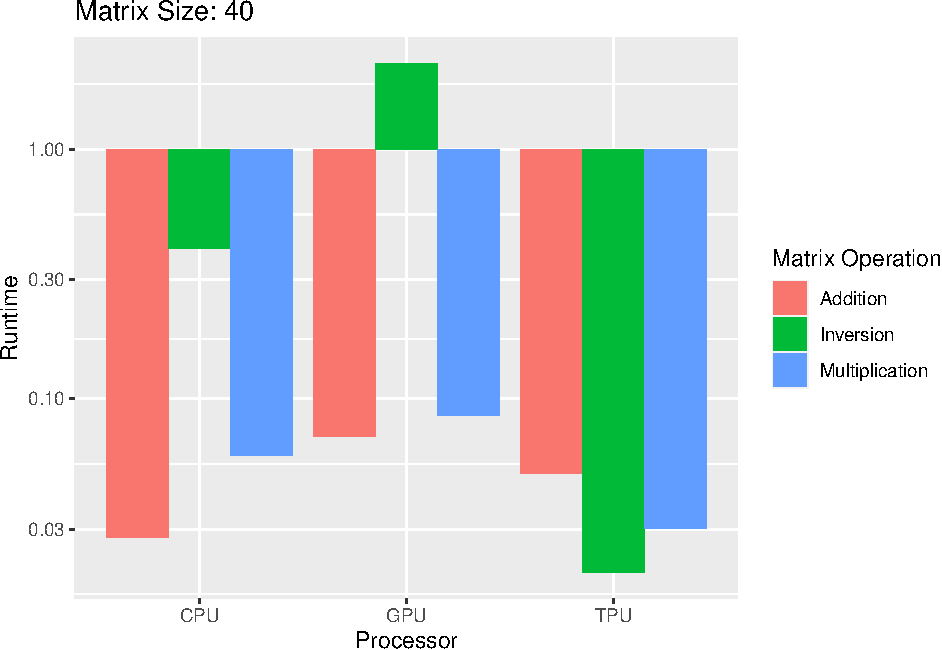
\includegraphics{main_files/figure-latex/unnamed-chunk-8-3.pdf}
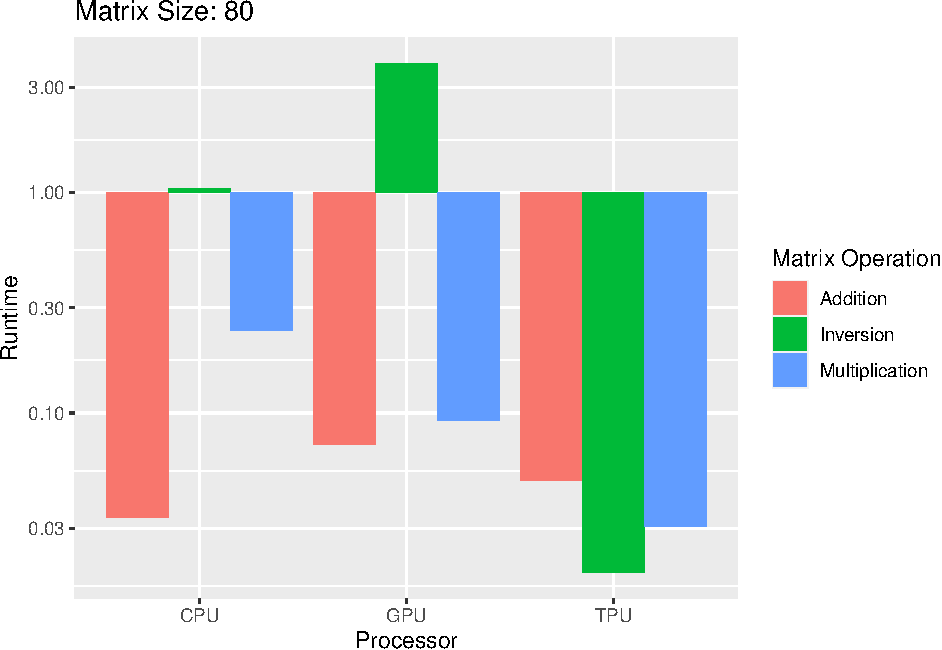
\includegraphics{main_files/figure-latex/unnamed-chunk-8-4.pdf}
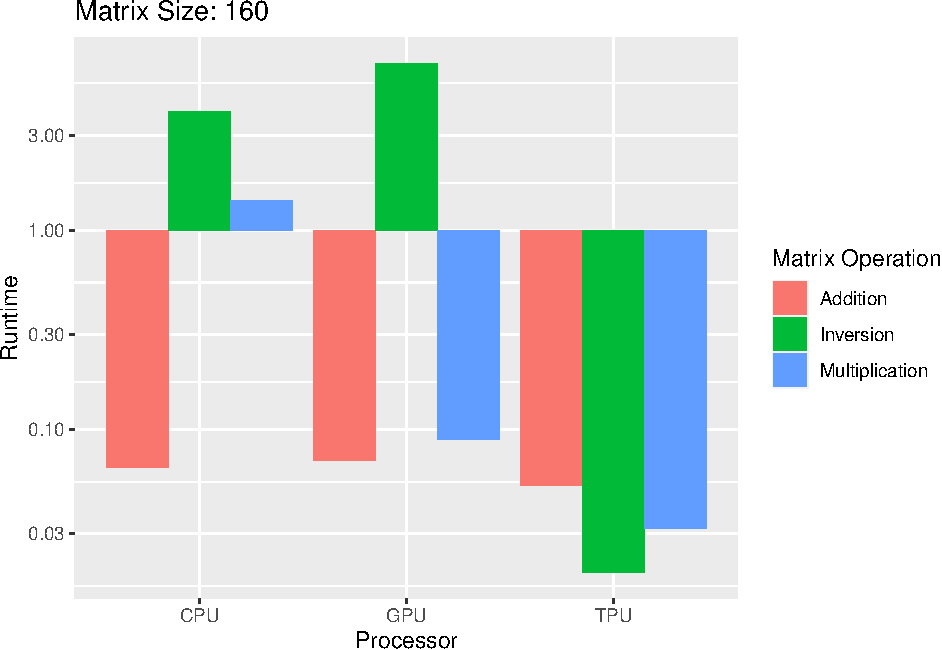
\includegraphics{main_files/figure-latex/unnamed-chunk-8-5.pdf}
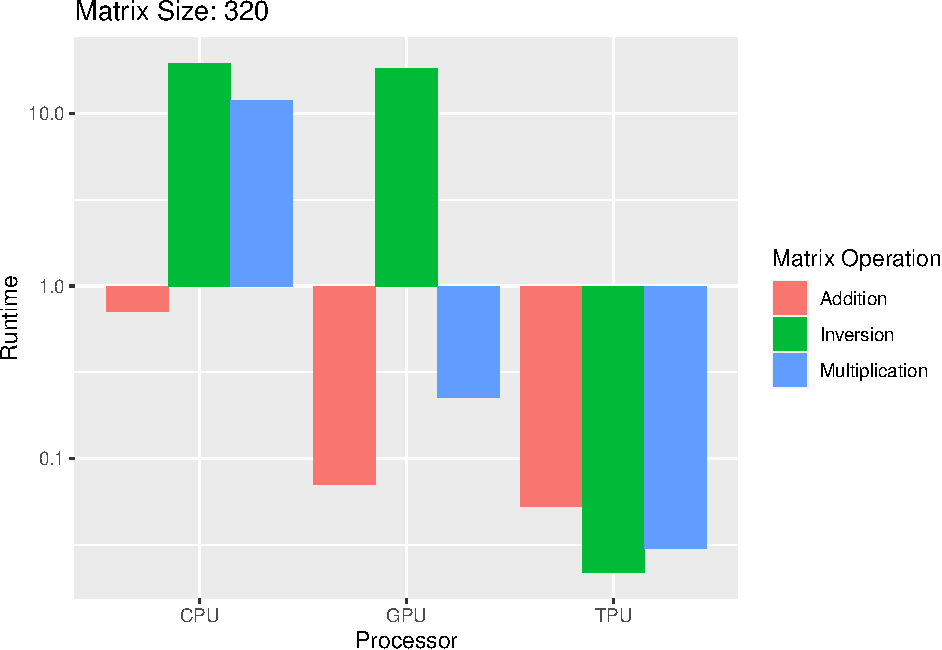
\includegraphics{main_files/figure-latex/unnamed-chunk-8-6.pdf}
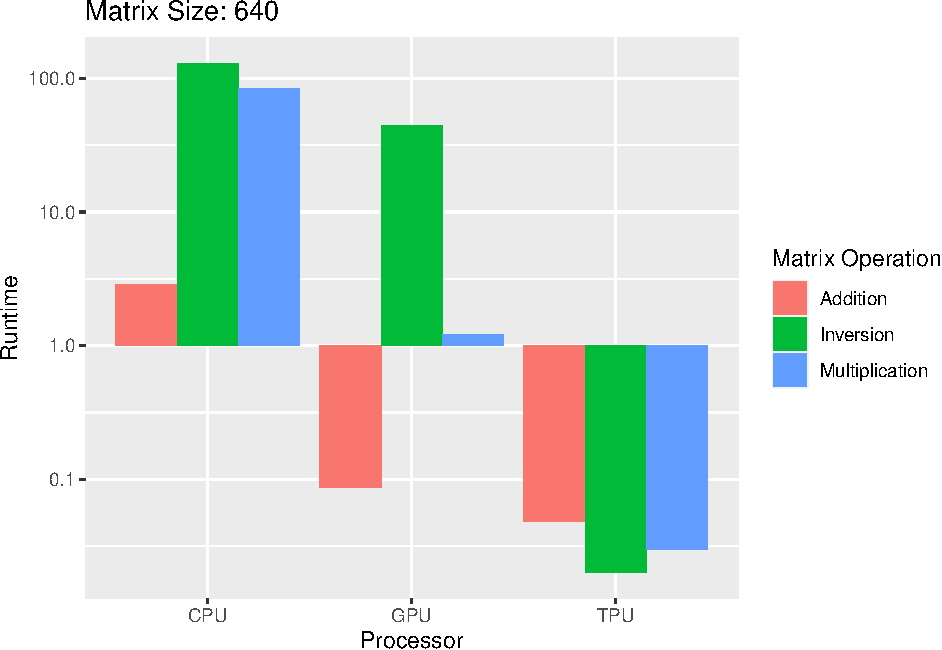
\includegraphics{main_files/figure-latex/unnamed-chunk-8-7.pdf}
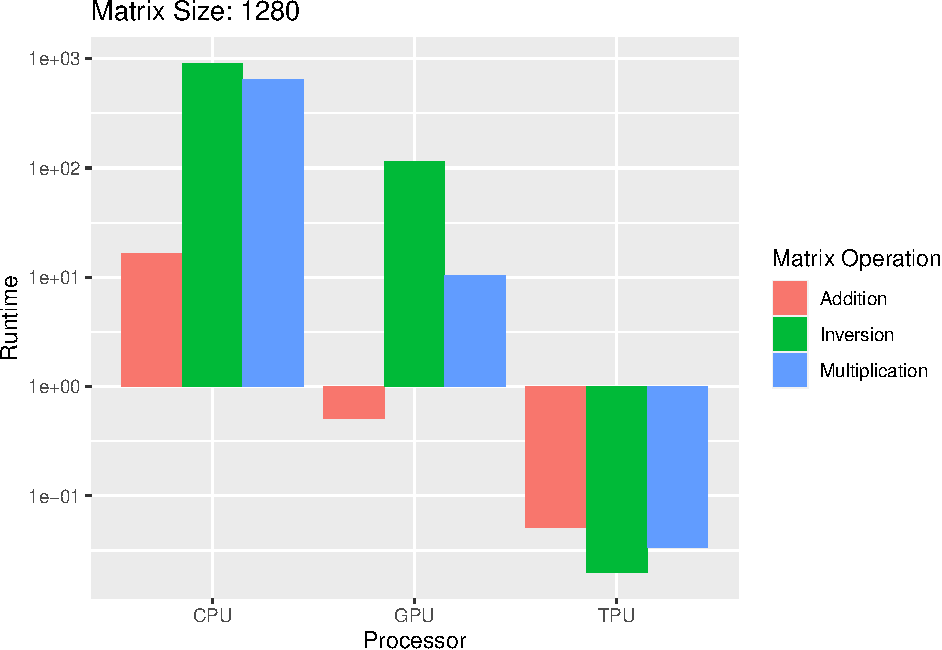
\includegraphics{main_files/figure-latex/unnamed-chunk-8-8.pdf}

\begin{Shaded}
\begin{Highlighting}[]
\ControlFlowTok{for}\NormalTok{(size }\ControlFlowTok{in} \KeywordTok{unique}\NormalTok{(data}\OperatorTok{$}\NormalTok{MatrixSize))\{}
\NormalTok{  p \textless{}{-}}\StringTok{ }\NormalTok{data }\OperatorTok{\%\textgreater{}\%}
\StringTok{    }\NormalTok{dplyr}\OperatorTok{::}\KeywordTok{filter}\NormalTok{(MatrixSize }\OperatorTok{==}\StringTok{ }\NormalTok{size) }\OperatorTok{\%\textgreater{}\%}
\StringTok{    }\KeywordTok{group\_by}\NormalTok{(MatrixSize, MatrixOperation, Processor) }\OperatorTok{\%\textgreater{}\%}
\StringTok{    }\KeywordTok{summarize}\NormalTok{(}\DataTypeTok{Runtime =} \KeywordTok{mean}\NormalTok{(Runtime)) }\OperatorTok{\%\textgreater{}\%}
\StringTok{    }\KeywordTok{ggplot}\NormalTok{(}\KeywordTok{aes}\NormalTok{(}\DataTypeTok{x =}\NormalTok{ MatrixOperation, }\DataTypeTok{y =}\NormalTok{ Runtime)) }\OperatorTok{+}
\StringTok{    }\CommentTok{\#geom\_boxplot(aes(fill = as.factor(Processor))) +}
\StringTok{    }\KeywordTok{geom\_bar}\NormalTok{(}\KeywordTok{aes}\NormalTok{(}\DataTypeTok{fill =} \KeywordTok{as.factor}\NormalTok{(Processor)), }\DataTypeTok{position =} \StringTok{"dodge"}\NormalTok{, }
             \DataTypeTok{stat =} \StringTok{"identity"}\NormalTok{) }\OperatorTok{+}
\StringTok{    }\KeywordTok{scale\_y\_log10}\NormalTok{() }\OperatorTok{+}
\StringTok{    }\KeywordTok{ggtitle}\NormalTok{(}\KeywordTok{paste0}\NormalTok{(}\StringTok{"Matrix Size: "}\NormalTok{, size)) }\OperatorTok{+}
\StringTok{    }\CommentTok{\#facet\_wrap( \textasciitilde{} MatrixOperation, scales = "free", nrow = 1) +}
\StringTok{    }\KeywordTok{guides}\NormalTok{(}\DataTypeTok{fill=}\KeywordTok{guide\_legend}\NormalTok{(}\DataTypeTok{title =} \StringTok{"Processor"}\NormalTok{))}
  \KeywordTok{print}\NormalTok{(p)}
\NormalTok{\}}
\end{Highlighting}
\end{Shaded}

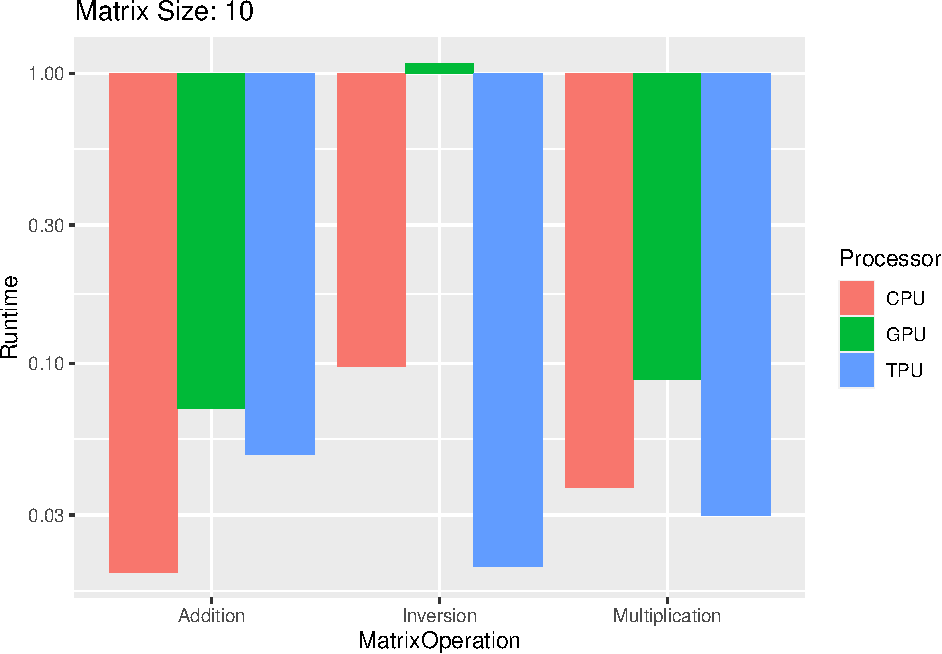
\includegraphics{main_files/figure-latex/unnamed-chunk-9-1.pdf}
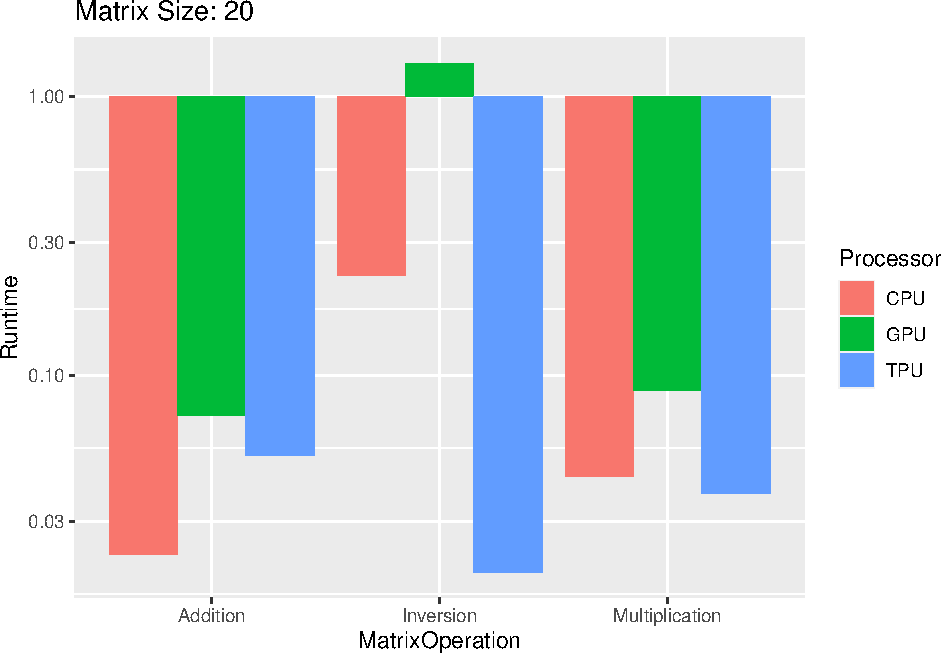
\includegraphics{main_files/figure-latex/unnamed-chunk-9-2.pdf}
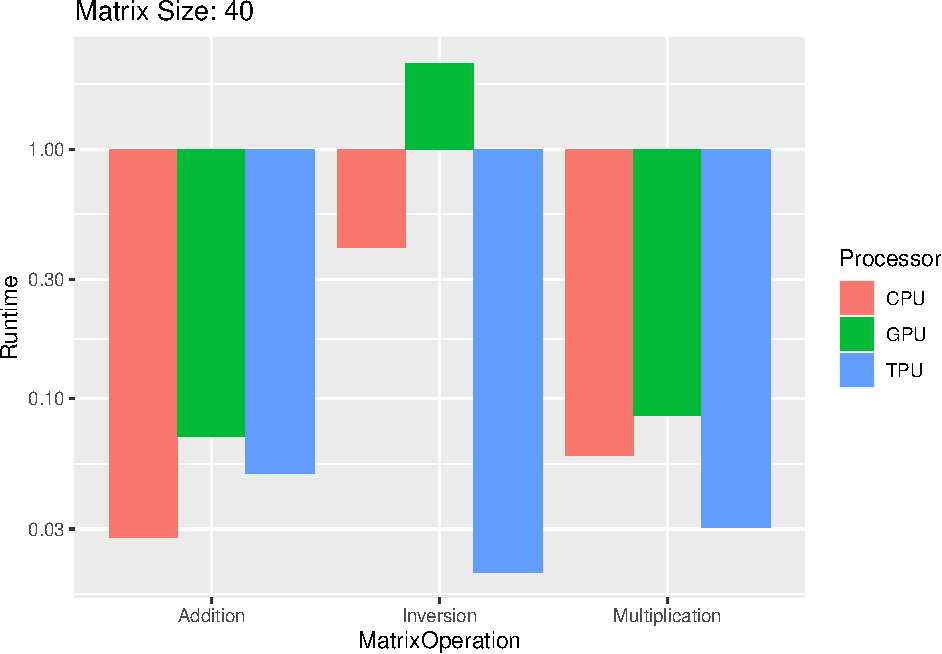
\includegraphics{main_files/figure-latex/unnamed-chunk-9-3.pdf}
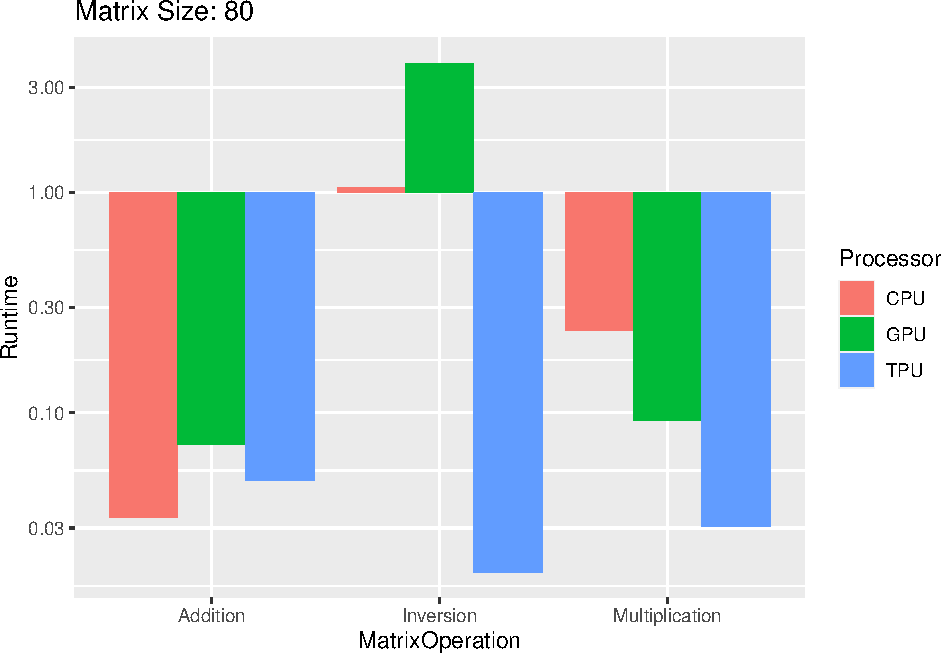
\includegraphics{main_files/figure-latex/unnamed-chunk-9-4.pdf}
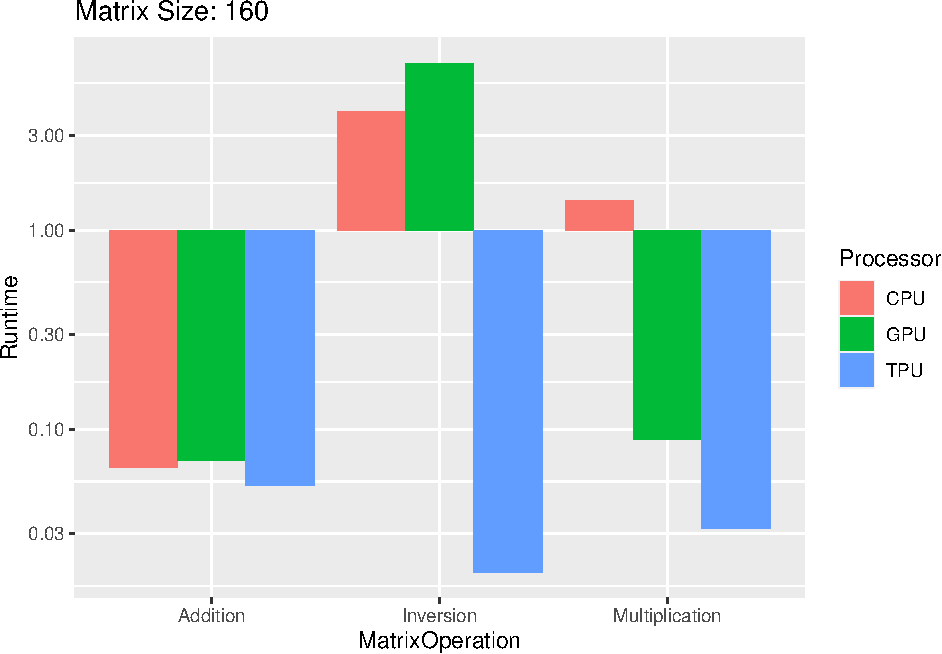
\includegraphics{main_files/figure-latex/unnamed-chunk-9-5.pdf}
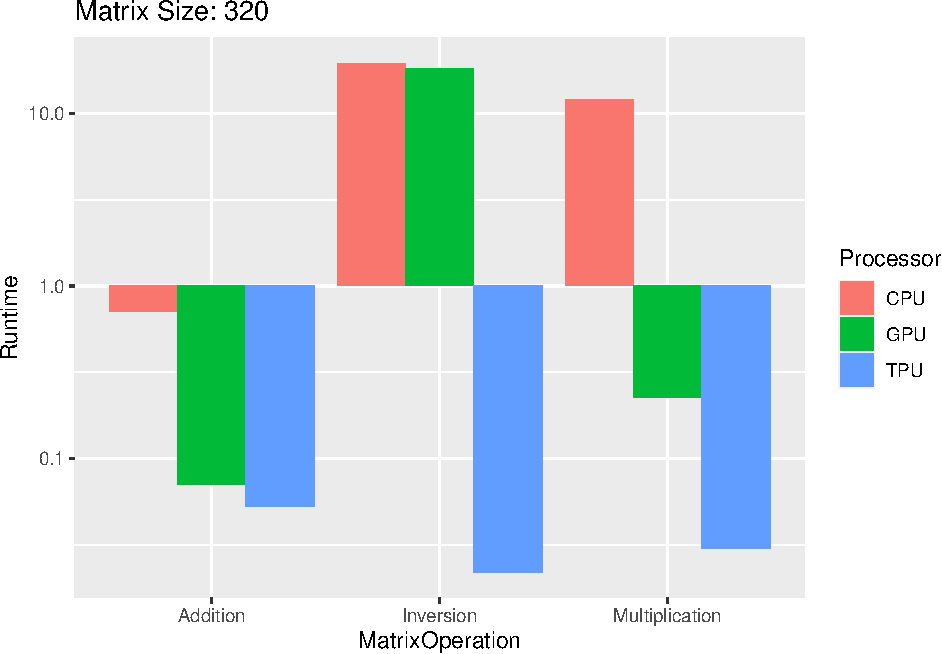
\includegraphics{main_files/figure-latex/unnamed-chunk-9-6.pdf}
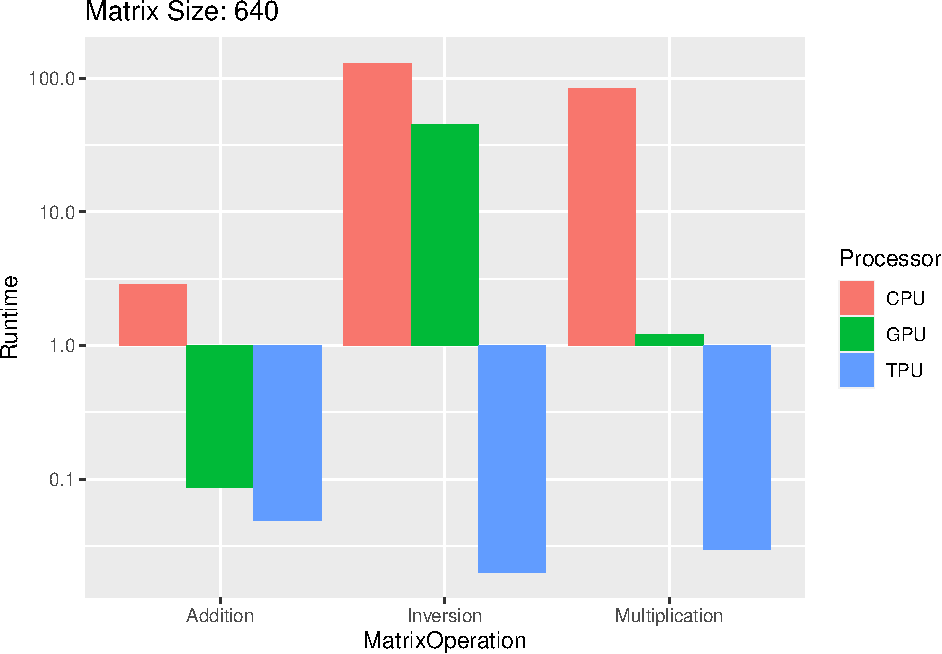
\includegraphics{main_files/figure-latex/unnamed-chunk-9-7.pdf}
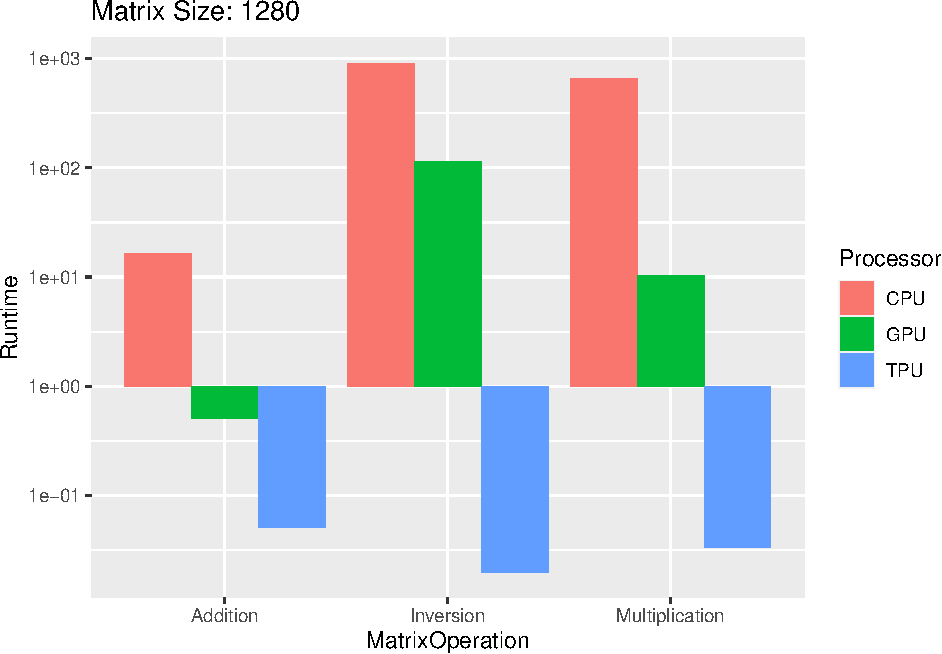
\includegraphics{main_files/figure-latex/unnamed-chunk-9-8.pdf}

\begin{Shaded}
\begin{Highlighting}[]
\ControlFlowTok{for}\NormalTok{(operation }\ControlFlowTok{in} \KeywordTok{unique}\NormalTok{(data}\OperatorTok{$}\NormalTok{MatrixOperation))\{}
\NormalTok{  p \textless{}{-}}\StringTok{ }\NormalTok{data }\OperatorTok{\%\textgreater{}\%}
\StringTok{    }\NormalTok{dplyr}\OperatorTok{::}\KeywordTok{filter}\NormalTok{(MatrixOperation }\OperatorTok{==}\StringTok{ }\NormalTok{operation) }\OperatorTok{\%\textgreater{}\%}
\StringTok{    }\KeywordTok{group\_by}\NormalTok{(MatrixSize, MatrixOperation, Processor) }\OperatorTok{\%\textgreater{}\%}
\StringTok{    }\KeywordTok{summarize}\NormalTok{(}\DataTypeTok{Runtime =} \KeywordTok{mean}\NormalTok{(Runtime)) }\OperatorTok{\%\textgreater{}\%}
\StringTok{    }\KeywordTok{ggplot}\NormalTok{(}\KeywordTok{aes}\NormalTok{(}\DataTypeTok{x =} \KeywordTok{as.factor}\NormalTok{(MatrixSize), }\DataTypeTok{y =}\NormalTok{ Runtime)) }\OperatorTok{+}
\StringTok{    }\CommentTok{\#geom\_boxplot(aes(fill = as.factor(Processor))) +}
\StringTok{    }\KeywordTok{geom\_bar}\NormalTok{(}\KeywordTok{aes}\NormalTok{(}\DataTypeTok{fill =} \KeywordTok{as.factor}\NormalTok{(Processor)), }\DataTypeTok{stat =} \StringTok{"identity"}\NormalTok{, }
             \DataTypeTok{alpha =} \DecValTok{1}\NormalTok{, }\DataTypeTok{position =} \StringTok{"dodge"}\NormalTok{) }\OperatorTok{+}
\StringTok{    }\KeywordTok{scale\_y\_log10}\NormalTok{() }\OperatorTok{+}
\StringTok{    }\KeywordTok{ggtitle}\NormalTok{(}\KeywordTok{paste0}\NormalTok{(}\StringTok{"Matrix Operation: "}\NormalTok{, operation)) }\OperatorTok{+}
\StringTok{    }\CommentTok{\#facet\_wrap( \textasciitilde{} MatrixOperation, scales = "free", nrow = 1) +}
\StringTok{    }\KeywordTok{guides}\NormalTok{(}\DataTypeTok{fill=}\KeywordTok{guide\_legend}\NormalTok{(}\DataTypeTok{title =} \StringTok{"Processor"}\NormalTok{))}
  \KeywordTok{print}\NormalTok{(p)}
\NormalTok{\}}
\end{Highlighting}
\end{Shaded}

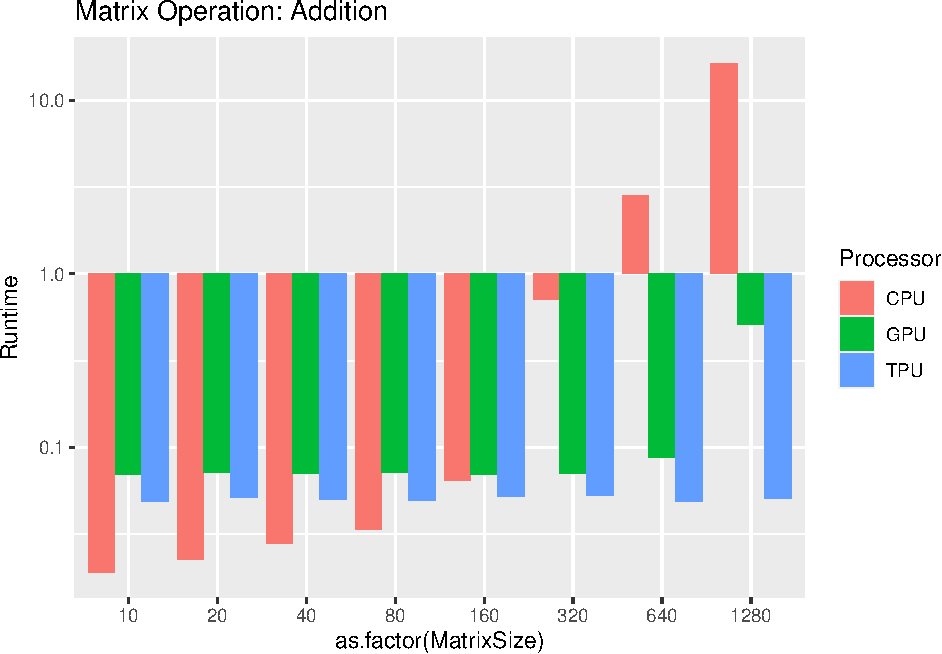
\includegraphics{main_files/figure-latex/unnamed-chunk-10-1.pdf}
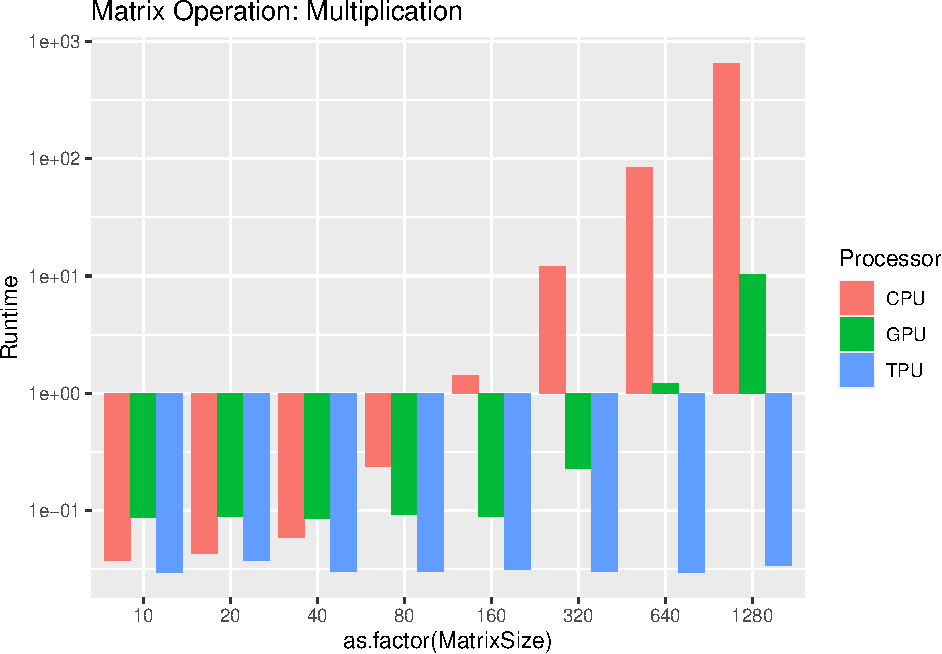
\includegraphics{main_files/figure-latex/unnamed-chunk-10-2.pdf}
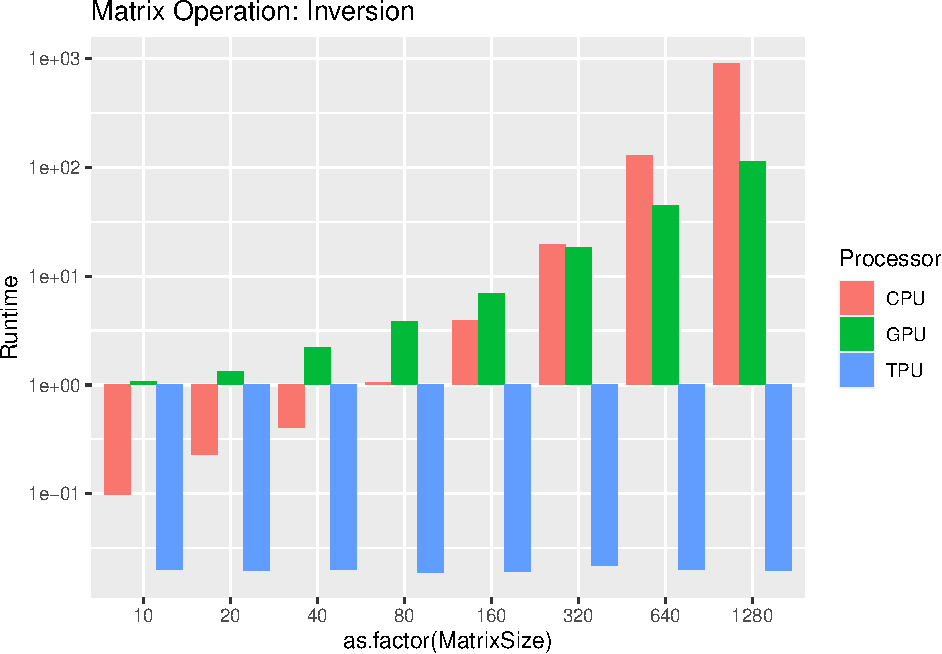
\includegraphics{main_files/figure-latex/unnamed-chunk-10-3.pdf}

\hypertarget{pros-cons-of-each-processor}{%
\subsection{Pros \& Cons of Each
Processor}\label{pros-cons-of-each-processor}}

CPU:

\begin{Shaded}
\begin{Highlighting}[]
\NormalTok{df\_cpu \textless{}{-}}\StringTok{ }\NormalTok{data[data}\OperatorTok{$}\NormalTok{Processor }\OperatorTok{==}\StringTok{ "CPU"}\NormalTok{,]}
\NormalTok{linreg\_cpu \textless{}{-}}\StringTok{ }\KeywordTok{lm}\NormalTok{(Runtime }\OperatorTok{\textasciitilde{}}\StringTok{ }\NormalTok{MatrixSize }\OperatorTok{+}\StringTok{ }\KeywordTok{as.factor}\NormalTok{(MatrixOperation), }
                 \DataTypeTok{data =}\NormalTok{ df\_cpu)}
\KeywordTok{summary}\NormalTok{(linreg\_cpu) }\OperatorTok{\%\textgreater{}\%}\StringTok{ }\KeywordTok{print}\NormalTok{()}
\end{Highlighting}
\end{Shaded}

\begin{verbatim}
## 
## Call:
## lm(formula = Runtime ~ MatrixSize + as.factor(MatrixOperation), 
##     data = df_cpu)
## 
## Residuals:
##     Min      1Q  Median      3Q     Max 
## -355.80  -71.41   -8.16   66.26  411.40 
## 
## Coefficients:
##                                            Estimate Std. Error t value Pr(>|t|)
## (Intercept)                              -120.02352   24.18254  -4.963 2.40e-06
## MatrixSize                                  0.38443    0.03081  12.477  < 2e-16
## as.factor(MatrixOperation)Inversion       130.34056   31.25182   4.171 5.89e-05
## as.factor(MatrixOperation)Multiplication   90.96003   31.25182   2.911  0.00433
##                                             
## (Intercept)                              ***
## MatrixSize                               ***
## as.factor(MatrixOperation)Inversion      ***
## as.factor(MatrixOperation)Multiplication ** 
## ---
## Signif. codes:  0 '***' 0.001 '**' 0.01 '*' 0.05 '.' 0.1 ' ' 1
## 
## Residual standard error: 139.8 on 116 degrees of freedom
## Multiple R-squared:    0.6,  Adjusted R-squared:  0.5896 
## F-statistic: 57.99 on 3 and 116 DF,  p-value: < 2.2e-16
\end{verbatim}

\begin{Shaded}
\begin{Highlighting}[]
\KeywordTok{plot}\NormalTok{(linreg\_cpu}\OperatorTok{$}\NormalTok{residuals)}
\KeywordTok{abline}\NormalTok{(}\DataTypeTok{h=}\DecValTok{0}\NormalTok{, }\DataTypeTok{col=}\StringTok{"red"}\NormalTok{)}
\end{Highlighting}
\end{Shaded}

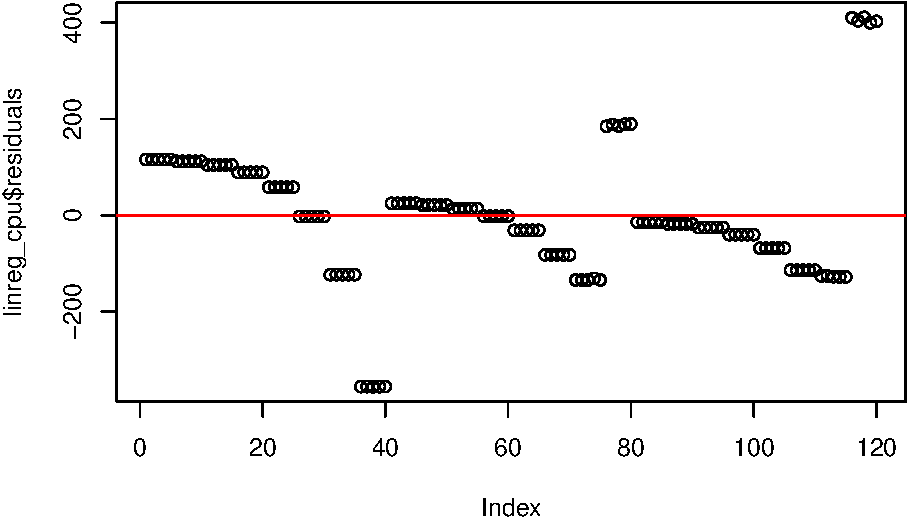
\includegraphics{main_files/figure-latex/unnamed-chunk-11-1.pdf}

\begin{Shaded}
\begin{Highlighting}[]
\KeywordTok{boxCox}\NormalTok{(linreg\_cpu)}
\end{Highlighting}
\end{Shaded}

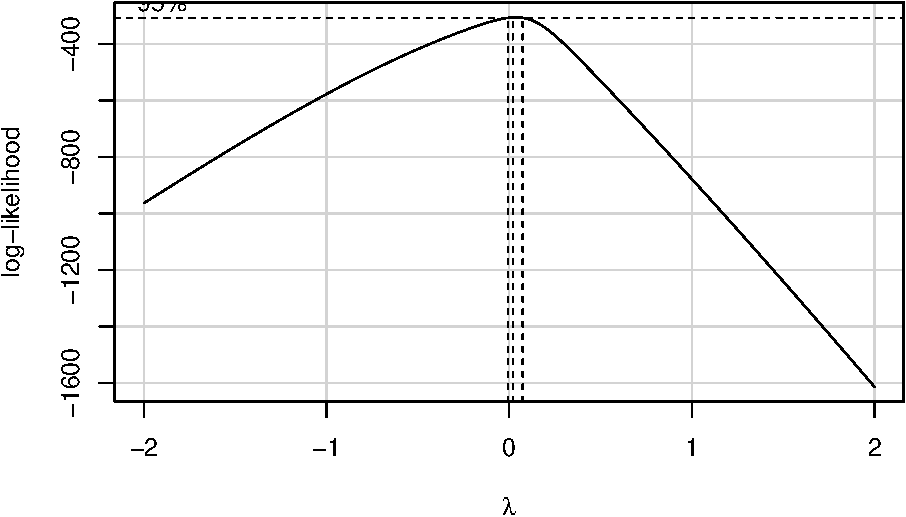
\includegraphics{main_files/figure-latex/unnamed-chunk-11-2.pdf}

\begin{Shaded}
\begin{Highlighting}[]
\NormalTok{linreg\_cpu\_trans \textless{}{-}}\StringTok{ }\KeywordTok{lm}\NormalTok{(}\KeywordTok{log}\NormalTok{(Runtime) }\OperatorTok{\textasciitilde{}}\StringTok{ }\NormalTok{MatrixSize }\OperatorTok{+}\StringTok{ }\KeywordTok{as.factor}\NormalTok{(MatrixOperation), }
                 \DataTypeTok{data =}\NormalTok{ df\_cpu)}
\KeywordTok{plot}\NormalTok{(linreg\_cpu\_trans}\OperatorTok{$}\NormalTok{fitted.values, linreg\_cpu\_trans}\OperatorTok{$}\NormalTok{residuals)}
\KeywordTok{abline}\NormalTok{(}\DataTypeTok{h=}\DecValTok{0}\NormalTok{, }\DataTypeTok{col=}\StringTok{"red"}\NormalTok{)}
\end{Highlighting}
\end{Shaded}

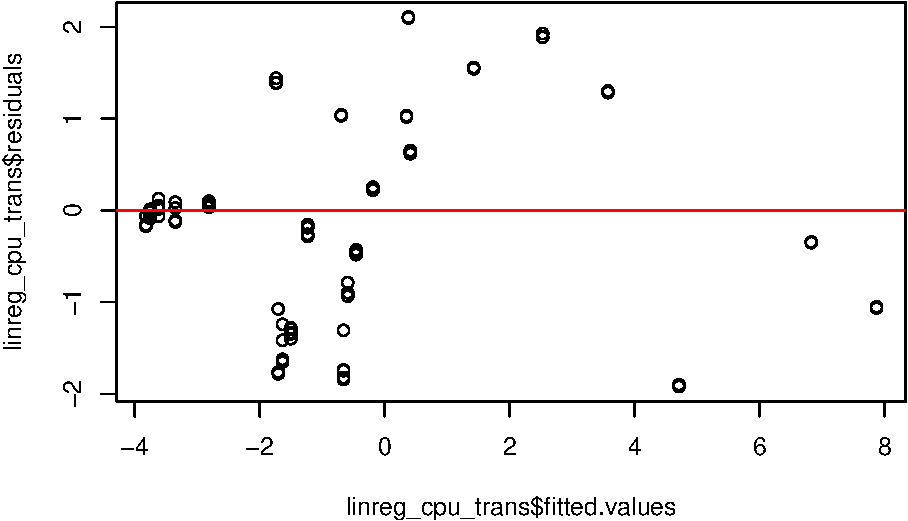
\includegraphics{main_files/figure-latex/unnamed-chunk-11-3.pdf} GPU:

\begin{Shaded}
\begin{Highlighting}[]
\NormalTok{df\_gpu \textless{}{-}}\StringTok{ }\NormalTok{data[(data}\OperatorTok{$}\NormalTok{Processor }\OperatorTok{==}\StringTok{ "GPU"}\NormalTok{) }\OperatorTok{\&}\StringTok{ }\NormalTok{(data}\OperatorTok{$}\NormalTok{MatrixOperation }\OperatorTok{!=}\StringTok{ "Multiplication"}\NormalTok{),]}
\NormalTok{linreg\_gpu \textless{}{-}}\StringTok{ }\KeywordTok{lm}\NormalTok{(Runtime }\OperatorTok{\textasciitilde{}}\StringTok{ }\NormalTok{MatrixSize }\OperatorTok{+}\StringTok{ }\KeywordTok{as.factor}\NormalTok{(MatrixOperation), }
                 \DataTypeTok{data =}\NormalTok{ df\_gpu)}
\KeywordTok{summary}\NormalTok{(linreg\_gpu) }\OperatorTok{\%\textgreater{}\%}\StringTok{ }\KeywordTok{print}\NormalTok{()}
\end{Highlighting}
\end{Shaded}

\begin{verbatim}
## 
## Call:
## lm(formula = Runtime ~ MatrixSize + as.factor(MatrixOperation), 
##     data = df_gpu)
## 
## Residuals:
##     Min      1Q  Median      3Q     Max 
## -41.981  -9.566  -2.974  10.907  47.604 
## 
## Coefficients:
##                                       Estimate Std. Error t value Pr(>|t|)    
## (Intercept)                         -13.920265   3.377960  -4.121 9.43e-05 ***
## MatrixSize                            0.044073   0.005066   8.699 4.57e-13 ***
## as.factor(MatrixOperation)Inversion  23.893954   4.195848   5.695 2.15e-07 ***
## ---
## Signif. codes:  0 '***' 0.001 '**' 0.01 '*' 0.05 '.' 0.1 ' ' 1
## 
## Residual standard error: 18.76 on 77 degrees of freedom
## Multiple R-squared:  0.584,  Adjusted R-squared:  0.5732 
## F-statistic: 54.05 on 2 and 77 DF,  p-value: 2.161e-15
\end{verbatim}

\begin{Shaded}
\begin{Highlighting}[]
\KeywordTok{plot}\NormalTok{(linreg\_gpu}\OperatorTok{$}\NormalTok{residuals)}
\KeywordTok{abline}\NormalTok{(}\DataTypeTok{h=}\DecValTok{0}\NormalTok{, }\DataTypeTok{col=}\StringTok{"red"}\NormalTok{)}
\end{Highlighting}
\end{Shaded}

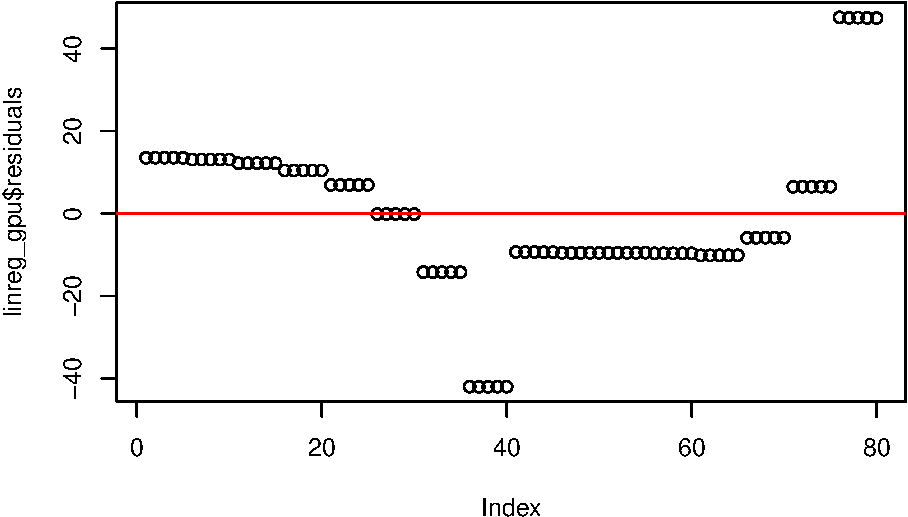
\includegraphics{main_files/figure-latex/unnamed-chunk-12-1.pdf}

\begin{Shaded}
\begin{Highlighting}[]
\KeywordTok{boxCox}\NormalTok{(linreg\_gpu)}
\end{Highlighting}
\end{Shaded}

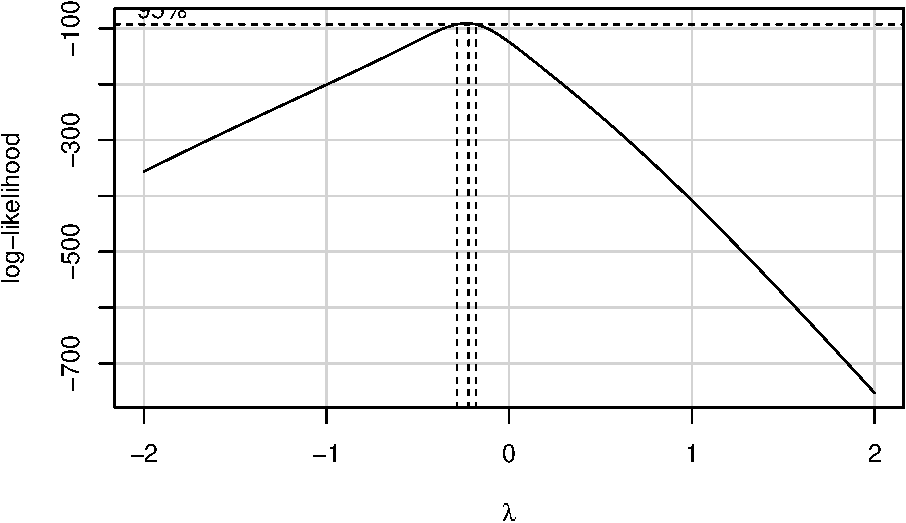
\includegraphics{main_files/figure-latex/unnamed-chunk-12-2.pdf}

\begin{Shaded}
\begin{Highlighting}[]
\NormalTok{linreg\_gpu\_trans \textless{}{-}}\StringTok{ }\KeywordTok{lm}\NormalTok{(}\KeywordTok{log10}\NormalTok{(Runtime) }\OperatorTok{\textasciitilde{}}\StringTok{ }\NormalTok{MatrixSize }\OperatorTok{+}
\StringTok{                         }\KeywordTok{as.factor}\NormalTok{(MatrixOperation), }\DataTypeTok{data =}\NormalTok{ df\_gpu)}
\KeywordTok{summary}\NormalTok{(linreg\_gpu\_trans)}
\end{Highlighting}
\end{Shaded}

\begin{verbatim}
## 
## Call:
## lm(formula = log10(Runtime) ~ MatrixSize + as.factor(MatrixOperation), 
##     data = df_gpu)
## 
## Residuals:
##      Min       1Q   Median       3Q      Max 
## -0.50239 -0.23761  0.09982  0.19255  0.44349 
## 
## Coefficients:
##                                       Estimate Std. Error t value Pr(>|t|)    
## (Intercept)                         -1.374e+00  5.133e-02  -26.77   <2e-16 ***
## MatrixSize                           1.075e-03  7.699e-05   13.96   <2e-16 ***
## as.factor(MatrixOperation)Inversion  1.894e+00  6.376e-02   29.70   <2e-16 ***
## ---
## Signif. codes:  0 '***' 0.001 '**' 0.01 '*' 0.05 '.' 0.1 ' ' 1
## 
## Residual standard error: 0.2851 on 77 degrees of freedom
## Multiple R-squared:  0.9333, Adjusted R-squared:  0.9315 
## F-statistic: 538.4 on 2 and 77 DF,  p-value: < 2.2e-16
\end{verbatim}

\begin{Shaded}
\begin{Highlighting}[]
\KeywordTok{plot}\NormalTok{(linreg\_gpu\_trans}\OperatorTok{$}\NormalTok{residuals)}
\KeywordTok{abline}\NormalTok{(}\DataTypeTok{h=}\DecValTok{0}\NormalTok{, }\DataTypeTok{col=}\StringTok{"red"}\NormalTok{)}
\end{Highlighting}
\end{Shaded}

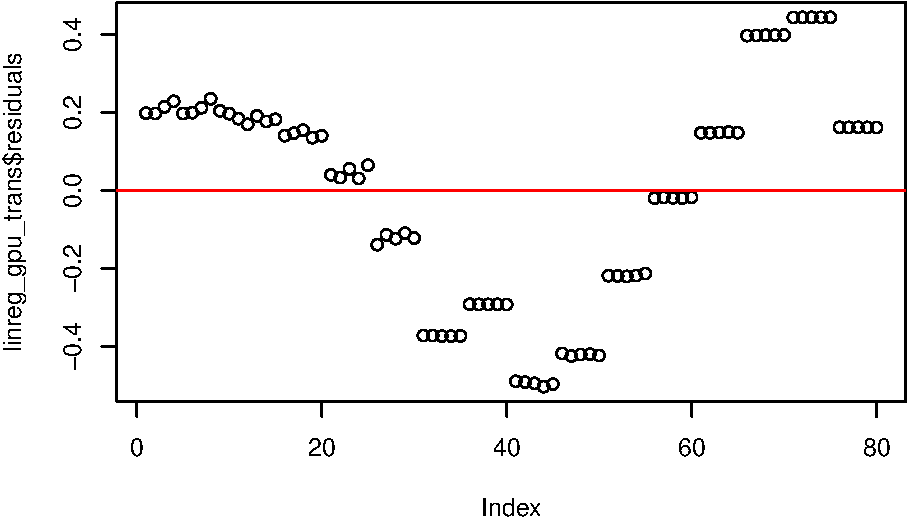
\includegraphics{main_files/figure-latex/unnamed-chunk-12-3.pdf}

TPU:

\begin{Shaded}
\begin{Highlighting}[]
\NormalTok{df\_tpu \textless{}{-}}\StringTok{ }\NormalTok{data[data}\OperatorTok{$}\NormalTok{Processor }\OperatorTok{==}\StringTok{ "TPU"}\NormalTok{,]}
\NormalTok{linreg\_tpu \textless{}{-}}\StringTok{ }\KeywordTok{lm}\NormalTok{(Runtime }\OperatorTok{\textasciitilde{}}\StringTok{ }\NormalTok{MatrixSize }\OperatorTok{+}\StringTok{ }\KeywordTok{as.factor}\NormalTok{(MatrixOperation), }
                 \DataTypeTok{data =}\NormalTok{ df\_tpu)}
\KeywordTok{summary}\NormalTok{(linreg\_tpu) }\OperatorTok{\%\textgreater{}\%}\StringTok{ }\KeywordTok{print}\NormalTok{()}
\end{Highlighting}
\end{Shaded}

\begin{verbatim}
## 
## Call:
## lm(formula = Runtime ~ MatrixSize + as.factor(MatrixOperation), 
##     data = df_tpu)
## 
## Residuals:
##        Min         1Q     Median         3Q        Max 
## -0.0034224 -0.0020056 -0.0010012 -0.0000435  0.0270875 
## 
## Coefficients:
##                                            Estimate Std. Error t value Pr(>|t|)
## (Intercept)                               5.039e-02  7.237e-04   69.62   <2e-16
## MatrixSize                                3.595e-07  9.221e-07    0.39    0.697
## as.factor(MatrixOperation)Inversion      -3.058e-02  9.353e-04  -32.70   <2e-16
## as.factor(MatrixOperation)Multiplication -1.877e-02  9.353e-04  -20.07   <2e-16
##                                             
## (Intercept)                              ***
## MatrixSize                                  
## as.factor(MatrixOperation)Inversion      ***
## as.factor(MatrixOperation)Multiplication ***
## ---
## Signif. codes:  0 '***' 0.001 '**' 0.01 '*' 0.05 '.' 0.1 ' ' 1
## 
## Residual standard error: 0.004183 on 116 degrees of freedom
## Multiple R-squared:  0.9036, Adjusted R-squared:  0.9012 
## F-statistic: 362.6 on 3 and 116 DF,  p-value: < 2.2e-16
\end{verbatim}

\begin{Shaded}
\begin{Highlighting}[]
\KeywordTok{plot}\NormalTok{(linreg\_tpu}\OperatorTok{$}\NormalTok{residuals)}
\KeywordTok{abline}\NormalTok{(}\DataTypeTok{h=}\DecValTok{0}\NormalTok{, }\DataTypeTok{col=}\StringTok{"red"}\NormalTok{)}
\end{Highlighting}
\end{Shaded}

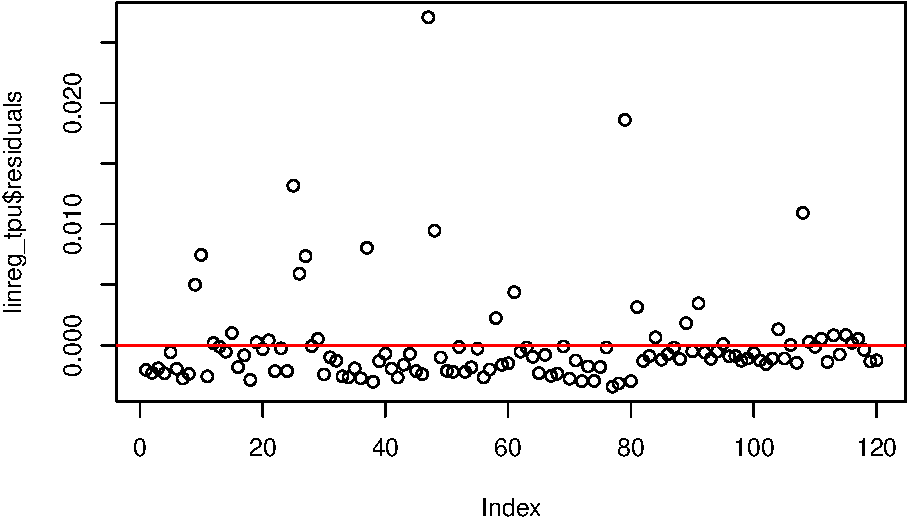
\includegraphics{main_files/figure-latex/unnamed-chunk-13-1.pdf}

\begin{Shaded}
\begin{Highlighting}[]
\KeywordTok{boxCox}\NormalTok{(linreg\_tpu)}
\end{Highlighting}
\end{Shaded}

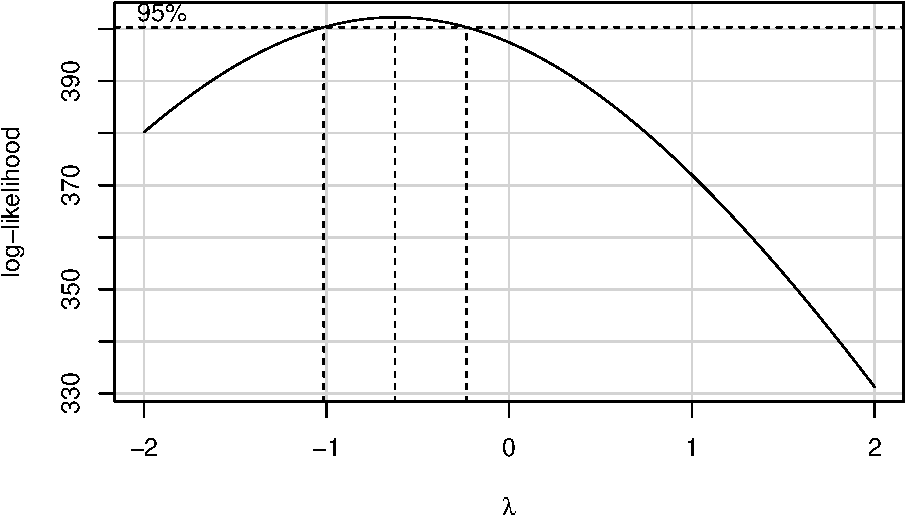
\includegraphics{main_files/figure-latex/unnamed-chunk-13-2.pdf}

\begin{Shaded}
\begin{Highlighting}[]
\NormalTok{linreg\_tpu\_trans \textless{}{-}}\StringTok{ }\KeywordTok{lm}\NormalTok{(}\KeywordTok{log10}\NormalTok{(Runtime) }\OperatorTok{\textasciitilde{}}\StringTok{ }\NormalTok{MatrixSize }\OperatorTok{+}
\StringTok{                         }\KeywordTok{as.factor}\NormalTok{(MatrixOperation), }\DataTypeTok{data =}\NormalTok{ df\_tpu)}
\KeywordTok{summary}\NormalTok{(linreg\_tpu\_trans) }\OperatorTok{\%\textgreater{}\%}\StringTok{ }\KeywordTok{print}\NormalTok{()}
\end{Highlighting}
\end{Shaded}

\begin{verbatim}
## 
## Call:
## lm(formula = log10(Runtime) ~ MatrixSize + as.factor(MatrixOperation), 
##     data = df_tpu)
## 
## Residuals:
##       Min        1Q    Median        3Q       Max 
## -0.043314 -0.023467 -0.014163  0.003178  0.273842 
## 
## Coefficients:
##                                            Estimate Std. Error  t value
## (Intercept)                              -1.299e+00  8.067e-03 -161.041
## MatrixSize                                4.439e-06  1.028e-05    0.432
## as.factor(MatrixOperation)Inversion      -4.050e-01  1.043e-02  -38.852
## as.factor(MatrixOperation)Multiplication -2.061e-01  1.043e-02  -19.770
##                                          Pr(>|t|)    
## (Intercept)                                <2e-16 ***
## MatrixSize                                  0.667    
## as.factor(MatrixOperation)Inversion        <2e-16 ***
## as.factor(MatrixOperation)Multiplication   <2e-16 ***
## ---
## Signif. codes:  0 '***' 0.001 '**' 0.01 '*' 0.05 '.' 0.1 ' ' 1
## 
## Residual standard error: 0.04662 on 116 degrees of freedom
## Multiple R-squared:  0.9287, Adjusted R-squared:  0.9268 
## F-statistic: 503.3 on 3 and 116 DF,  p-value: < 2.2e-16
\end{verbatim}

\begin{Shaded}
\begin{Highlighting}[]
\NormalTok{m \textless{}{-}}\StringTok{ }\KeywordTok{max}\NormalTok{(}\KeywordTok{abs}\NormalTok{(linreg\_tpu\_trans}\OperatorTok{$}\NormalTok{residuals))}
\KeywordTok{plot}\NormalTok{(linreg\_tpu\_trans}\OperatorTok{$}\NormalTok{residuals, }\DataTypeTok{ylim=}\KeywordTok{c}\NormalTok{(}\OperatorTok{{-}}\NormalTok{m, m))}
\KeywordTok{abline}\NormalTok{(}\DataTypeTok{h=}\DecValTok{0}\NormalTok{, }\DataTypeTok{col=}\StringTok{"red"}\NormalTok{)}
\end{Highlighting}
\end{Shaded}

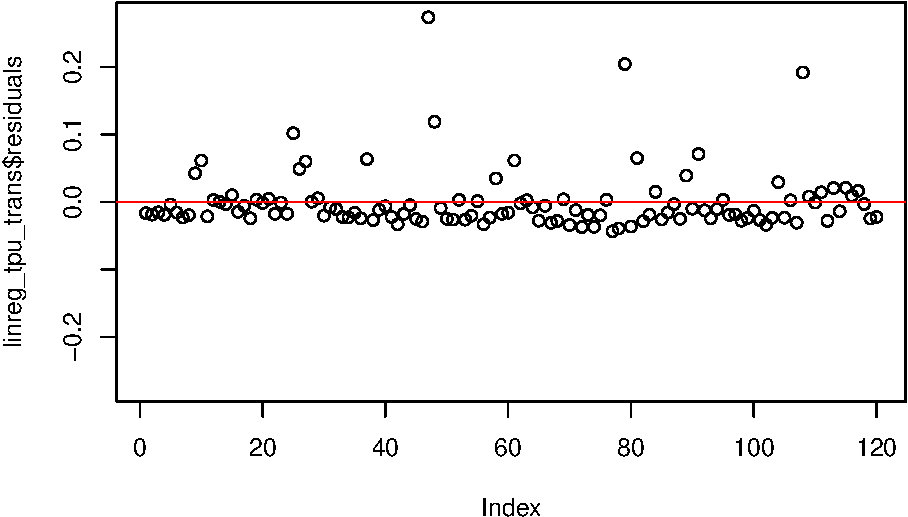
\includegraphics{main_files/figure-latex/unnamed-chunk-13-3.pdf}

GPU Addition

\begin{Shaded}
\begin{Highlighting}[]
\NormalTok{df\_small \textless{}{-}}\StringTok{ }\NormalTok{data[(data}\OperatorTok{$}\NormalTok{Processor }\OperatorTok{==}\StringTok{ "GPU"}\NormalTok{) }\OperatorTok{\&}\StringTok{ }\NormalTok{(data}\OperatorTok{$}\NormalTok{MatrixOperation }\OperatorTok{==}\StringTok{ "Addition"}\NormalTok{),]}
\NormalTok{linreg\_small \textless{}{-}}\StringTok{ }\KeywordTok{lm}\NormalTok{(Runtime }\OperatorTok{\textasciitilde{}}\StringTok{ }\NormalTok{MatrixSize, }\DataTypeTok{data =}\NormalTok{ df\_small)}
\KeywordTok{plot}\NormalTok{(linreg\_small}\OperatorTok{$}\NormalTok{residuals)}
\KeywordTok{abline}\NormalTok{(}\DataTypeTok{h=}\DecValTok{0}\NormalTok{, }\DataTypeTok{col=}\StringTok{"red"}\NormalTok{)}
\end{Highlighting}
\end{Shaded}

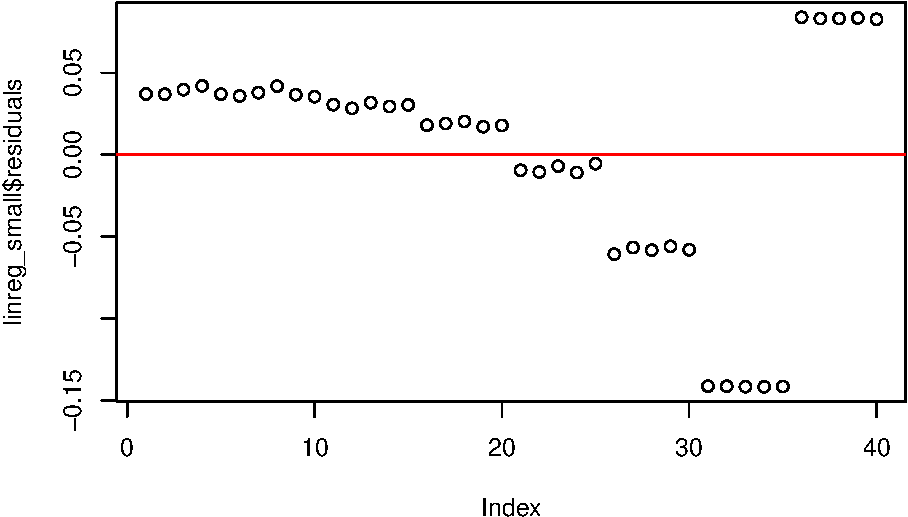
\includegraphics{main_files/figure-latex/unnamed-chunk-14-1.pdf}

\begin{Shaded}
\begin{Highlighting}[]
\KeywordTok{boxCox}\NormalTok{(linreg\_small, }\DataTypeTok{lambda =} \KeywordTok{seq}\NormalTok{(}\OperatorTok{{-}}\DecValTok{20}\NormalTok{, }\DecValTok{2}\NormalTok{, }\FloatTok{0.1}\NormalTok{))}
\end{Highlighting}
\end{Shaded}

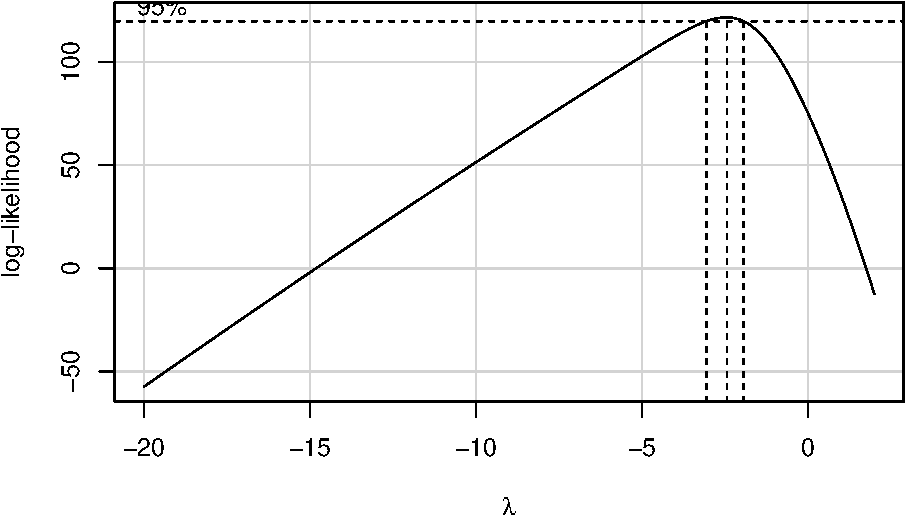
\includegraphics{main_files/figure-latex/unnamed-chunk-14-2.pdf}

\begin{Shaded}
\begin{Highlighting}[]
\NormalTok{linreg\_small\_transform \textless{}{-}}\StringTok{ }\KeywordTok{lm}\NormalTok{(}\KeywordTok{log10}\NormalTok{(Runtime) }\OperatorTok{\textasciitilde{}}\StringTok{ }\NormalTok{MatrixSize, }\DataTypeTok{data =}\NormalTok{ df\_small)}
\KeywordTok{plot}\NormalTok{(linreg\_small\_transform}\OperatorTok{$}\NormalTok{residuals)}
\KeywordTok{abline}\NormalTok{(}\DataTypeTok{h=}\DecValTok{0}\NormalTok{, }\DataTypeTok{col=}\StringTok{"red"}\NormalTok{)}
\end{Highlighting}
\end{Shaded}

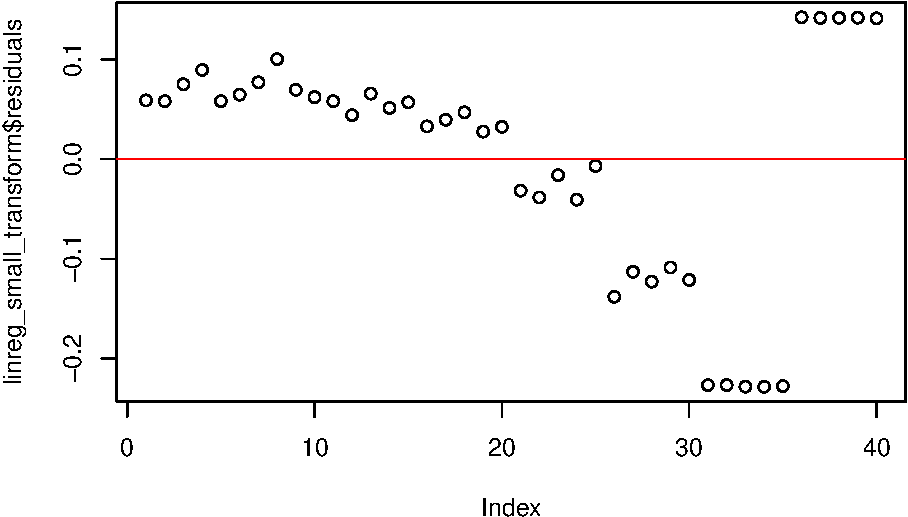
\includegraphics{main_files/figure-latex/unnamed-chunk-14-3.pdf}

\begin{Shaded}
\begin{Highlighting}[]
\KeywordTok{plot}\NormalTok{(df\_small}\OperatorTok{$}\NormalTok{MatrixSize, }\KeywordTok{log10}\NormalTok{(df\_small}\OperatorTok{$}\NormalTok{Runtime))}
\KeywordTok{abline}\NormalTok{(}\DataTypeTok{a=}\NormalTok{linreg\_small\_transform}\OperatorTok{$}\NormalTok{coefficients[}\DecValTok{1}\NormalTok{], }
       \DataTypeTok{b=}\NormalTok{linreg\_small\_transform}\OperatorTok{$}\NormalTok{coefficients[}\DecValTok{2}\NormalTok{])}
\end{Highlighting}
\end{Shaded}

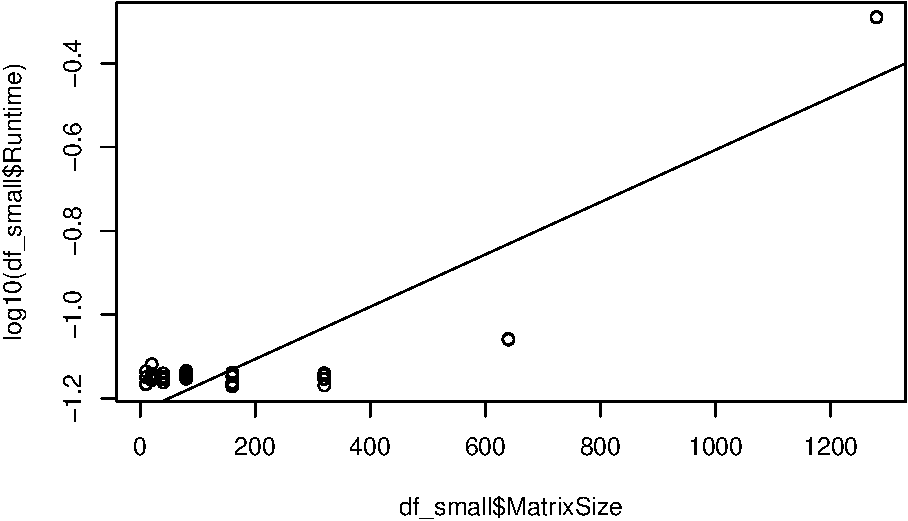
\includegraphics{main_files/figure-latex/unnamed-chunk-14-4.pdf}

GPU Multiplication

\begin{Shaded}
\begin{Highlighting}[]
\NormalTok{df\_small \textless{}{-}}\StringTok{ }\NormalTok{data[(data}\OperatorTok{$}\NormalTok{Processor }\OperatorTok{==}\StringTok{ "GPU"}\NormalTok{) }\OperatorTok{\&}\StringTok{ }\NormalTok{(data}\OperatorTok{$}\NormalTok{MatrixOperation }\OperatorTok{==}\StringTok{ "Multiplication"}\NormalTok{),]}
\NormalTok{linreg\_small \textless{}{-}}\StringTok{ }\KeywordTok{lm}\NormalTok{(Runtime }\OperatorTok{\textasciitilde{}}\StringTok{ }\NormalTok{MatrixSize, }\DataTypeTok{data =}\NormalTok{ df\_small)}
\KeywordTok{plot}\NormalTok{(linreg\_small}\OperatorTok{$}\NormalTok{residuals)}
\KeywordTok{abline}\NormalTok{(}\DataTypeTok{h=}\DecValTok{0}\NormalTok{, }\DataTypeTok{col=}\StringTok{"red"}\NormalTok{)}
\end{Highlighting}
\end{Shaded}

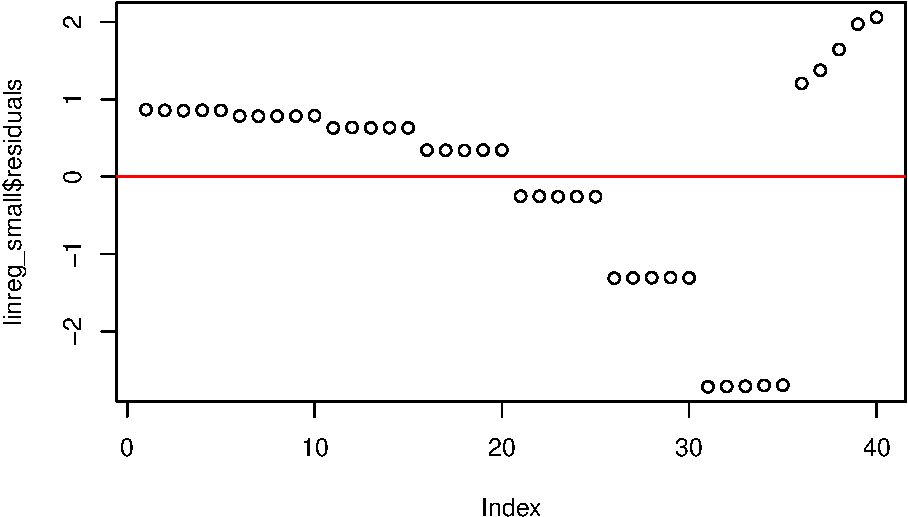
\includegraphics{main_files/figure-latex/unnamed-chunk-15-1.pdf}

\begin{Shaded}
\begin{Highlighting}[]
\KeywordTok{boxCox}\NormalTok{(linreg\_small, }\DataTypeTok{lambda =} \KeywordTok{seq}\NormalTok{(}\OperatorTok{{-}}\DecValTok{10}\NormalTok{, }\DecValTok{2}\NormalTok{, }\FloatTok{0.1}\NormalTok{))}
\end{Highlighting}
\end{Shaded}

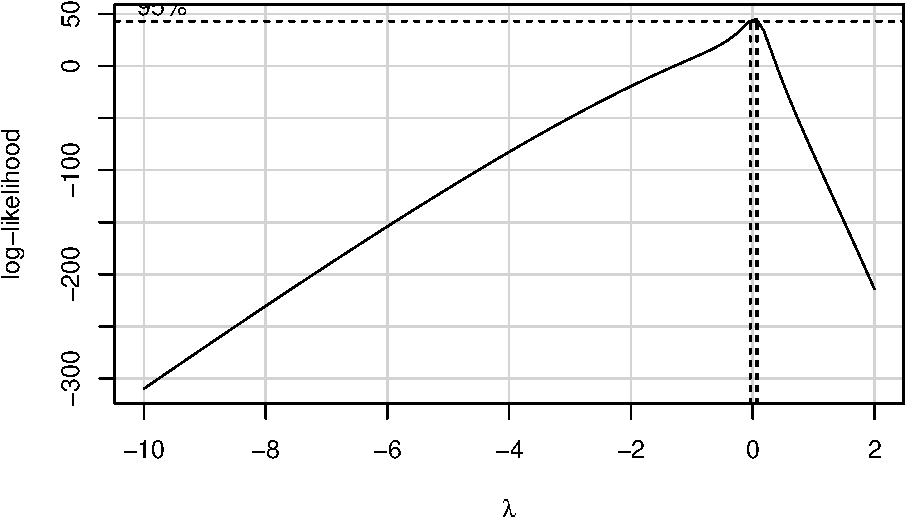
\includegraphics{main_files/figure-latex/unnamed-chunk-15-2.pdf}

\begin{Shaded}
\begin{Highlighting}[]
\NormalTok{linreg\_small\_transform \textless{}{-}}\StringTok{ }\KeywordTok{lm}\NormalTok{(}\KeywordTok{log10}\NormalTok{(Runtime) }\OperatorTok{\textasciitilde{}}\StringTok{ }\NormalTok{MatrixSize, }\DataTypeTok{data =}\NormalTok{ df\_small)}
\KeywordTok{summary}\NormalTok{(linreg\_small\_transform)}
\end{Highlighting}
\end{Shaded}

\begin{verbatim}
## 
## Call:
## lm(formula = log10(Runtime) ~ MatrixSize, data = df_small)
## 
## Residuals:
##       Min        1Q    Median        3Q       Max 
## -0.189553 -0.042371 -0.006256  0.062402  0.136090 
## 
## Coefficients:
##               Estimate Std. Error t value Pr(>|t|)    
## (Intercept) -1.148e+00  1.822e-02  -63.01   <2e-16 ***
## MatrixSize   1.715e-03  3.487e-05   49.19   <2e-16 ***
## ---
## Signif. codes:  0 '***' 0.001 '**' 0.01 '*' 0.05 '.' 0.1 ' ' 1
## 
## Residual standard error: 0.09131 on 38 degrees of freedom
## Multiple R-squared:  0.9845, Adjusted R-squared:  0.9841 
## F-statistic:  2419 on 1 and 38 DF,  p-value: < 2.2e-16
\end{verbatim}

\begin{Shaded}
\begin{Highlighting}[]
\KeywordTok{plot}\NormalTok{(linreg\_small\_transform}\OperatorTok{$}\NormalTok{residuals)}
\KeywordTok{abline}\NormalTok{(}\DataTypeTok{h=}\DecValTok{0}\NormalTok{, }\DataTypeTok{col=}\StringTok{"red"}\NormalTok{)}
\end{Highlighting}
\end{Shaded}

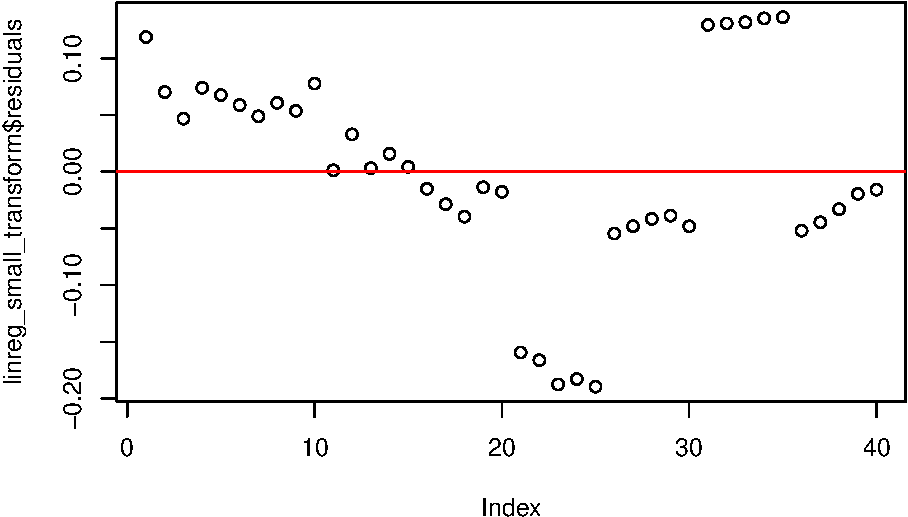
\includegraphics{main_files/figure-latex/unnamed-chunk-15-3.pdf}

\begin{Shaded}
\begin{Highlighting}[]
\KeywordTok{plot}\NormalTok{(df\_small}\OperatorTok{$}\NormalTok{MatrixSize, }\KeywordTok{log10}\NormalTok{(df\_small}\OperatorTok{$}\NormalTok{Runtime))}
\KeywordTok{abline}\NormalTok{(}\DataTypeTok{a=}\NormalTok{linreg\_small\_transform}\OperatorTok{$}\NormalTok{coefficients[}\DecValTok{1}\NormalTok{], }
       \DataTypeTok{b=}\NormalTok{linreg\_small\_transform}\OperatorTok{$}\NormalTok{coefficients[}\DecValTok{2}\NormalTok{])}
\end{Highlighting}
\end{Shaded}

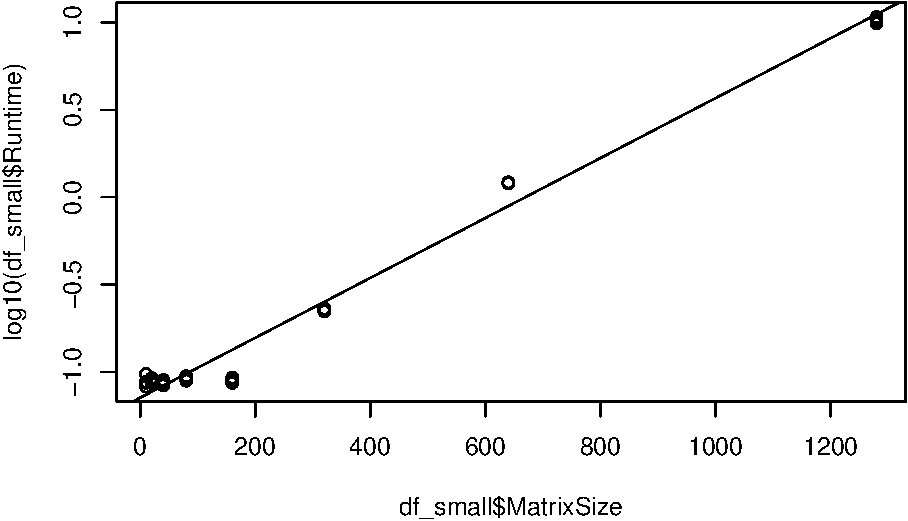
\includegraphics{main_files/figure-latex/unnamed-chunk-15-4.pdf}

GPU Inversion

\begin{Shaded}
\begin{Highlighting}[]
\NormalTok{df\_small \textless{}{-}}\StringTok{ }\NormalTok{data[(data}\OperatorTok{$}\NormalTok{Processor }\OperatorTok{==}\StringTok{ "GPU"}\NormalTok{) }\OperatorTok{\&}\StringTok{ }\NormalTok{(data}\OperatorTok{$}\NormalTok{MatrixOperation }\OperatorTok{==}\StringTok{ "Inversion"}\NormalTok{),]}
\NormalTok{linreg\_small \textless{}{-}}\StringTok{ }\KeywordTok{lm}\NormalTok{(Runtime }\OperatorTok{\textasciitilde{}}\StringTok{ }\NormalTok{MatrixSize, }\DataTypeTok{data =}\NormalTok{ df\_small)}
\KeywordTok{plot}\NormalTok{(linreg\_small}\OperatorTok{$}\NormalTok{fitted.values, linreg\_small}\OperatorTok{$}\NormalTok{residuals)}
\KeywordTok{abline}\NormalTok{(}\DataTypeTok{h=}\DecValTok{0}\NormalTok{, }\DataTypeTok{col=}\StringTok{"red"}\NormalTok{)}
\end{Highlighting}
\end{Shaded}

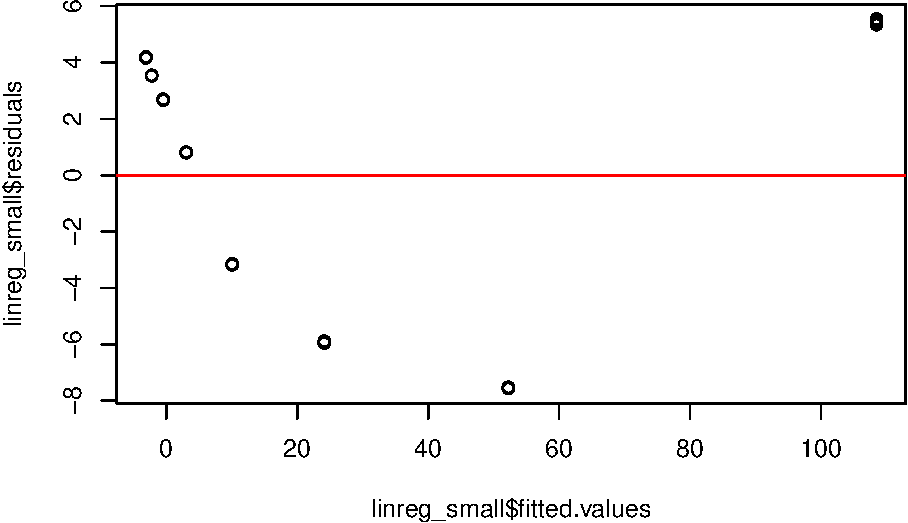
\includegraphics{main_files/figure-latex/unnamed-chunk-16-1.pdf}

\begin{Shaded}
\begin{Highlighting}[]
\KeywordTok{boxCox}\NormalTok{(linreg\_small, }\DataTypeTok{lambda =} \KeywordTok{seq}\NormalTok{(}\OperatorTok{{-}}\DecValTok{2}\NormalTok{, }\DecValTok{2}\NormalTok{, }\FloatTok{0.1}\NormalTok{))}
\end{Highlighting}
\end{Shaded}

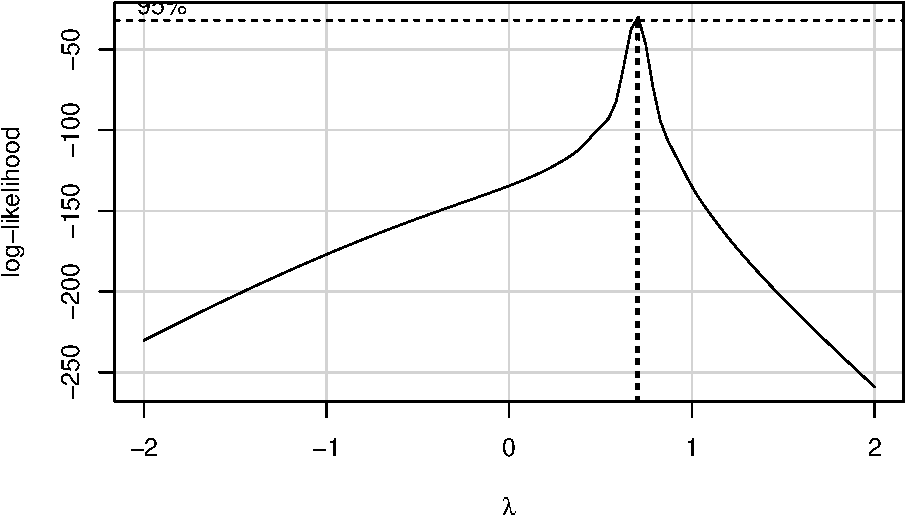
\includegraphics{main_files/figure-latex/unnamed-chunk-16-2.pdf}

\begin{Shaded}
\begin{Highlighting}[]
\NormalTok{linreg\_small\_transform \textless{}{-}}\StringTok{ }\KeywordTok{lm}\NormalTok{((Runtime}\OperatorTok{\^{}}\NormalTok{(}\DecValTok{2}\OperatorTok{/}\DecValTok{3}\NormalTok{)) }\OperatorTok{\textasciitilde{}}\StringTok{ }\NormalTok{MatrixSize, }\DataTypeTok{data =}\NormalTok{ df\_small)}
\KeywordTok{summary}\NormalTok{(linreg\_small\_transform)}
\end{Highlighting}
\end{Shaded}

\begin{verbatim}
## 
## Call:
## lm(formula = (Runtime^(2/3)) ~ MatrixSize, data = df_small)
## 
## Residuals:
##      Min       1Q   Median       3Q      Max 
## -0.19426 -0.14522 -0.04634  0.11432  0.27609 
## 
## Coefficients:
##              Estimate Std. Error t value Pr(>|t|)    
## (Intercept) 9.817e-01  3.581e-02   27.42   <2e-16 ***
## MatrixSize  1.773e-02  6.852e-05  258.71   <2e-16 ***
## ---
## Signif. codes:  0 '***' 0.001 '**' 0.01 '*' 0.05 '.' 0.1 ' ' 1
## 
## Residual standard error: 0.1794 on 38 degrees of freedom
## Multiple R-squared:  0.9994, Adjusted R-squared:  0.9994 
## F-statistic: 6.693e+04 on 1 and 38 DF,  p-value: < 2.2e-16
\end{verbatim}

\begin{Shaded}
\begin{Highlighting}[]
\CommentTok{\#plot(linreg\_small\_transform)}
\KeywordTok{plot}\NormalTok{(linreg\_small\_transform}\OperatorTok{$}\NormalTok{fitted.values, linreg\_small\_transform}\OperatorTok{$}\NormalTok{residuals)}
\KeywordTok{abline}\NormalTok{(}\DataTypeTok{h=}\DecValTok{0}\NormalTok{, }\DataTypeTok{col=}\StringTok{"red"}\NormalTok{)}
\end{Highlighting}
\end{Shaded}

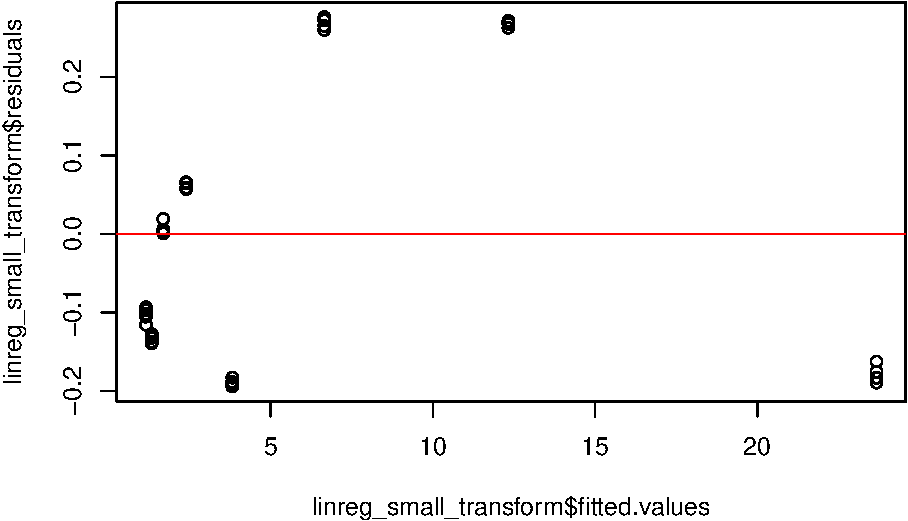
\includegraphics{main_files/figure-latex/unnamed-chunk-16-3.pdf}

\begin{Shaded}
\begin{Highlighting}[]
\KeywordTok{plot}\NormalTok{(df\_small}\OperatorTok{$}\NormalTok{MatrixSize, df\_small}\OperatorTok{$}\NormalTok{Runtime}\OperatorTok{\^{}}\NormalTok{(}\DecValTok{2}\OperatorTok{/}\DecValTok{3}\NormalTok{))}
\KeywordTok{abline}\NormalTok{(}\DataTypeTok{a=}\NormalTok{linreg\_small\_transform}\OperatorTok{$}\NormalTok{coefficients[}\DecValTok{1}\NormalTok{], }
       \DataTypeTok{b=}\NormalTok{linreg\_small\_transform}\OperatorTok{$}\NormalTok{coefficients[}\DecValTok{2}\NormalTok{])}
\end{Highlighting}
\end{Shaded}

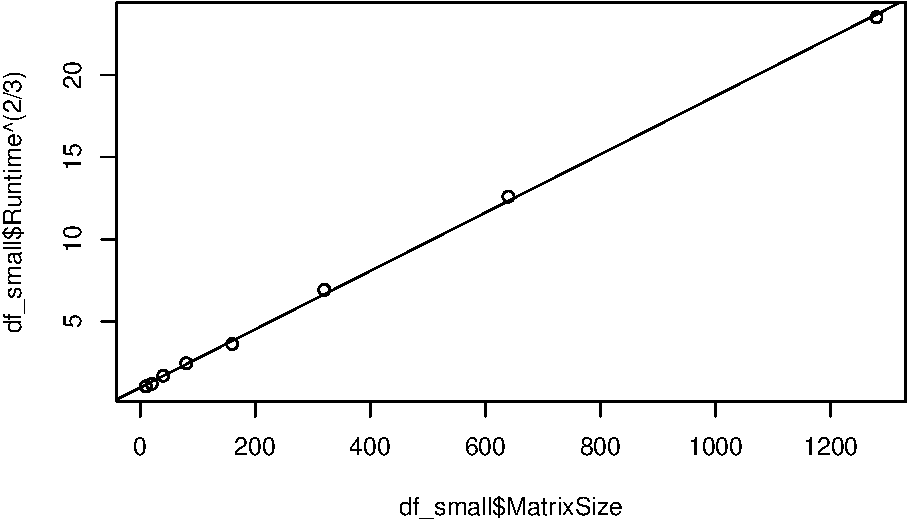
\includegraphics{main_files/figure-latex/unnamed-chunk-16-4.pdf}

TPU Addition

\begin{Shaded}
\begin{Highlighting}[]
\NormalTok{df\_small \textless{}{-}}\StringTok{ }\NormalTok{data[(data}\OperatorTok{$}\NormalTok{Processor }\OperatorTok{==}\StringTok{ "TPU"}\NormalTok{) }\OperatorTok{\&}\StringTok{ }\NormalTok{(data}\OperatorTok{$}\NormalTok{MatrixOperation }\OperatorTok{==}\StringTok{ "Addition"}\NormalTok{),]}
\NormalTok{linreg\_small \textless{}{-}}\StringTok{ }\KeywordTok{lm}\NormalTok{(Runtime }\OperatorTok{\textasciitilde{}}\StringTok{ }\NormalTok{MatrixSize, }\DataTypeTok{data =}\NormalTok{ df\_small)}
\KeywordTok{plot}\NormalTok{(linreg\_small}\OperatorTok{$}\NormalTok{residuals)}
\KeywordTok{abline}\NormalTok{(}\DataTypeTok{h=}\DecValTok{0}\NormalTok{, }\DataTypeTok{col=}\StringTok{"red"}\NormalTok{)}
\end{Highlighting}
\end{Shaded}

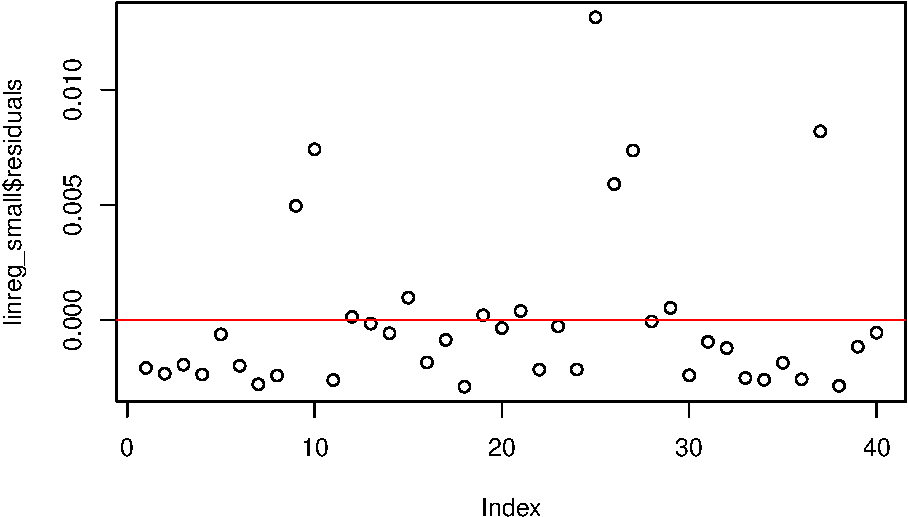
\includegraphics{main_files/figure-latex/unnamed-chunk-17-1.pdf}

\begin{Shaded}
\begin{Highlighting}[]
\KeywordTok{boxCox}\NormalTok{(linreg\_small, }\DataTypeTok{lambda =} \KeywordTok{seq}\NormalTok{(}\OperatorTok{{-}}\DecValTok{20}\NormalTok{, }\DecValTok{2}\NormalTok{, }\FloatTok{0.1}\NormalTok{))}
\end{Highlighting}
\end{Shaded}

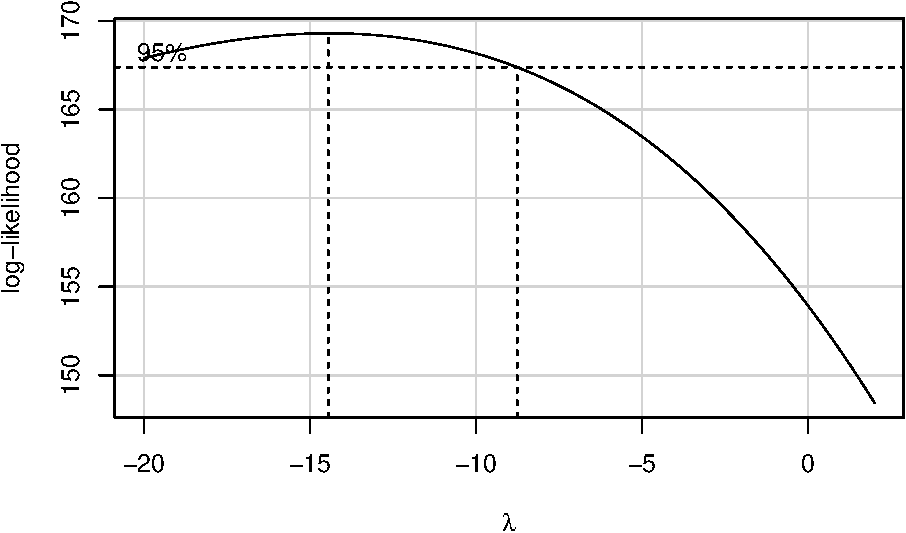
\includegraphics{main_files/figure-latex/unnamed-chunk-17-2.pdf}

\begin{Shaded}
\begin{Highlighting}[]
\NormalTok{linreg\_small\_transform \textless{}{-}}\StringTok{ }\KeywordTok{lm}\NormalTok{(}\KeywordTok{log10}\NormalTok{(Runtime) }\OperatorTok{\textasciitilde{}}\StringTok{ }\NormalTok{MatrixSize, }\DataTypeTok{data =}\NormalTok{ df\_small)}
\KeywordTok{summary}\NormalTok{(linreg\_small\_transform)}
\end{Highlighting}
\end{Shaded}

\begin{verbatim}
## 
## Call:
## lm(formula = log10(Runtime) ~ MatrixSize, data = df_small)
## 
## Residuals:
##       Min        1Q    Median        3Q       Max 
## -0.024742 -0.019679 -0.007998  0.002266  0.101552 
## 
## Coefficients:
##               Estimate Std. Error  t value Pr(>|t|)    
## (Intercept) -1.298e+00  5.948e-03 -218.276   <2e-16 ***
## MatrixSize   1.560e-06  1.138e-05    0.137    0.892    
## ---
## Signif. codes:  0 '***' 0.001 '**' 0.01 '*' 0.05 '.' 0.1 ' ' 1
## 
## Residual standard error: 0.02981 on 38 degrees of freedom
## Multiple R-squared:  0.0004943,  Adjusted R-squared:  -0.02581 
## F-statistic: 0.01879 on 1 and 38 DF,  p-value: 0.8917
\end{verbatim}

\begin{Shaded}
\begin{Highlighting}[]
\NormalTok{m \textless{}{-}}\StringTok{ }\KeywordTok{max}\NormalTok{(}\KeywordTok{abs}\NormalTok{(linreg\_small\_transform}\OperatorTok{$}\NormalTok{residuals))}
\KeywordTok{plot}\NormalTok{(linreg\_small\_transform}\OperatorTok{$}\NormalTok{residuals, }\DataTypeTok{ylim=}\KeywordTok{c}\NormalTok{(}\OperatorTok{{-}}\NormalTok{m, m))}
\KeywordTok{abline}\NormalTok{(}\DataTypeTok{h=}\DecValTok{0}\NormalTok{, }\DataTypeTok{col=}\StringTok{"red"}\NormalTok{)}
\end{Highlighting}
\end{Shaded}

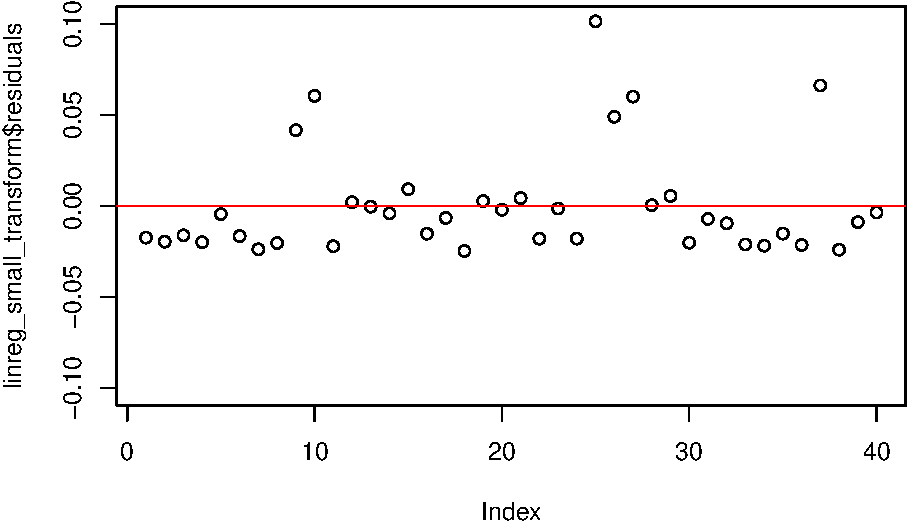
\includegraphics{main_files/figure-latex/unnamed-chunk-17-3.pdf}

TPU Multiplication

\begin{Shaded}
\begin{Highlighting}[]
\NormalTok{df\_small \textless{}{-}}\StringTok{ }\NormalTok{data[(data}\OperatorTok{$}\NormalTok{Processor }\OperatorTok{==}\StringTok{ "TPU"}\NormalTok{) }\OperatorTok{\&}\StringTok{ }\NormalTok{(data}\OperatorTok{$}\NormalTok{MatrixOperation }\OperatorTok{==}\StringTok{ "Multiplication"}\NormalTok{),]}
\NormalTok{linreg\_small \textless{}{-}}\StringTok{ }\KeywordTok{lm}\NormalTok{(Runtime }\OperatorTok{\textasciitilde{}}\StringTok{ }\NormalTok{MatrixSize, }\DataTypeTok{data =}\NormalTok{ df\_small)}
\KeywordTok{plot}\NormalTok{(linreg\_small}\OperatorTok{$}\NormalTok{residuals)}
\KeywordTok{abline}\NormalTok{(}\DataTypeTok{h=}\DecValTok{0}\NormalTok{, }\DataTypeTok{col=}\StringTok{"red"}\NormalTok{)}
\end{Highlighting}
\end{Shaded}

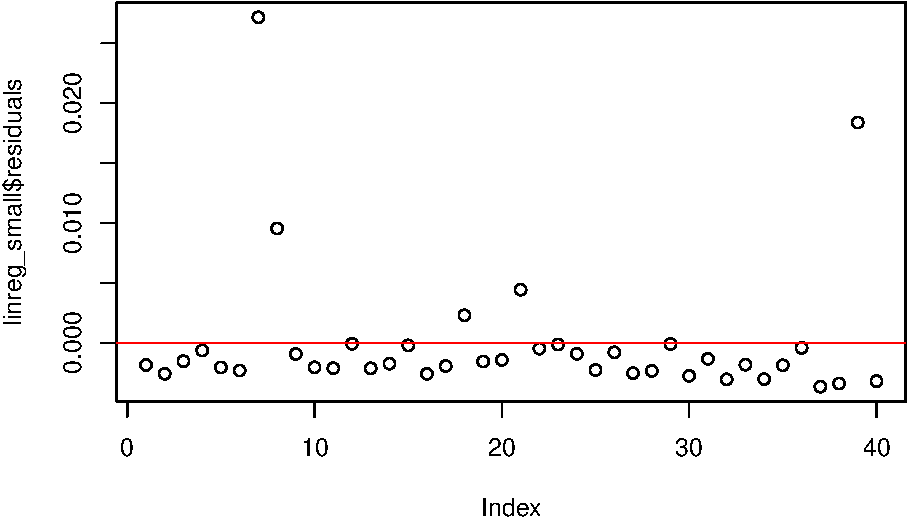
\includegraphics{main_files/figure-latex/unnamed-chunk-18-1.pdf}

\begin{Shaded}
\begin{Highlighting}[]
\KeywordTok{boxCox}\NormalTok{(linreg\_small, }\DataTypeTok{lambda =} \KeywordTok{seq}\NormalTok{(}\OperatorTok{{-}}\DecValTok{20}\NormalTok{, }\DecValTok{2}\NormalTok{, }\FloatTok{0.1}\NormalTok{))}
\end{Highlighting}
\end{Shaded}

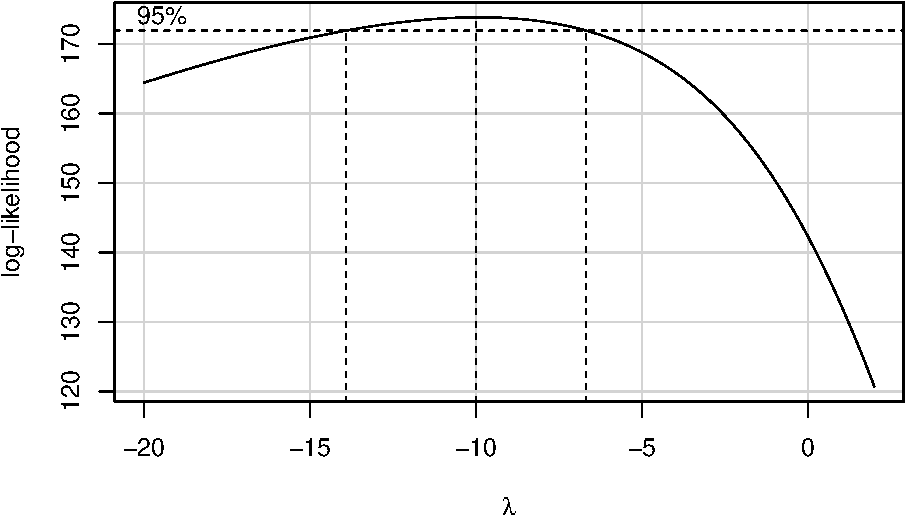
\includegraphics{main_files/figure-latex/unnamed-chunk-18-2.pdf}

\begin{Shaded}
\begin{Highlighting}[]
\NormalTok{linreg\_small\_transform \textless{}{-}}\StringTok{ }\KeywordTok{lm}\NormalTok{(}\KeywordTok{log10}\NormalTok{(Runtime) }\OperatorTok{\textasciitilde{}}\StringTok{ }\NormalTok{MatrixSize, }\DataTypeTok{data =}\NormalTok{ df\_small)}
\KeywordTok{summary}\NormalTok{(linreg\_small\_transform)}
\end{Highlighting}
\end{Shaded}

\begin{verbatim}
## 
## Call:
## lm(formula = log10(Runtime) ~ MatrixSize, data = df_small)
## 
## Residuals:
##       Min        1Q    Median        3Q       Max 
## -0.044167 -0.028197 -0.019721 -0.001056  0.274107 
## 
## Coefficients:
##               Estimate Std. Error  t value Pr(>|t|)    
## (Intercept) -1.506e+00  1.279e-02 -117.694   <2e-16 ***
## MatrixSize   5.326e-06  2.448e-05    0.218    0.829    
## ---
## Signif. codes:  0 '***' 0.001 '**' 0.01 '*' 0.05 '.' 0.1 ' ' 1
## 
## Residual standard error: 0.06411 on 38 degrees of freedom
## Multiple R-squared:  0.001244,   Adjusted R-squared:  -0.02504 
## F-statistic: 0.04734 on 1 and 38 DF,  p-value: 0.8289
\end{verbatim}

\begin{Shaded}
\begin{Highlighting}[]
\NormalTok{m \textless{}{-}}\StringTok{ }\KeywordTok{max}\NormalTok{(}\KeywordTok{abs}\NormalTok{(linreg\_small\_transform}\OperatorTok{$}\NormalTok{residuals))}
\KeywordTok{plot}\NormalTok{(linreg\_small\_transform}\OperatorTok{$}\NormalTok{residuals, }\DataTypeTok{ylim=}\KeywordTok{c}\NormalTok{(}\OperatorTok{{-}}\NormalTok{m, m))}
\KeywordTok{abline}\NormalTok{(}\DataTypeTok{h=}\DecValTok{0}\NormalTok{, }\DataTypeTok{col=}\StringTok{"red"}\NormalTok{)}
\end{Highlighting}
\end{Shaded}

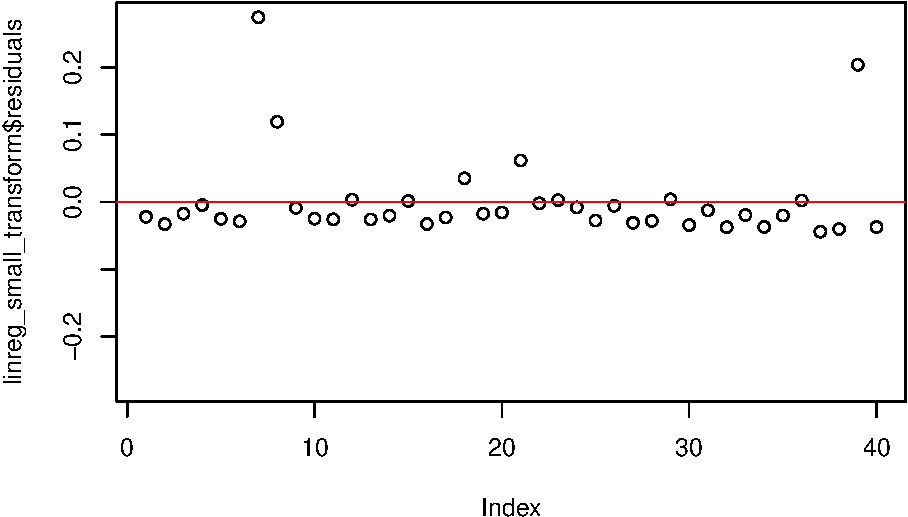
\includegraphics{main_files/figure-latex/unnamed-chunk-18-3.pdf}

TPU Inversion

\begin{Shaded}
\begin{Highlighting}[]
\NormalTok{df\_small \textless{}{-}}\StringTok{ }\NormalTok{data[(data}\OperatorTok{$}\NormalTok{Processor }\OperatorTok{==}\StringTok{ "TPU"}\NormalTok{) }\OperatorTok{\&}\StringTok{ }\NormalTok{(data}\OperatorTok{$}\NormalTok{MatrixOperation }\OperatorTok{==}\StringTok{ "Inversion"}\NormalTok{),]}
\NormalTok{linreg\_small \textless{}{-}}\StringTok{ }\KeywordTok{lm}\NormalTok{(Runtime }\OperatorTok{\textasciitilde{}}\StringTok{ }\NormalTok{MatrixSize, }\DataTypeTok{data =}\NormalTok{ df\_small)}
\KeywordTok{plot}\NormalTok{(linreg\_small}\OperatorTok{$}\NormalTok{residuals)}
\KeywordTok{abline}\NormalTok{(}\DataTypeTok{h=}\DecValTok{0}\NormalTok{, }\DataTypeTok{col=}\StringTok{"red"}\NormalTok{)}
\end{Highlighting}
\end{Shaded}

\includegraphics{main_files/figure-latex/unnamed-chunk-19-1.pdf}

\begin{Shaded}
\begin{Highlighting}[]
\KeywordTok{boxCox}\NormalTok{(linreg\_small, }\DataTypeTok{lambda =} \KeywordTok{seq}\NormalTok{(}\OperatorTok{{-}}\DecValTok{20}\NormalTok{, }\DecValTok{2}\NormalTok{, }\FloatTok{0.1}\NormalTok{))}
\end{Highlighting}
\end{Shaded}

\includegraphics{main_files/figure-latex/unnamed-chunk-19-2.pdf}

\begin{Shaded}
\begin{Highlighting}[]
\NormalTok{linreg\_small\_transform \textless{}{-}}\StringTok{ }\KeywordTok{lm}\NormalTok{(}\KeywordTok{log10}\NormalTok{(Runtime) }\OperatorTok{\textasciitilde{}}\StringTok{ }\NormalTok{MatrixSize, }\DataTypeTok{data =}\NormalTok{ df\_small)}
\KeywordTok{summary}\NormalTok{(linreg\_small\_transform)}
\end{Highlighting}
\end{Shaded}

\begin{verbatim}
## 
## Call:
## lm(formula = log10(Runtime) ~ MatrixSize, data = df_small)
## 
## Residuals:
##       Min        1Q    Median        3Q       Max 
## -0.033506 -0.023723 -0.012231  0.009422  0.192046 
## 
## Coefficients:
##               Estimate Std. Error  t value Pr(>|t|)    
## (Intercept) -1.705e+00  8.068e-03 -211.303   <2e-16 ***
## MatrixSize   6.430e-06  1.544e-05    0.416    0.679    
## ---
## Signif. codes:  0 '***' 0.001 '**' 0.01 '*' 0.05 '.' 0.1 ' ' 1
## 
## Residual standard error: 0.04043 on 38 degrees of freedom
## Multiple R-squared:  0.004544,   Adjusted R-squared:  -0.02165 
## F-statistic: 0.1734 on 1 and 38 DF,  p-value: 0.6794
\end{verbatim}

\begin{Shaded}
\begin{Highlighting}[]
\CommentTok{\#plot(linreg\_small\_transform)}
\NormalTok{m \textless{}{-}}\StringTok{ }\KeywordTok{max}\NormalTok{(}\KeywordTok{abs}\NormalTok{(linreg\_small\_transform}\OperatorTok{$}\NormalTok{residuals))}
\KeywordTok{plot}\NormalTok{(linreg\_small\_transform}\OperatorTok{$}\NormalTok{residuals, }\DataTypeTok{ylim=}\KeywordTok{c}\NormalTok{(}\OperatorTok{{-}}\NormalTok{m, m))}
\KeywordTok{abline}\NormalTok{(}\DataTypeTok{h=}\DecValTok{0}\NormalTok{, }\DataTypeTok{col=}\StringTok{"red"}\NormalTok{)}
\end{Highlighting}
\end{Shaded}

\includegraphics{main_files/figure-latex/unnamed-chunk-19-3.pdf}

ANOVA tests fixing matrix operation and matrix size

\begin{Shaded}
\begin{Highlighting}[]
\NormalTok{operation\_arr \textless{}{-}}\StringTok{ }\KeywordTok{unique}\NormalTok{(data}\OperatorTok{$}\NormalTok{MatrixOperation)}
\NormalTok{size\_arr \textless{}{-}}\StringTok{ }\KeywordTok{unique}\NormalTok{(data}\OperatorTok{$}\NormalTok{MatrixSize)}

\NormalTok{p\_val\_table \textless{}{-}}\StringTok{ }\KeywordTok{matrix}\NormalTok{(}\DecValTok{0}\NormalTok{, }\DataTypeTok{nrow =} \KeywordTok{length}\NormalTok{(size\_arr), }\DataTypeTok{ncol =} \DecValTok{2} \OperatorTok{*}\StringTok{ }\KeywordTok{length}\NormalTok{(operation\_arr))}
\KeywordTok{rownames}\NormalTok{(p\_val\_table) \textless{}{-}}\StringTok{ }\NormalTok{size\_arr}
\KeywordTok{colnames}\NormalTok{(p\_val\_table) \textless{}{-}}\StringTok{ }\KeywordTok{c}\NormalTok{(}\KeywordTok{paste0}\NormalTok{(}\StringTok{"GPU\_"}\NormalTok{, operation\_arr), }
                           \KeywordTok{paste0}\NormalTok{(}\StringTok{"TPU\_"}\NormalTok{, operation\_arr))}
\NormalTok{est\_table \textless{}{-}}\StringTok{ }\KeywordTok{matrix}\NormalTok{(}\DecValTok{0}\NormalTok{, }\DataTypeTok{nrow =} \KeywordTok{length}\NormalTok{(size\_arr), }\DataTypeTok{ncol =} \DecValTok{2} \OperatorTok{*}\StringTok{ }\KeywordTok{length}\NormalTok{(operation\_arr))}
\NormalTok{ci\_table \textless{}{-}}\StringTok{ }\KeywordTok{matrix}\NormalTok{(}\DecValTok{0}\NormalTok{, }\DataTypeTok{nrow =} \KeywordTok{length}\NormalTok{(size\_arr), }\DataTypeTok{ncol =} \DecValTok{2} \OperatorTok{*}\StringTok{ }\KeywordTok{length}\NormalTok{(operation\_arr))}

\ControlFlowTok{for}\NormalTok{(i }\ControlFlowTok{in} \DecValTok{1}\OperatorTok{:}\KeywordTok{length}\NormalTok{(operation\_arr))\{}
  \ControlFlowTok{for}\NormalTok{(j }\ControlFlowTok{in} \DecValTok{1}\OperatorTok{:}\KeywordTok{length}\NormalTok{(size\_arr))\{}
\NormalTok{    operation \textless{}{-}}\StringTok{ }\NormalTok{operation\_arr[i]}
\NormalTok{    size \textless{}{-}}\StringTok{ }\NormalTok{size\_arr[j]}
    
\NormalTok{    headline \textless{}{-}}\StringTok{ }\KeywordTok{paste0}\NormalTok{(}\StringTok{"Operation = "}\NormalTok{, operation, }\StringTok{"; Size = "}\NormalTok{, size)}
\NormalTok{    df\_small \textless{}{-}}\StringTok{ }\NormalTok{data[(data}\OperatorTok{$}\NormalTok{MatrixOperation }\OperatorTok{==}\StringTok{ }\NormalTok{operation) }\OperatorTok{\&}\StringTok{ }\NormalTok{(data}\OperatorTok{$}\NormalTok{MatrixSize }\OperatorTok{==}\StringTok{ }\NormalTok{size),]}
\NormalTok{    linreg\_small \textless{}{-}}\StringTok{ }\KeywordTok{lm}\NormalTok{(Runtime }\OperatorTok{\textasciitilde{}}\StringTok{ }\NormalTok{Processor, }\DataTypeTok{data =}\NormalTok{ df\_small)}
\NormalTok{    sm \textless{}{-}}\StringTok{ }\KeywordTok{summary}\NormalTok{(linreg\_small)}
    \KeywordTok{print}\NormalTok{(}\KeywordTok{paste0}\NormalTok{(headline, }\StringTok{": "}\NormalTok{, }\KeywordTok{round}\NormalTok{(sm}\OperatorTok{$}\NormalTok{adj.r.squared, }\DecValTok{3}\NormalTok{)))}
\NormalTok{    p\_val\_table[j, i] \textless{}{-}}\StringTok{ }\KeywordTok{as.numeric}\NormalTok{(sm}\OperatorTok{$}\NormalTok{coefficients[}\DecValTok{2}\NormalTok{,}\DecValTok{4}\NormalTok{])}
\NormalTok{    p\_val\_table[j, }\KeywordTok{length}\NormalTok{(operation\_arr)}\OperatorTok{+}\NormalTok{i] \textless{}{-}}\StringTok{ }\KeywordTok{as.numeric}\NormalTok{(sm}\OperatorTok{$}\NormalTok{coefficients[}\DecValTok{3}\NormalTok{,}\DecValTok{4}\NormalTok{])}
    
\NormalTok{    est\_table[j, i] \textless{}{-}}\StringTok{ }\KeywordTok{paste0}\NormalTok{(}\KeywordTok{round}\NormalTok{(sm}\OperatorTok{$}\NormalTok{coefficients[}\DecValTok{2}\NormalTok{,}\DecValTok{1}\NormalTok{], }\DecValTok{3}\NormalTok{), }\StringTok{" ("}\NormalTok{, }
                              \KeywordTok{round}\NormalTok{(sm}\OperatorTok{$}\NormalTok{coefficients[}\DecValTok{2}\NormalTok{,}\DecValTok{2}\NormalTok{], }\DecValTok{3}\NormalTok{), }\StringTok{")"}\NormalTok{)}
\NormalTok{    est\_table[j, }\KeywordTok{length}\NormalTok{(operation\_arr)}\OperatorTok{+}\NormalTok{i] \textless{}{-}}\StringTok{ }\KeywordTok{paste0}\NormalTok{(}\KeywordTok{round}\NormalTok{(sm}\OperatorTok{$}\NormalTok{coefficients[}\DecValTok{3}\NormalTok{,}\DecValTok{1}\NormalTok{], }\DecValTok{3}\NormalTok{),}
                                                    \StringTok{" ("}\NormalTok{, }
                                                    \KeywordTok{round}\NormalTok{(sm}\OperatorTok{$}\NormalTok{coefficients[}\DecValTok{3}\NormalTok{,}\DecValTok{2}\NormalTok{], }\DecValTok{3}\NormalTok{),}
                                                    \StringTok{")"}\NormalTok{)}
\NormalTok{    ci\_gpu \textless{}{-}}\StringTok{ }\KeywordTok{round}\NormalTok{(sm}\OperatorTok{$}\NormalTok{coefficients[}\DecValTok{2}\NormalTok{,}\DecValTok{1}\NormalTok{] }\OperatorTok{+}\StringTok{ }
\StringTok{                      }\KeywordTok{c}\NormalTok{(}\OperatorTok{{-}}\DecValTok{1}\NormalTok{,}\DecValTok{1}\NormalTok{)}\OperatorTok{*}\KeywordTok{qnorm}\NormalTok{(}\FloatTok{0.975}\NormalTok{)}\OperatorTok{*}\NormalTok{sm}\OperatorTok{$}\NormalTok{coefficients[}\DecValTok{2}\NormalTok{,}\DecValTok{2}\NormalTok{], }\DecValTok{3}\NormalTok{)}
\NormalTok{    ci\_tpu \textless{}{-}}\StringTok{ }\KeywordTok{round}\NormalTok{(sm}\OperatorTok{$}\NormalTok{coefficients[}\DecValTok{3}\NormalTok{,}\DecValTok{1}\NormalTok{] }\OperatorTok{+}\StringTok{ }
\StringTok{                      }\KeywordTok{c}\NormalTok{(}\OperatorTok{{-}}\DecValTok{1}\NormalTok{,}\DecValTok{1}\NormalTok{)}\OperatorTok{*}\KeywordTok{qnorm}\NormalTok{(}\FloatTok{0.975}\NormalTok{)}\OperatorTok{*}\NormalTok{sm}\OperatorTok{$}\NormalTok{coefficients[}\DecValTok{3}\NormalTok{,}\DecValTok{2}\NormalTok{], }\DecValTok{3}\NormalTok{)}
\NormalTok{    ci\_table[j, i] \textless{}{-}}\StringTok{ }\KeywordTok{paste0}\NormalTok{(}\StringTok{"("}\NormalTok{, ci\_gpu[}\DecValTok{1}\NormalTok{], }\StringTok{" to "}\NormalTok{, ci\_gpu[}\DecValTok{2}\NormalTok{], }\StringTok{")"}\NormalTok{)}
\NormalTok{    ci\_table[j, }\KeywordTok{length}\NormalTok{(operation\_arr)}\OperatorTok{+}\NormalTok{i] \textless{}{-}}\StringTok{ }\KeywordTok{paste0}\NormalTok{(}\StringTok{"("}\NormalTok{, ci\_tpu[}\DecValTok{1}\NormalTok{], }\StringTok{" to "}\NormalTok{,}
\NormalTok{                                                   ci\_tpu[}\DecValTok{2}\NormalTok{], }\StringTok{")"}\NormalTok{)}
    \CommentTok{\#print(headline)}
    \CommentTok{\#print(summary(linreg\_small))}
\NormalTok{    m \textless{}{-}}\StringTok{ }\KeywordTok{max}\NormalTok{(}\KeywordTok{abs}\NormalTok{(linreg\_small}\OperatorTok{$}\NormalTok{residuals))}
    \KeywordTok{plot}\NormalTok{(linreg\_small}\OperatorTok{$}\NormalTok{fitted.values, linreg\_small}\OperatorTok{$}\NormalTok{residuals, }\DataTypeTok{main =}\NormalTok{ headline,}
         \DataTypeTok{xlab =} \StringTok{"Fitted Values"}\NormalTok{, }\DataTypeTok{ylab =} \StringTok{"Residuals"}\NormalTok{, }\DataTypeTok{ylim=}\KeywordTok{c}\NormalTok{(}\OperatorTok{{-}}\NormalTok{m, m))}
    \KeywordTok{abline}\NormalTok{(}\DataTypeTok{h=}\DecValTok{0}\NormalTok{, }\DataTypeTok{col=}\StringTok{"red"}\NormalTok{)}
\NormalTok{  \}}
\NormalTok{\}}
\end{Highlighting}
\end{Shaded}

\begin{verbatim}
## [1] "Operation = Addition; Size = 10: 0.995"
\end{verbatim}

\includegraphics{main_files/figure-latex/unnamed-chunk-20-1.pdf}

\begin{verbatim}
## [1] "Operation = Addition; Size = 20: 0.977"
\end{verbatim}

\includegraphics{main_files/figure-latex/unnamed-chunk-20-2.pdf}

\begin{verbatim}
## [1] "Operation = Addition; Size = 40: 0.993"
\end{verbatim}

\includegraphics{main_files/figure-latex/unnamed-chunk-20-3.pdf}

\begin{verbatim}
## [1] "Operation = Addition; Size = 80: 0.982"
\end{verbatim}

\includegraphics{main_files/figure-latex/unnamed-chunk-20-4.pdf}

\begin{verbatim}
## [1] "Operation = Addition; Size = 160: 0.764"
\end{verbatim}

\includegraphics{main_files/figure-latex/unnamed-chunk-20-5.pdf}

\begin{verbatim}
## [1] "Operation = Addition; Size = 320: 0.999"
\end{verbatim}

\includegraphics{main_files/figure-latex/unnamed-chunk-20-6.pdf}

\begin{verbatim}
## [1] "Operation = Addition; Size = 640: 1"
\end{verbatim}

\includegraphics{main_files/figure-latex/unnamed-chunk-20-7.pdf}

\begin{verbatim}
## [1] "Operation = Addition; Size = 1280: 1"
\end{verbatim}

\includegraphics{main_files/figure-latex/unnamed-chunk-20-8.pdf}

\begin{verbatim}
## [1] "Operation = Multiplication; Size = 10: 0.904"
\end{verbatim}

\includegraphics{main_files/figure-latex/unnamed-chunk-20-9.pdf}

\begin{verbatim}
## [1] "Operation = Multiplication; Size = 20: 0.873"
\end{verbatim}

\includegraphics{main_files/figure-latex/unnamed-chunk-20-10.pdf}

\begin{verbatim}
## [1] "Operation = Multiplication; Size = 40: 0.991"
\end{verbatim}

\includegraphics{main_files/figure-latex/unnamed-chunk-20-11.pdf}

\begin{verbatim}
## [1] "Operation = Multiplication; Size = 80: 0.991"
\end{verbatim}

\includegraphics{main_files/figure-latex/unnamed-chunk-20-12.pdf}

\begin{verbatim}
## [1] "Operation = Multiplication; Size = 160: 1"
\end{verbatim}

\includegraphics{main_files/figure-latex/unnamed-chunk-20-13.pdf}

\begin{verbatim}
## [1] "Operation = Multiplication; Size = 320: 1"
\end{verbatim}

\includegraphics{main_files/figure-latex/unnamed-chunk-20-14.pdf}

\begin{verbatim}
## [1] "Operation = Multiplication; Size = 640: 1"
\end{verbatim}

\includegraphics{main_files/figure-latex/unnamed-chunk-20-15.pdf}

\begin{verbatim}
## [1] "Operation = Multiplication; Size = 1280: 1"
\end{verbatim}

\includegraphics{main_files/figure-latex/unnamed-chunk-20-16.pdf}

\begin{verbatim}
## [1] "Operation = Inversion; Size = 10: 0.999"
\end{verbatim}

\includegraphics{main_files/figure-latex/unnamed-chunk-20-17.pdf}

\begin{verbatim}
## [1] "Operation = Inversion; Size = 20: 1"
\end{verbatim}

\includegraphics{main_files/figure-latex/unnamed-chunk-20-18.pdf}

\begin{verbatim}
## [1] "Operation = Inversion; Size = 40: 1"
\end{verbatim}

\includegraphics{main_files/figure-latex/unnamed-chunk-20-19.pdf}

\begin{verbatim}
## [1] "Operation = Inversion; Size = 80: 1"
\end{verbatim}

\includegraphics{main_files/figure-latex/unnamed-chunk-20-20.pdf}

\begin{verbatim}
## [1] "Operation = Inversion; Size = 160: 1"
\end{verbatim}

\includegraphics{main_files/figure-latex/unnamed-chunk-20-21.pdf}

\begin{verbatim}
## [1] "Operation = Inversion; Size = 320: 1"
\end{verbatim}

\includegraphics{main_files/figure-latex/unnamed-chunk-20-22.pdf}

\begin{verbatim}
## [1] "Operation = Inversion; Size = 640: 1"
\end{verbatim}

\includegraphics{main_files/figure-latex/unnamed-chunk-20-23.pdf}

\begin{verbatim}
## [1] "Operation = Inversion; Size = 1280: 1"
\end{verbatim}

\includegraphics{main_files/figure-latex/unnamed-chunk-20-24.pdf}

\begin{Shaded}
\begin{Highlighting}[]
\CommentTok{\#print(p\_val\_table)}

\NormalTok{parse\_number \textless{}{-}}\StringTok{ }\ControlFlowTok{function}\NormalTok{(x)\{}
\NormalTok{  ret \textless{}{-}}\StringTok{ }\KeywordTok{paste0}\NormalTok{(}\StringTok{"$"}\NormalTok{, }\KeywordTok{str\_replace\_all}\NormalTok{(}\KeywordTok{formatC}\NormalTok{(x, }\DataTypeTok{digits=}\DecValTok{4}\NormalTok{), }\StringTok{"e"}\NormalTok{, }\StringTok{" }\CharTok{\textbackslash{}t}\StringTok{imes 10\^{}\{"}\NormalTok{))}
  \ControlFlowTok{if}\NormalTok{(}\KeywordTok{str\_detect}\NormalTok{(ret, }\StringTok{"}\CharTok{\textbackslash{}t}\StringTok{imes"}\NormalTok{))\{}
\NormalTok{    ret \textless{}{-}}\StringTok{ }\KeywordTok{paste0}\NormalTok{(ret, }\StringTok{"\}"}\NormalTok{)}
\NormalTok{  \}}
\NormalTok{  ret \textless{}{-}}\StringTok{ }\KeywordTok{paste0}\NormalTok{(ret, }\StringTok{"$"}\NormalTok{)}
\NormalTok{  ret}
\NormalTok{\}}
\NormalTok{p\_val\_display \textless{}{-}}\StringTok{ }\NormalTok{p\_val\_table}
\ControlFlowTok{for}\NormalTok{(i }\ControlFlowTok{in} \DecValTok{1}\OperatorTok{:}\KeywordTok{nrow}\NormalTok{(p\_val\_display))\{}
  \ControlFlowTok{for}\NormalTok{(j }\ControlFlowTok{in} \DecValTok{1}\OperatorTok{:}\KeywordTok{ncol}\NormalTok{(p\_val\_display))\{}
\NormalTok{    p\_val\_display[i, j] \textless{}{-}}\StringTok{ }\KeywordTok{parse\_number}\NormalTok{(p\_val\_table[i, j])}
\NormalTok{  \}}
\NormalTok{\}}
\CommentTok{\#p\_val\_display \%\textgreater{}\% print()}

\ControlFlowTok{for}\NormalTok{(i }\ControlFlowTok{in} \DecValTok{1}\OperatorTok{:}\KeywordTok{nrow}\NormalTok{(p\_val\_display))\{}
  \CommentTok{\#paste0(p\_val\_display[i,], collapse = " \& ") \%\textgreater{}\% print()}
  \CommentTok{\#paste0(ci\_table[i,], collapse = " \& ") \%\textgreater{}\% print()}
\NormalTok{\}}
\end{Highlighting}
\end{Shaded}

\begin{Shaded}
\begin{Highlighting}[]
\NormalTok{df\_small \textless{}{-}}\StringTok{ }\NormalTok{data[(data}\OperatorTok{$}\NormalTok{MatrixOperation }\OperatorTok{==}\StringTok{ "Inversion"}\NormalTok{) }\OperatorTok{\&}\StringTok{ }\NormalTok{(data}\OperatorTok{$}\NormalTok{MatrixSize }\OperatorTok{==}\StringTok{ }\DecValTok{1280}\NormalTok{),]}
\NormalTok{linreg\_small \textless{}{-}}\StringTok{ }\KeywordTok{lm}\NormalTok{(Runtime }\OperatorTok{\textasciitilde{}}\StringTok{ }\NormalTok{Processor, }\DataTypeTok{data =}\NormalTok{ df\_small)}
\KeywordTok{summary}\NormalTok{(linreg\_small)}
\end{Highlighting}
\end{Shaded}

\begin{verbatim}
## 
## Call:
## lm(formula = Runtime ~ Processor, data = df_small)
## 
## Residuals:
##     Min      1Q  Median      3Q     Max 
## -5.7751 -0.0557 -0.0008  0.0129  5.7155 
## 
## Coefficients:
##              Estimate Std. Error t value Pr(>|t|)    
## (Intercept)   908.077      1.289   704.7   <2e-16 ***
## ProcessorGPU -794.204      1.822  -435.8   <2e-16 ***
## ProcessorTPU -908.058      1.822  -498.3   <2e-16 ***
## ---
## Signif. codes:  0 '***' 0.001 '**' 0.01 '*' 0.05 '.' 0.1 ' ' 1
## 
## Residual standard error: 2.881 on 12 degrees of freedom
## Multiple R-squared:      1,  Adjusted R-squared:      1 
## F-statistic: 1.474e+05 on 2 and 12 DF,  p-value: < 2.2e-16
\end{verbatim}

Big model

\begin{Shaded}
\begin{Highlighting}[]
\NormalTok{linreg\_big \textless{}{-}}\StringTok{ }\KeywordTok{lm}\NormalTok{(Runtime }\OperatorTok{\textasciitilde{}}\StringTok{ }\NormalTok{MatrixOperation }\OperatorTok{+}\StringTok{ }\NormalTok{Processor }\OperatorTok{+}\StringTok{ }\NormalTok{MatrixSize, }\DataTypeTok{data =}\NormalTok{ data)}
\KeywordTok{plot}\NormalTok{(linreg\_big}\OperatorTok{$}\NormalTok{residuals)}
\KeywordTok{abline}\NormalTok{(}\DataTypeTok{h=}\DecValTok{0}\NormalTok{, }\DataTypeTok{col=}\StringTok{"red"}\NormalTok{)}
\end{Highlighting}
\end{Shaded}

\includegraphics{main_files/figure-latex/unnamed-chunk-22-1.pdf}

\begin{Shaded}
\begin{Highlighting}[]
\KeywordTok{boxCox}\NormalTok{(linreg\_big)}
\end{Highlighting}
\end{Shaded}

\includegraphics{main_files/figure-latex/unnamed-chunk-22-2.pdf}

\begin{Shaded}
\begin{Highlighting}[]
\NormalTok{linreg\_big\_trans \textless{}{-}}\StringTok{ }\KeywordTok{lm}\NormalTok{(Runtime}\OperatorTok{\^{}}\NormalTok{(}\OperatorTok{{-}}\DecValTok{1}\OperatorTok{/}\DecValTok{3}\NormalTok{) }\OperatorTok{\textasciitilde{}}\StringTok{ }\NormalTok{MatrixOperation }\OperatorTok{*}\StringTok{ }\NormalTok{Processor }\OperatorTok{+}\StringTok{ }
\StringTok{                         }\KeywordTok{poly}\NormalTok{(MatrixSize, }\DecValTok{4}\NormalTok{),}
                       \DataTypeTok{data =}\NormalTok{ data)}
\KeywordTok{summary}\NormalTok{(linreg\_big\_trans)}
\end{Highlighting}
\end{Shaded}

\begin{verbatim}
## 
## Call:
## lm(formula = Runtime^(-1/3) ~ MatrixOperation * Processor + poly(MatrixSize, 
##     4), data = data)
## 
## Residuals:
##      Min       1Q   Median       3Q      Max 
## -1.14670 -0.33016 -0.06913  0.38243  1.17423 
## 
## Coefficients:
##                                            Estimate Std. Error t value Pr(>|t|)
## (Intercept)                                 2.30016    0.07962  28.888  < 2e-16
## MatrixOperationInversion                   -1.36533    0.11260 -12.125  < 2e-16
## MatrixOperationMultiplication              -0.82850    0.11260  -7.358 1.37e-12
## ProcessorGPU                               -0.04793    0.11260  -0.426 0.670607
## ProcessorTPU                                0.40803    0.11260   3.624 0.000334
## poly(MatrixSize, 4)1                       -7.84492    0.50358 -15.578  < 2e-16
## poly(MatrixSize, 4)2                        3.46485    0.50358   6.880 2.80e-11
## poly(MatrixSize, 4)3                       -1.73253    0.50358  -3.440 0.000652
## poly(MatrixSize, 4)4                        0.33158    0.50358   0.658 0.510688
## MatrixOperationInversion:ProcessorGPU      -0.30152    0.15925  -1.893 0.059131
## MatrixOperationMultiplication:ProcessorGPU  0.35805    0.15925   2.248 0.025177
## MatrixOperationInversion:ProcessorTPU       2.35357    0.15925  14.779  < 2e-16
## MatrixOperationMultiplication:ProcessorTPU  1.29535    0.15925   8.134 7.46e-15
##                                               
## (Intercept)                                ***
## MatrixOperationInversion                   ***
## MatrixOperationMultiplication              ***
## ProcessorGPU                                  
## ProcessorTPU                               ***
## poly(MatrixSize, 4)1                       ***
## poly(MatrixSize, 4)2                       ***
## poly(MatrixSize, 4)3                       ***
## poly(MatrixSize, 4)4                          
## MatrixOperationInversion:ProcessorGPU      .  
## MatrixOperationMultiplication:ProcessorGPU *  
## MatrixOperationInversion:ProcessorTPU      ***
## MatrixOperationMultiplication:ProcessorTPU ***
## ---
## Signif. codes:  0 '***' 0.001 '**' 0.01 '*' 0.05 '.' 0.1 ' ' 1
## 
## Residual standard error: 0.5036 on 347 degrees of freedom
## Multiple R-squared:  0.8226, Adjusted R-squared:  0.8165 
## F-statistic: 134.1 on 12 and 347 DF,  p-value: < 2.2e-16
\end{verbatim}

\begin{Shaded}
\begin{Highlighting}[]
\KeywordTok{plot}\NormalTok{(linreg\_big\_trans}\OperatorTok{$}\NormalTok{residuals)}
\KeywordTok{abline}\NormalTok{(}\DataTypeTok{h=}\DecValTok{0}\NormalTok{, }\DataTypeTok{col=}\StringTok{"red"}\NormalTok{)}
\end{Highlighting}
\end{Shaded}

\includegraphics{main_files/figure-latex/unnamed-chunk-22-3.pdf}

\hypertarget{lixian-chen-part-i}{%
\section{Lixian Chen Part I}\label{lixian-chen-part-i}}

When the processor is the same, is there any operation and matrix size
effect? We want to answer the following question: in each scenario,
which processor should we use?

\hypertarget{getting-data-ready}{%
\subsection{Getting Data Ready}\label{getting-data-ready}}

\begin{Shaded}
\begin{Highlighting}[]
\CommentTok{\# Read Data}
\NormalTok{df \textless{}{-}}\StringTok{ }\KeywordTok{fread}\NormalTok{(}\StringTok{"../data/Runtime.csv"}\NormalTok{, }\DataTypeTok{header=}\OtherTok{TRUE}\NormalTok{)}
\CommentTok{\#attach(df)}

\NormalTok{MatrixOperation\textless{}{-}}\KeywordTok{factor}\NormalTok{(df}\OperatorTok{$}\NormalTok{MatrixOperation)}
\NormalTok{Processor\textless{}{-}}\KeywordTok{factor}\NormalTok{(df}\OperatorTok{$}\NormalTok{Processor)}



\NormalTok{CPUdata \textless{}{-}}\StringTok{ }\NormalTok{df }\OperatorTok{\%\textgreater{}\%}\StringTok{ }\NormalTok{dplyr}\OperatorTok{::}\KeywordTok{filter}\NormalTok{(Processor}\OperatorTok{==}\StringTok{"CPU"}\NormalTok{)}
\NormalTok{GPUdata \textless{}{-}}\StringTok{ }\NormalTok{df }\OperatorTok{\%\textgreater{}\%}\StringTok{ }\NormalTok{dplyr}\OperatorTok{::}\KeywordTok{filter}\NormalTok{(Processor}\OperatorTok{==}\StringTok{"GPU"}\NormalTok{)}
\NormalTok{TPUdata \textless{}{-}}\StringTok{ }\NormalTok{df }\OperatorTok{\%\textgreater{}\%}\StringTok{ }\NormalTok{dplyr}\OperatorTok{::}\KeywordTok{filter}\NormalTok{(Processor}\OperatorTok{==}\StringTok{"TPU"}\NormalTok{)}



\KeywordTok{describeBy}\NormalTok{(df}\OperatorTok{$}\NormalTok{Runtime,}\DataTypeTok{group =}\NormalTok{ df}\OperatorTok{$}\NormalTok{MatrixSize, }\DataTypeTok{mat =} \OtherTok{TRUE}\NormalTok{) }\OperatorTok{\%\textgreater{}\%}\StringTok{  }\CommentTok{\#create dataframe}
\StringTok{  }\KeywordTok{select}\NormalTok{(}\DataTypeTok{MatrixSize=}\NormalTok{group1, }\DataTypeTok{N=}\NormalTok{n, }\DataTypeTok{Mean=}\NormalTok{mean, }\DataTypeTok{SD=}\NormalTok{sd, }\DataTypeTok{Median=}\NormalTok{median, }\DataTypeTok{Min=}\NormalTok{min, }\DataTypeTok{Max=}\NormalTok{max, }
         \DataTypeTok{Skew=}\NormalTok{skew, }\DataTypeTok{Kurtosis=}\NormalTok{kurtosis, }\DataTypeTok{SEM=}\NormalTok{se)}
\end{Highlighting}
\end{Shaded}

\begin{verbatim}
##     MatrixSize  N        Mean          SD      Median        Min        Max
## X11         10 45   0.1661576   0.3300293  0.04849076 0.01847029   1.100044
## X12         20 45   0.2091046   0.4014928  0.05633473 0.01865506   1.329104
## X13         40 45   0.3285547   0.6828182  0.05886984 0.01870036   2.236026
## X14         80 45   0.6045285   1.2051751  0.07111835 0.01854897   3.871711
## X15        160 45   1.3980862   2.3276228  0.06877899 0.01831079   6.930389
## X16        320 45   5.6503069   8.0521700  0.22524476 0.01847076  19.713561
## X17        640 45  29.0953085  45.3785099  1.20583034 0.01865077 130.780054
## X18       1280 45 188.8797653 326.8659577 10.32625413 0.01892972 913.792867
##          Skew     Kurtosis         SEM
## X11 2.3595788  3.719924971  0.04919787
## X12 2.2947301  3.515866032  0.05985101
## X13 2.2775330  3.455013910  0.10178852
## X14 2.1264695  2.947948189  0.17965690
## X15 1.4916146  0.725701312  0.34698151
## X16 0.8378582 -1.169397828  1.20034664
## X17 1.2356491 -0.001461288  6.76462886
## X18 1.3756202  0.115519506 48.72630007
\end{verbatim}

\begin{Shaded}
\begin{Highlighting}[]
\CommentTok{\#boxplot(Runtime\textasciitilde{}Processor*MatrixOperation)}
\CommentTok{\#tapply(Runtime,list(Processor, MatrixOperation),mean)}
\CommentTok{\#tapply(Runtime,MatrixOperation,mean)}

\KeywordTok{group\_by}\NormalTok{(df, Processor) }\OperatorTok{\%\textgreater{}\%}
\StringTok{  }\KeywordTok{summarise}\NormalTok{(}
    \DataTypeTok{count =} \KeywordTok{n}\NormalTok{(),}
    \DataTypeTok{mean =} \KeywordTok{mean}\NormalTok{(Runtime, }\DataTypeTok{na.rm =} \OtherTok{TRUE}\NormalTok{),}
    \DataTypeTok{sd =} \KeywordTok{sd}\NormalTok{(Runtime, }\DataTypeTok{na.rm =} \OtherTok{TRUE}\NormalTok{)}
\NormalTok{  )}
\end{Highlighting}
\end{Shaded}

\begin{verbatim}
## # A tibble: 3 x 4
##   Processor count    mean       sd
##   <chr>     <int>   <dbl>    <dbl>
## 1 CPU         120 76.3    218.    
## 2 GPU         120  8.56    24.0   
## 3 TPU         120  0.0340   0.0133
\end{verbatim}

\begin{Shaded}
\begin{Highlighting}[]
\KeywordTok{group\_by}\NormalTok{(df, MatrixOperation) }\OperatorTok{\%\textgreater{}\%}
\StringTok{  }\KeywordTok{summarise}\NormalTok{(}
    \DataTypeTok{count =} \KeywordTok{n}\NormalTok{(),}
    \DataTypeTok{mean =} \KeywordTok{mean}\NormalTok{(Runtime, }\DataTypeTok{na.rm =} \OtherTok{TRUE}\NormalTok{),}
    \DataTypeTok{sd =} \KeywordTok{sd}\NormalTok{(Runtime, }\DataTypeTok{na.rm =} \OtherTok{TRUE}\NormalTok{)}
\NormalTok{  )}
\end{Highlighting}
\end{Shaded}

\begin{verbatim}
## # A tibble: 3 x 4
##   MatrixOperation count   mean     sd
##   <chr>           <int>  <dbl>  <dbl>
## 1 Addition          120  0.898   3.29
## 2 Inversion         120 52.3   182.  
## 3 Multiplication    120 31.7   131.
\end{verbatim}

\begin{Shaded}
\begin{Highlighting}[]
\CommentTok{\#detach(data) }

\NormalTok{size320data \textless{}{-}}\StringTok{ }\NormalTok{df }\OperatorTok{\%\textgreater{}\%}\StringTok{ }\KeywordTok{filter}\NormalTok{(MatrixSize}\OperatorTok{==}\DecValTok{320}\NormalTok{)}
\NormalTok{size640data \textless{}{-}}\StringTok{ }\NormalTok{df }\OperatorTok{\%\textgreater{}\%}\StringTok{ }\KeywordTok{filter}\NormalTok{(MatrixSize}\OperatorTok{==}\DecValTok{640}\NormalTok{)}
\NormalTok{size1280data \textless{}{-}}\StringTok{ }\NormalTok{df }\OperatorTok{\%\textgreater{}\%}\StringTok{ }\KeywordTok{filter}\NormalTok{(MatrixSize}\OperatorTok{==}\DecValTok{1280}\NormalTok{)}
\NormalTok{size2560data \textless{}{-}}\StringTok{ }\NormalTok{df }\OperatorTok{\%\textgreater{}\%}\StringTok{ }\KeywordTok{filter}\NormalTok{(MatrixSize}\OperatorTok{==}\DecValTok{2560}\NormalTok{)}
\end{Highlighting}
\end{Shaded}

\hypertarget{analysis}{%
\subsection{Analysis}\label{analysis}}

\hypertarget{anova}{%
\subsubsection{Anova}\label{anova}}

\begin{Shaded}
\begin{Highlighting}[]
\CommentTok{\#\#\#\#\#\#\#\#\#\#\#\# 320}
\NormalTok{fit2\textless{}{-}}\KeywordTok{lm}\NormalTok{(}\KeywordTok{log10}\NormalTok{(Runtime)}\OperatorTok{\textasciitilde{}}\NormalTok{Processor}\OperatorTok{+}\NormalTok{MatrixOperation, }\DataTypeTok{data =}\NormalTok{ size320data)}
\KeywordTok{summary}\NormalTok{(fit2)}
\end{Highlighting}
\end{Shaded}

\begin{verbatim}
## 
## Call:
## lm(formula = log10(Runtime) ~ Processor + MatrixOperation, data = size320data)
## 
## Residuals:
##      Min       1Q   Median       3Q      Max 
## -0.84717 -0.41443 -0.05434  0.39193  0.83638 
## 
## Coefficients:
##                               Estimate Std. Error t value Pr(>|t|)    
## (Intercept)                     0.1912     0.1870   1.022   0.3128    
## ProcessorGPU                   -0.9198     0.2048  -4.491 5.90e-05 ***
## ProcessorTPU                   -2.2309     0.2048 -10.892 1.55e-13 ***
## MatrixOperationInversion        1.1534     0.2048   5.631 1.56e-06 ***
## MatrixOperationMultiplication   0.4957     0.2048   2.420   0.0201 *  
## ---
## Signif. codes:  0 '***' 0.001 '**' 0.01 '*' 0.05 '.' 0.1 ' ' 1
## 
## Residual standard error: 0.5609 on 40 degrees of freedom
## Multiple R-squared:  0.7914, Adjusted R-squared:  0.7706 
## F-statistic: 37.94 on 4 and 40 DF,  p-value: 4.091e-13
\end{verbatim}

\begin{Shaded}
\begin{Highlighting}[]
\NormalTok{fit1\textless{}{-}}\KeywordTok{lm}\NormalTok{(}\KeywordTok{log10}\NormalTok{(Runtime)}\OperatorTok{\textasciitilde{}}\NormalTok{Processor}\OperatorTok{*}\NormalTok{MatrixOperation, }\DataTypeTok{data =}\NormalTok{ size320data)}
\KeywordTok{summary}\NormalTok{(fit1)}
\end{Highlighting}
\end{Shaded}

\begin{verbatim}
## 
## Call:
## lm(formula = log10(Runtime) ~ Processor * MatrixOperation, data = size320data)
## 
## Residuals:
##       Min        1Q    Median        3Q       Max 
## -0.064926 -0.008334 -0.000891  0.002071  0.157877 
## 
## Coefficients:
##                                            Estimate Std. Error t value Pr(>|t|)
## (Intercept)                                -0.14669    0.01471  -9.971 6.71e-12
## ProcessorGPU                               -1.00513    0.02081 -48.310  < 2e-16
## ProcessorTPU                               -1.13204    0.02081 -54.409  < 2e-16
## MatrixOperationInversion                    1.43776    0.02081  69.104  < 2e-16
## MatrixOperationMultiplication               1.22492    0.02081  58.874  < 2e-16
## ProcessorGPU:MatrixOperationInversion       0.97455    0.02942  33.121  < 2e-16
## ProcessorTPU:MatrixOperationInversion      -1.82762    0.02942 -62.113  < 2e-16
## ProcessorGPU:MatrixOperationMultiplication -0.71857    0.02942 -24.421  < 2e-16
## ProcessorTPU:MatrixOperationMultiplication -1.46896    0.02942 -49.924  < 2e-16
##                                               
## (Intercept)                                ***
## ProcessorGPU                               ***
## ProcessorTPU                               ***
## MatrixOperationInversion                   ***
## MatrixOperationMultiplication              ***
## ProcessorGPU:MatrixOperationInversion      ***
## ProcessorTPU:MatrixOperationInversion      ***
## ProcessorGPU:MatrixOperationMultiplication ***
## ProcessorTPU:MatrixOperationMultiplication ***
## ---
## Signif. codes:  0 '***' 0.001 '**' 0.01 '*' 0.05 '.' 0.1 ' ' 1
## 
## Residual standard error: 0.0329 on 36 degrees of freedom
## Multiple R-squared:  0.9994, Adjusted R-squared:  0.9992 
## F-statistic:  6965 on 8 and 36 DF,  p-value: < 2.2e-16
\end{verbatim}

\begin{Shaded}
\begin{Highlighting}[]
\KeywordTok{anova}\NormalTok{(fit2, fit1)}
\end{Highlighting}
\end{Shaded}

\begin{verbatim}
## Analysis of Variance Table
## 
## Model 1: log10(Runtime) ~ Processor + MatrixOperation
## Model 2: log10(Runtime) ~ Processor * MatrixOperation
##   Res.Df    RSS Df Sum of Sq      F    Pr(>F)    
## 1     40 12.586                                  
## 2     36  0.039  4    12.547 2898.4 < 2.2e-16 ***
## ---
## Signif. codes:  0 '***' 0.001 '**' 0.01 '*' 0.05 '.' 0.1 ' ' 1
\end{verbatim}

\begin{Shaded}
\begin{Highlighting}[]
\NormalTok{mod320\textless{}{-}}\KeywordTok{aov}\NormalTok{(}\KeywordTok{log10}\NormalTok{(Runtime)}\OperatorTok{\textasciitilde{}}\NormalTok{Processor}\OperatorTok{*}\NormalTok{MatrixOperation, }\DataTypeTok{data =}\NormalTok{ size320data)}
\CommentTok{\#summary(mod320)}
\KeywordTok{Anova}\NormalTok{(mod320,}\DataTypeTok{type=}\StringTok{"III"}\NormalTok{)}
\end{Highlighting}
\end{Shaded}

\begin{verbatim}
## Anova Table (Type III tests)
## 
## Response: log10(Runtime)
##                            Sum Sq Df  F value    Pr(>F)    
## (Intercept)                0.1076  1   99.421 6.713e-12 ***
## Processor                  3.8465  2 1777.140 < 2.2e-16 ***
## MatrixOperation            6.0215  2 2782.019 < 2.2e-16 ***
## Processor:MatrixOperation 12.5469  4 2898.441 < 2.2e-16 ***
## Residuals                  0.0390 36                       
## ---
## Signif. codes:  0 '***' 0.001 '**' 0.01 '*' 0.05 '.' 0.1 ' ' 1
\end{verbatim}

\begin{Shaded}
\begin{Highlighting}[]
\NormalTok{modF\textless{}{-}}\KeywordTok{lm}\NormalTok{(}\KeywordTok{log10}\NormalTok{(Runtime)}\OperatorTok{\textasciitilde{}}\NormalTok{Processor}\OperatorTok{+}\NormalTok{MatrixOperation, }\DataTypeTok{data =}\NormalTok{ size320data)}
\NormalTok{modA\textless{}{-}}\KeywordTok{lm}\NormalTok{(}\KeywordTok{log10}\NormalTok{(Runtime)}\OperatorTok{\textasciitilde{}}\NormalTok{Processor, }\DataTypeTok{data =}\NormalTok{ size320data)}
\NormalTok{modB\textless{}{-}}\KeywordTok{lm}\NormalTok{(}\KeywordTok{log10}\NormalTok{(Runtime)}\OperatorTok{\textasciitilde{}}\NormalTok{MatrixOperation, }\DataTypeTok{data =}\NormalTok{ size320data)}

\KeywordTok{anova}\NormalTok{(modA, modF)}
\end{Highlighting}
\end{Shaded}

\begin{verbatim}
## Analysis of Variance Table
## 
## Model 1: log10(Runtime) ~ Processor
## Model 2: log10(Runtime) ~ Processor + MatrixOperation
##   Res.Df    RSS Df Sum of Sq      F    Pr(>F)    
## 1     42 22.629                                  
## 2     40 12.586  2    10.043 15.959 8.024e-06 ***
## ---
## Signif. codes:  0 '***' 0.001 '**' 0.01 '*' 0.05 '.' 0.1 ' ' 1
\end{verbatim}

\begin{Shaded}
\begin{Highlighting}[]
\KeywordTok{anova}\NormalTok{(modB, modF)}
\end{Highlighting}
\end{Shaded}

\begin{verbatim}
## Analysis of Variance Table
## 
## Model 1: log10(Runtime) ~ MatrixOperation
## Model 2: log10(Runtime) ~ Processor + MatrixOperation
##   Res.Df    RSS Df Sum of Sq      F    Pr(>F)    
## 1     42 50.295                                  
## 2     40 12.586  2     37.71 59.923 9.271e-13 ***
## ---
## Signif. codes:  0 '***' 0.001 '**' 0.01 '*' 0.05 '.' 0.1 ' ' 1
\end{verbatim}

\begin{Shaded}
\begin{Highlighting}[]
\CommentTok{\#\#\#\#\#\#\#\#\#\#\#\#\#\#\#\#\# 640}
\NormalTok{fit2\_}\DecValTok{640}\NormalTok{\textless{}{-}}\KeywordTok{lm}\NormalTok{(Runtime}\OperatorTok{\textasciitilde{}}\NormalTok{Processor}\OperatorTok{+}\NormalTok{MatrixOperation, }\DataTypeTok{data =}\NormalTok{ size640data)}
\KeywordTok{summary}\NormalTok{(fit2)}
\NormalTok{fit1\_}\DecValTok{640}\NormalTok{\textless{}{-}}\KeywordTok{lm}\NormalTok{(Runtime}\OperatorTok{\textasciitilde{}}\NormalTok{Processor}\OperatorTok{*}\NormalTok{MatrixOperation, }\DataTypeTok{data =}\NormalTok{ size640data)}
\KeywordTok{summary}\NormalTok{(fit1\_}\DecValTok{640}\NormalTok{)}
\KeywordTok{anova}\NormalTok{(fit2\_}\DecValTok{640}\NormalTok{, fit1\_}\DecValTok{640}\NormalTok{)}

\NormalTok{mod640\textless{}{-}}\KeywordTok{aov}\NormalTok{(Runtime}\OperatorTok{\textasciitilde{}}\NormalTok{Processor}\OperatorTok{*}\NormalTok{MatrixOperation, }\DataTypeTok{data =}\NormalTok{ size640data)}
\KeywordTok{Anova}\NormalTok{(mod640,}\DataTypeTok{type=}\StringTok{"III"}\NormalTok{)}


\NormalTok{modF\textless{}{-}}\KeywordTok{lm}\NormalTok{(Runtime}\OperatorTok{\textasciitilde{}}\NormalTok{Processor}\OperatorTok{+}\NormalTok{MatrixOperation, }\DataTypeTok{data =}\NormalTok{ size640data)}
\NormalTok{modA\textless{}{-}}\KeywordTok{lm}\NormalTok{(Runtime}\OperatorTok{\textasciitilde{}}\NormalTok{Processor, }\DataTypeTok{data =}\NormalTok{ size640data)}
\NormalTok{modB\textless{}{-}}\KeywordTok{lm}\NormalTok{(Runtime}\OperatorTok{\textasciitilde{}}\NormalTok{MatrixOperation, }\DataTypeTok{data =}\NormalTok{ size640data)}

\KeywordTok{anova}\NormalTok{(modA, modF)}
\KeywordTok{anova}\NormalTok{(modB, modF)}

\CommentTok{\#\#\#\#\#\#\#\#\#\#\#\#\#\#\#\#\#\#\#\#\# 1280}
\NormalTok{fit2\_}\DecValTok{1280}\NormalTok{\textless{}{-}}\KeywordTok{lm}\NormalTok{(Runtime}\OperatorTok{\textasciitilde{}}\NormalTok{Processor}\OperatorTok{+}\NormalTok{MatrixOperation, }\DataTypeTok{data =}\NormalTok{ size1280data)}
\KeywordTok{summary}\NormalTok{(fit2)}
\NormalTok{fit1\_}\DecValTok{1280}\NormalTok{\textless{}{-}}\KeywordTok{lm}\NormalTok{(Runtime}\OperatorTok{\textasciitilde{}}\NormalTok{Processor}\OperatorTok{*}\NormalTok{MatrixOperation, }\DataTypeTok{data =}\NormalTok{ size1280data)}
\KeywordTok{summary}\NormalTok{(fit1\_}\DecValTok{1280}\NormalTok{)}
\KeywordTok{anova}\NormalTok{(fit2\_}\DecValTok{1280}\NormalTok{, fit1\_}\DecValTok{1280}\NormalTok{)}

\NormalTok{modF\textless{}{-}}\KeywordTok{lm}\NormalTok{(Runtime}\OperatorTok{\textasciitilde{}}\NormalTok{Processor}\OperatorTok{+}\NormalTok{MatrixOperation, }\DataTypeTok{data =}\NormalTok{ size1280data)}
\NormalTok{modA\textless{}{-}}\KeywordTok{lm}\NormalTok{(Runtime}\OperatorTok{\textasciitilde{}}\NormalTok{Processor, }\DataTypeTok{data =}\NormalTok{ size1280data)}
\NormalTok{modB\textless{}{-}}\KeywordTok{lm}\NormalTok{(Runtime}\OperatorTok{\textasciitilde{}}\NormalTok{MatrixOperation, }\DataTypeTok{data =}\NormalTok{ size1280data)}

\KeywordTok{anova}\NormalTok{(modA, modF)}
\KeywordTok{anova}\NormalTok{(modB, modF)}

\NormalTok{mod1280\textless{}{-}}\KeywordTok{aov}\NormalTok{(Runtime}\OperatorTok{\textasciitilde{}}\NormalTok{Processor}\OperatorTok{*}\NormalTok{MatrixOperation, }\DataTypeTok{data =}\NormalTok{ size1280data)}
\KeywordTok{Anova}\NormalTok{(mod1280,}\DataTypeTok{type=}\StringTok{"III"}\NormalTok{)}

\CommentTok{\#\#\#\#\#\#\#\#\#\#\#\#\#\#\#\#\#\# 2560}
\NormalTok{fit2\_}\DecValTok{2560}\NormalTok{\textless{}{-}}\KeywordTok{lm}\NormalTok{(Runtime}\OperatorTok{\textasciitilde{}}\NormalTok{Processor}\OperatorTok{+}\NormalTok{MatrixOperation, }\DataTypeTok{data =}\NormalTok{ size2560data)}
\KeywordTok{summary}\NormalTok{(fit2)}
\NormalTok{fit1\_}\DecValTok{2560}\NormalTok{\textless{}{-}}\KeywordTok{lm}\NormalTok{(Runtime}\OperatorTok{\textasciitilde{}}\NormalTok{Processor}\OperatorTok{*}\NormalTok{MatrixOperation, }\DataTypeTok{data =}\NormalTok{ size2560data)}
\KeywordTok{summary}\NormalTok{(fit1\_}\DecValTok{2560}\NormalTok{)}
\KeywordTok{anova}\NormalTok{(fit2\_}\DecValTok{2560}\NormalTok{, fit1\_}\DecValTok{2560}\NormalTok{)}

\NormalTok{mod2560\textless{}{-}}\KeywordTok{aov}\NormalTok{(Runtime}\OperatorTok{\textasciitilde{}}\NormalTok{Processor}\OperatorTok{*}\NormalTok{MatrixOperation, }\DataTypeTok{data =}\NormalTok{ size2560data)}
\KeywordTok{Anova}\NormalTok{(mod2560,}\DataTypeTok{type=}\StringTok{"III"}\NormalTok{)}

\NormalTok{modF\textless{}{-}}\KeywordTok{lm}\NormalTok{(Runtime}\OperatorTok{\textasciitilde{}}\NormalTok{Processor}\OperatorTok{+}\NormalTok{MatrixOperation, }\DataTypeTok{data =}\NormalTok{ size2560data)}
\NormalTok{modA\textless{}{-}}\KeywordTok{lm}\NormalTok{(Runtime}\OperatorTok{\textasciitilde{}}\NormalTok{Processor, }\DataTypeTok{data =}\NormalTok{ size2560data)}
\NormalTok{modB\textless{}{-}}\KeywordTok{lm}\NormalTok{(Runtime}\OperatorTok{\textasciitilde{}}\NormalTok{MatrixOperation, }\DataTypeTok{data =}\NormalTok{ size2560data)}

\KeywordTok{anova}\NormalTok{(modA, modF)}
\KeywordTok{anova}\NormalTok{(modB, modF)}
\end{Highlighting}
\end{Shaded}

\hypertarget{mean-of-runtime}{%
\subsubsection{Mean of Runtime}\label{mean-of-runtime}}

\begin{Shaded}
\begin{Highlighting}[]
\KeywordTok{tapply}\NormalTok{(Runtime,}\KeywordTok{list}\NormalTok{(Processor, MatrixOperation),mean, }\DataTypeTok{data =}\NormalTok{ size320data)}
\KeywordTok{tapply}\NormalTok{(Runtime,}\KeywordTok{list}\NormalTok{(Processor, MatrixOperation),mean, }\DataTypeTok{data =}\NormalTok{ size640data)}
\KeywordTok{tapply}\NormalTok{(Runtime,}\KeywordTok{list}\NormalTok{(Processor, MatrixOperation),mean, }\DataTypeTok{data =}\NormalTok{ size1280data)}
\KeywordTok{tapply}\NormalTok{(Runtime,}\KeywordTok{list}\NormalTok{(Processor, MatrixOperation),mean, }\DataTypeTok{data =}\NormalTok{ size2560data)}
\end{Highlighting}
\end{Shaded}

\hypertarget{zhanhao-zhang-part-ii}{%
\section{Zhanhao Zhang Part II}\label{zhanhao-zhang-part-ii}}

\hypertarget{general-visualization}{%
\subsection{General Visualization}\label{general-visualization}}

\begin{figure}
\includegraphics[page=1,width=0.5\linewidth]{../figs/operations_plots.pdf}
\includegraphics[page=2,width=0.5\linewidth]{../figs/operations_plots.pdf}
\includegraphics[page=3,width=0.5\linewidth]{../figs/operations_plots.pdf}
\caption{\label{fig:operation} Operation v.s. Processors for Each Matrix Size}
\end{figure}

\begin{figure}
\includegraphics[page=1,width=0.333\linewidth]{../figs/size_plots.pdf}
\includegraphics[page=2,width=0.333\linewidth]{../figs/size_plots.pdf}
\includegraphics[page=3,width=0.333\linewidth]{../figs/size_plots.pdf}
\includegraphics[page=4,width=0.333\linewidth]{../figs/size_plots.pdf}
\includegraphics[page=5,width=0.333\linewidth]{../figs/size_plots.pdf}
\includegraphics[page=6,width=0.333\linewidth]{../figs/size_plots.pdf}
\includegraphics[page=7,width=0.333\linewidth]{../figs/size_plots.pdf}
\includegraphics[page=8,width=0.333\linewidth]{../figs/size_plots.pdf}
\includegraphics[page=9,width=0.333\linewidth]{../figs/size_plots.pdf}
\caption{\label{fig:Size} Matrix Size v.s. Operations for Each Processor.}
\end{figure}

\begin{figure}
\includegraphics[page=1,width=0.5\linewidth]{../figs/operation_size.pdf}
\includegraphics[page=2,width=0.5\linewidth]{../figs/operation_size.pdf}
\includegraphics[page=3,width=0.5\linewidth]{../figs/operation_size.pdf}
\caption{\label{fig:operation_size} Operation v.s. Matrix Size for Each Processor}
\end{figure}

\hypertarget{lixian-chen-part-ii-plots}{%
\section{Lixian Chen Part II: Plots}\label{lixian-chen-part-ii-plots}}

\hypertarget{interaction-plots-1}{%
\subsection{Interaction Plots}\label{interaction-plots-1}}

\begin{Shaded}
\begin{Highlighting}[]
\KeywordTok{jpeg}\NormalTok{(}\DataTypeTok{filename =} \StringTok{"../figs/interaction\_size\_time.jpeg"}\NormalTok{, }\DataTypeTok{width =} \DecValTok{600}\NormalTok{, }\DataTypeTok{height =} \DecValTok{400}\NormalTok{,}\DataTypeTok{quality =} \DecValTok{10000}\NormalTok{)}
\KeywordTok{interaction.plot}\NormalTok{(df}\OperatorTok{$}\NormalTok{MatrixSize, df}\OperatorTok{$}\NormalTok{MatrixOperation, df}\OperatorTok{$}\NormalTok{Runtime)}
\ControlFlowTok{while}\NormalTok{ (}\OperatorTok{!}\KeywordTok{is.null}\NormalTok{(}\KeywordTok{dev.list}\NormalTok{()))  }\KeywordTok{dev.off}\NormalTok{()}
\end{Highlighting}
\end{Shaded}

\begin{Shaded}
\begin{Highlighting}[]
\KeywordTok{jpeg}\NormalTok{(}\DataTypeTok{filename =} \StringTok{"../figs/interaction\_size\_log\_time.jpeg"}\NormalTok{, }\DataTypeTok{width =} \DecValTok{600}\NormalTok{, }\DataTypeTok{height =} \DecValTok{400}\NormalTok{,}\DataTypeTok{quality =} \DecValTok{10000}\NormalTok{)}
\KeywordTok{interaction.plot}\NormalTok{(df}\OperatorTok{$}\NormalTok{MatrixSize, df}\OperatorTok{$}\NormalTok{MatrixOperation, }\KeywordTok{log}\NormalTok{(df}\OperatorTok{$}\NormalTok{Runtime))}
\ControlFlowTok{while}\NormalTok{ (}\OperatorTok{!}\KeywordTok{is.null}\NormalTok{(}\KeywordTok{dev.list}\NormalTok{()))  }\KeywordTok{dev.off}\NormalTok{()}
\end{Highlighting}
\end{Shaded}

\begin{Shaded}
\begin{Highlighting}[]
\KeywordTok{jpeg}\NormalTok{(}\DataTypeTok{filename =} \StringTok{"../figs/interaction\_CPU\_size\_time.jpeg"}\NormalTok{, }\DataTypeTok{width =} \DecValTok{600}\NormalTok{, }\DataTypeTok{height =} \DecValTok{400}\NormalTok{,}\DataTypeTok{quality =} \DecValTok{10000}\NormalTok{)}
\KeywordTok{interaction.plot}\NormalTok{(CPUdata}\OperatorTok{$}\NormalTok{MatrixSize, CPUdata}\OperatorTok{$}\NormalTok{MatrixOperation, CPUdata}\OperatorTok{$}\NormalTok{Runtime)}
\ControlFlowTok{while}\NormalTok{ (}\OperatorTok{!}\KeywordTok{is.null}\NormalTok{(}\KeywordTok{dev.list}\NormalTok{()))  }\KeywordTok{dev.off}\NormalTok{()}
\end{Highlighting}
\end{Shaded}

\begin{Shaded}
\begin{Highlighting}[]
\KeywordTok{jpeg}\NormalTok{(}\DataTypeTok{filename =} \StringTok{"../figs/interaction\_GPU\_size\_time.jpeg"}\NormalTok{, }\DataTypeTok{width =} \DecValTok{600}\NormalTok{, }\DataTypeTok{height =} \DecValTok{400}\NormalTok{,}\DataTypeTok{quality =} \DecValTok{10000}\NormalTok{)}
\KeywordTok{interaction.plot}\NormalTok{(GPUdata}\OperatorTok{$}\NormalTok{MatrixSize, GPUdata}\OperatorTok{$}\NormalTok{MatrixOperation, GPUdata}\OperatorTok{$}\NormalTok{Runtime)}
\ControlFlowTok{while}\NormalTok{ (}\OperatorTok{!}\KeywordTok{is.null}\NormalTok{(}\KeywordTok{dev.list}\NormalTok{()))  }\KeywordTok{dev.off}\NormalTok{()}
\end{Highlighting}
\end{Shaded}

\begin{Shaded}
\begin{Highlighting}[]
\KeywordTok{jpeg}\NormalTok{(}\DataTypeTok{filename =} \StringTok{"../figs/interaction\_TPU\_size\_time.jpeg"}\NormalTok{, }\DataTypeTok{width =} \DecValTok{600}\NormalTok{, }\DataTypeTok{height =} \DecValTok{400}\NormalTok{,}\DataTypeTok{quality =} \DecValTok{10000}\NormalTok{)}
\KeywordTok{interaction.plot}\NormalTok{(TPUdata}\OperatorTok{$}\NormalTok{MatrixSize, TPUdata}\OperatorTok{$}\NormalTok{MatrixOperation, TPUdata}\OperatorTok{$}\NormalTok{Runtime)}
\ControlFlowTok{while}\NormalTok{ (}\OperatorTok{!}\KeywordTok{is.null}\NormalTok{(}\KeywordTok{dev.list}\NormalTok{()))  }\KeywordTok{dev.off}\NormalTok{()}
\end{Highlighting}
\end{Shaded}

\hypertarget{boxplots}{%
\subsection{Boxplots}\label{boxplots}}

\begin{Shaded}
\begin{Highlighting}[]
\KeywordTok{jpeg}\NormalTok{(}\DataTypeTok{filename =} \StringTok{"../figs/Operation\_vs\_runtime\_size320.jpeg"}\NormalTok{, }\DataTypeTok{width =} \DecValTok{1400}\NormalTok{, }\DataTypeTok{height =} \DecValTok{400}\NormalTok{,}\DataTypeTok{quality =} \DecValTok{10000}\NormalTok{)}
\KeywordTok{boxplot}\NormalTok{(Runtime}\OperatorTok{\textasciitilde{}}\NormalTok{Processor}\OperatorTok{*}\NormalTok{MatrixOperation, }\DataTypeTok{data =}\NormalTok{ size320data, }\DataTypeTok{main=}\StringTok{"At the level of matrix size=320"}\NormalTok{)}
\ControlFlowTok{while}\NormalTok{ (}\OperatorTok{!}\KeywordTok{is.null}\NormalTok{(}\KeywordTok{dev.list}\NormalTok{()))  }\KeywordTok{dev.off}\NormalTok{()}
\end{Highlighting}
\end{Shaded}

\begin{Shaded}
\begin{Highlighting}[]
\KeywordTok{jpeg}\NormalTok{(}\DataTypeTok{filename =} \StringTok{"../figs/Operation\_vs\_runtime\_size640.jpeg"}\NormalTok{, }\DataTypeTok{width =} \DecValTok{1400}\NormalTok{, }\DataTypeTok{height =} \DecValTok{400}\NormalTok{,}\DataTypeTok{quality =} \DecValTok{10000}\NormalTok{)}
\KeywordTok{boxplot}\NormalTok{(Runtime}\OperatorTok{\textasciitilde{}}\NormalTok{Processor}\OperatorTok{*}\NormalTok{MatrixOperation, }\DataTypeTok{data =}\NormalTok{ size640data, }\DataTypeTok{main=}\StringTok{"At the level of matrix size=640"}\NormalTok{)}
\ControlFlowTok{while}\NormalTok{ (}\OperatorTok{!}\KeywordTok{is.null}\NormalTok{(}\KeywordTok{dev.list}\NormalTok{()))  }\KeywordTok{dev.off}\NormalTok{()}
\end{Highlighting}
\end{Shaded}

\begin{Shaded}
\begin{Highlighting}[]
\KeywordTok{jpeg}\NormalTok{(}\DataTypeTok{filename =} \StringTok{"../figs/Operation\_vs\_runtime\_size1280.jpeg"}\NormalTok{, }\DataTypeTok{width =} \DecValTok{1400}\NormalTok{, }\DataTypeTok{height =} \DecValTok{400}\NormalTok{,}\DataTypeTok{quality =} \DecValTok{10000}\NormalTok{)}
\KeywordTok{boxplot}\NormalTok{(Runtime}\OperatorTok{\textasciitilde{}}\NormalTok{Processor}\OperatorTok{*}\NormalTok{MatrixOperation, }\DataTypeTok{data =}\NormalTok{ size1280data, }\DataTypeTok{main=}\StringTok{"At the level of matrix size=1280"}\NormalTok{)}
\ControlFlowTok{while}\NormalTok{ (}\OperatorTok{!}\KeywordTok{is.null}\NormalTok{(}\KeywordTok{dev.list}\NormalTok{()))  }\KeywordTok{dev.off}\NormalTok{()}
\end{Highlighting}
\end{Shaded}

\begin{Shaded}
\begin{Highlighting}[]
\KeywordTok{jpeg}\NormalTok{(}\DataTypeTok{filename =} \StringTok{"../figs/Operation\_vs\_runtime\_size2560.jpeg"}\NormalTok{, }\DataTypeTok{width =} \DecValTok{1400}\NormalTok{, }\DataTypeTok{height =} \DecValTok{400}\NormalTok{,}\DataTypeTok{quality =} \DecValTok{10000}\NormalTok{)}
\KeywordTok{boxplot}\NormalTok{(Runtime}\OperatorTok{\textasciitilde{}}\NormalTok{Processor}\OperatorTok{*}\NormalTok{MatrixOperation, }\DataTypeTok{data =}\NormalTok{ size2560data, }\DataTypeTok{main=}\StringTok{"At the level of matrix size=2560"}\NormalTok{)}
\ControlFlowTok{while}\NormalTok{ (}\OperatorTok{!}\KeywordTok{is.null}\NormalTok{(}\KeywordTok{dev.list}\NormalTok{()))  }\KeywordTok{dev.off}\NormalTok{()}
\end{Highlighting}
\end{Shaded}

\hypertarget{jingbin-cao-part-ii}{%
\section{Jingbin Cao Part II}\label{jingbin-cao-part-ii}}

\hypertarget{plot-anova-residuals}{%
\subsection{Plot Anova Residuals}\label{plot-anova-residuals}}

\hypertarget{cpu-add}{%
\subsubsection{CPU Add}\label{cpu-add}}

\begin{Shaded}
\begin{Highlighting}[]
\KeywordTok{jpeg}\NormalTok{(}\DataTypeTok{filename =} \StringTok{"../figs/res\_cpu\_add.jpeg"}\NormalTok{, }\DataTypeTok{width =} \DecValTok{600}\NormalTok{, }\DataTypeTok{height =} \DecValTok{400}\NormalTok{,}\DataTypeTok{quality =} \DecValTok{10000}\NormalTok{)}
\NormalTok{m \textless{}{-}}\StringTok{ }\KeywordTok{max}\NormalTok{(}\KeywordTok{abs}\NormalTok{(mod\_cpu\_add}\OperatorTok{$}\NormalTok{residuals))}
\KeywordTok{plot}\NormalTok{(mod\_cpu\_add}\OperatorTok{$}\NormalTok{fitted.values,mod\_cpu\_add}\OperatorTok{$}\NormalTok{residuals, }\DataTypeTok{ylim=}\KeywordTok{c}\NormalTok{(}\OperatorTok{{-}}\NormalTok{m, m), }\DataTypeTok{main =} \StringTok{"Residual Plot for CPU and Addition"}\NormalTok{, }\DataTypeTok{xlab =} \StringTok{"Fitted Values"}\NormalTok{, }\DataTypeTok{ylab =} \StringTok{"Residuals"}\NormalTok{)}
\KeywordTok{abline}\NormalTok{(}\DataTypeTok{h=}\DecValTok{0}\NormalTok{, }\DataTypeTok{col=}\StringTok{"red"}\NormalTok{)}
\ControlFlowTok{while}\NormalTok{ (}\OperatorTok{!}\KeywordTok{is.null}\NormalTok{(}\KeywordTok{dev.list}\NormalTok{()))  }\KeywordTok{dev.off}\NormalTok{()}
\NormalTok{knitr}\OperatorTok{::}\KeywordTok{include\_graphics}\NormalTok{(}\StringTok{"../figs/res\_cpu\_add.jpeg"}\NormalTok{)}
\end{Highlighting}
\end{Shaded}

\hypertarget{cpu-multiplication}{%
\subsubsection{CPU Multiplication}\label{cpu-multiplication}}

\begin{Shaded}
\begin{Highlighting}[]
\KeywordTok{jpeg}\NormalTok{(}\DataTypeTok{filename =} \StringTok{"../figs/res\_cpu\_mult.jpeg"}\NormalTok{, }\DataTypeTok{width =} \DecValTok{600}\NormalTok{, }\DataTypeTok{height =} \DecValTok{400}\NormalTok{,}\DataTypeTok{quality =} \DecValTok{10000}\NormalTok{)}
\NormalTok{m \textless{}{-}}\StringTok{ }\KeywordTok{max}\NormalTok{(}\KeywordTok{abs}\NormalTok{(mod\_cpu\_mult}\OperatorTok{$}\NormalTok{residuals))}
\KeywordTok{plot}\NormalTok{(mod\_cpu\_mult}\OperatorTok{$}\NormalTok{fitted.values ,mod\_cpu\_mult}\OperatorTok{$}\NormalTok{residuals, }\DataTypeTok{ylim=}\KeywordTok{c}\NormalTok{(}\OperatorTok{{-}}\NormalTok{m, m), }\DataTypeTok{main =} \StringTok{"Residual Plot for CPU and Multiplication"}\NormalTok{, }\DataTypeTok{xlab =} \StringTok{"Fitted Values"}\NormalTok{, }\DataTypeTok{ylab =} \StringTok{"Residuals"}\NormalTok{)}
\KeywordTok{abline}\NormalTok{(}\DataTypeTok{h=}\DecValTok{0}\NormalTok{, }\DataTypeTok{col=}\StringTok{"red"}\NormalTok{)}
\ControlFlowTok{while}\NormalTok{ (}\OperatorTok{!}\KeywordTok{is.null}\NormalTok{(}\KeywordTok{dev.list}\NormalTok{()))  }\KeywordTok{dev.off}\NormalTok{()}
\NormalTok{knitr}\OperatorTok{::}\KeywordTok{include\_graphics}\NormalTok{(}\StringTok{"../figs/res\_cpu\_mult.jpeg"}\NormalTok{)}
\end{Highlighting}
\end{Shaded}

\hypertarget{cpu-inversion}{%
\subsubsection{CPU Inversion}\label{cpu-inversion}}

\begin{Shaded}
\begin{Highlighting}[]
\KeywordTok{jpeg}\NormalTok{(}\DataTypeTok{filename =} \StringTok{"../figs/res\_cpu\_inv.jpeg"}\NormalTok{, }\DataTypeTok{width =} \DecValTok{600}\NormalTok{, }\DataTypeTok{height =} \DecValTok{400}\NormalTok{,}\DataTypeTok{quality =} \DecValTok{10000}\NormalTok{)}
\NormalTok{m \textless{}{-}}\StringTok{ }\KeywordTok{max}\NormalTok{(}\KeywordTok{abs}\NormalTok{(mod\_cpu\_inv}\OperatorTok{$}\NormalTok{residuals))}
\KeywordTok{plot}\NormalTok{(mod\_cpu\_inv}\OperatorTok{$}\NormalTok{fitted.values,mod\_cpu\_inv}\OperatorTok{$}\NormalTok{residuals, }\DataTypeTok{ylim=}\KeywordTok{c}\NormalTok{(}\OperatorTok{{-}}\NormalTok{m, m), }\DataTypeTok{main =} \StringTok{"Residual Plot for CPU and Inversion"}\NormalTok{, }\DataTypeTok{xlab =} \StringTok{"Fitted Values"}\NormalTok{, }\DataTypeTok{ylab =} \StringTok{"Residuals"}\NormalTok{)}
\KeywordTok{abline}\NormalTok{(}\DataTypeTok{h=}\DecValTok{0}\NormalTok{, }\DataTypeTok{col=}\StringTok{"red"}\NormalTok{)}
\ControlFlowTok{while}\NormalTok{ (}\OperatorTok{!}\KeywordTok{is.null}\NormalTok{(}\KeywordTok{dev.list}\NormalTok{()))  }\KeywordTok{dev.off}\NormalTok{()}
\NormalTok{knitr}\OperatorTok{::}\KeywordTok{include\_graphics}\NormalTok{(}\StringTok{"../figs/res\_cpu\_inv.jpeg"}\NormalTok{)}
\end{Highlighting}
\end{Shaded}

\hypertarget{gpu-add}{%
\subsubsection{GPU Add}\label{gpu-add}}

\begin{Shaded}
\begin{Highlighting}[]
\KeywordTok{jpeg}\NormalTok{(}\DataTypeTok{filename =} \StringTok{"../figs/res\_gpu\_add.jpeg"}\NormalTok{, }\DataTypeTok{width =} \DecValTok{600}\NormalTok{, }\DataTypeTok{height =} \DecValTok{400}\NormalTok{,}\DataTypeTok{quality =} \DecValTok{10000}\NormalTok{)}
\NormalTok{m \textless{}{-}}\StringTok{ }\KeywordTok{max}\NormalTok{(}\KeywordTok{abs}\NormalTok{(mod\_gpu\_add}\OperatorTok{$}\NormalTok{residuals))}
\KeywordTok{plot}\NormalTok{(mod\_gpu\_add}\OperatorTok{$}\NormalTok{fitted.values,mod\_gpu\_add}\OperatorTok{$}\NormalTok{residuals, }\DataTypeTok{ylim=}\KeywordTok{c}\NormalTok{(}\OperatorTok{{-}}\NormalTok{m, m), }\DataTypeTok{main =} \StringTok{"Residual Plot for GPU and Addition"}\NormalTok{, }\DataTypeTok{xlab =} \StringTok{"Fitted Values"}\NormalTok{, }\DataTypeTok{ylab =} \StringTok{"Residuals"}\NormalTok{)}
\KeywordTok{abline}\NormalTok{(}\DataTypeTok{h=}\DecValTok{0}\NormalTok{, }\DataTypeTok{col=}\StringTok{"red"}\NormalTok{)}
\ControlFlowTok{while}\NormalTok{ (}\OperatorTok{!}\KeywordTok{is.null}\NormalTok{(}\KeywordTok{dev.list}\NormalTok{()))  }\KeywordTok{dev.off}\NormalTok{()}
\NormalTok{knitr}\OperatorTok{::}\KeywordTok{include\_graphics}\NormalTok{(}\StringTok{"../figs/res\_gpu\_add.jpeg"}\NormalTok{)}
\end{Highlighting}
\end{Shaded}

\hypertarget{gpu-multiplication}{%
\subsubsection{GPU Multiplication}\label{gpu-multiplication}}

\begin{Shaded}
\begin{Highlighting}[]
\KeywordTok{jpeg}\NormalTok{(}\DataTypeTok{filename =} \StringTok{"../figs/res\_gpu\_mult.jpeg"}\NormalTok{, }\DataTypeTok{width =} \DecValTok{600}\NormalTok{, }\DataTypeTok{height =} \DecValTok{400}\NormalTok{,}\DataTypeTok{quality =} \DecValTok{10000}\NormalTok{)}
\NormalTok{m \textless{}{-}}\StringTok{ }\KeywordTok{max}\NormalTok{(}\KeywordTok{abs}\NormalTok{(mod\_gpu\_mult}\OperatorTok{$}\NormalTok{residuals))}
\KeywordTok{plot}\NormalTok{(mod\_gpu\_mult}\OperatorTok{$}\NormalTok{fitted.values ,mod\_gpu\_mult}\OperatorTok{$}\NormalTok{residuals, }\DataTypeTok{ylim=}\KeywordTok{c}\NormalTok{(}\OperatorTok{{-}}\NormalTok{m, m), }\DataTypeTok{main =} \StringTok{"Residual Plot for GPU and Multiplication"}\NormalTok{, }\DataTypeTok{xlab =} \StringTok{"Fitted Values"}\NormalTok{, }\DataTypeTok{ylab =} \StringTok{"Residuals"}\NormalTok{)}
\KeywordTok{abline}\NormalTok{(}\DataTypeTok{h=}\DecValTok{0}\NormalTok{, }\DataTypeTok{col=}\StringTok{"red"}\NormalTok{)}
\ControlFlowTok{while}\NormalTok{ (}\OperatorTok{!}\KeywordTok{is.null}\NormalTok{(}\KeywordTok{dev.list}\NormalTok{()))  }\KeywordTok{dev.off}\NormalTok{()}
\NormalTok{knitr}\OperatorTok{::}\KeywordTok{include\_graphics}\NormalTok{(}\StringTok{"../figs/res\_gpu\_mult.jpeg"}\NormalTok{)}
\end{Highlighting}
\end{Shaded}

\hypertarget{gpu-inversion}{%
\subsubsection{GPU Inversion}\label{gpu-inversion}}

\begin{Shaded}
\begin{Highlighting}[]
\KeywordTok{jpeg}\NormalTok{(}\DataTypeTok{filename =} \StringTok{"../figs/res\_gpu\_inv.jpeg"}\NormalTok{, }\DataTypeTok{width =} \DecValTok{600}\NormalTok{, }\DataTypeTok{height =} \DecValTok{400}\NormalTok{,}\DataTypeTok{quality =} \DecValTok{10000}\NormalTok{)}
\NormalTok{m \textless{}{-}}\StringTok{ }\KeywordTok{max}\NormalTok{(}\KeywordTok{abs}\NormalTok{(mod\_gpu\_inv}\OperatorTok{$}\NormalTok{residuals))}
\KeywordTok{plot}\NormalTok{(mod\_gpu\_inv}\OperatorTok{$}\NormalTok{fitted.values, mod\_gpu\_inv}\OperatorTok{$}\NormalTok{residuals, }\DataTypeTok{ylim=}\KeywordTok{c}\NormalTok{(}\OperatorTok{{-}}\NormalTok{m, m), }\DataTypeTok{main =} \StringTok{"Residual Plot for GPU and Inversion"}\NormalTok{, }\DataTypeTok{xlab =} \StringTok{"Fitted Values"}\NormalTok{, }\DataTypeTok{ylab =} \StringTok{"Residuals"}\NormalTok{)}
\KeywordTok{abline}\NormalTok{(}\DataTypeTok{h=}\DecValTok{0}\NormalTok{, }\DataTypeTok{col=}\StringTok{"red"}\NormalTok{)}
\ControlFlowTok{while}\NormalTok{ (}\OperatorTok{!}\KeywordTok{is.null}\NormalTok{(}\KeywordTok{dev.list}\NormalTok{()))  }\KeywordTok{dev.off}\NormalTok{()}
\NormalTok{knitr}\OperatorTok{::}\KeywordTok{include\_graphics}\NormalTok{(}\StringTok{"../figs/res\_gpu\_inv.jpeg"}\NormalTok{)}
\end{Highlighting}
\end{Shaded}

\hypertarget{tpu-add}{%
\subsubsection{TPU Add}\label{tpu-add}}

\begin{Shaded}
\begin{Highlighting}[]
\KeywordTok{jpeg}\NormalTok{(}\DataTypeTok{filename =} \StringTok{"../figs/res\_tpu\_add.jpeg"}\NormalTok{, }\DataTypeTok{width =} \DecValTok{600}\NormalTok{, }\DataTypeTok{height =} \DecValTok{400}\NormalTok{,}\DataTypeTok{quality =} \DecValTok{10000}\NormalTok{)}
\NormalTok{m \textless{}{-}}\StringTok{ }\KeywordTok{max}\NormalTok{(}\KeywordTok{abs}\NormalTok{(mod\_tpu\_add}\OperatorTok{$}\NormalTok{residuals))}
\KeywordTok{plot}\NormalTok{(mod\_tpu\_add}\OperatorTok{$}\NormalTok{fitted.values, mod\_tpu\_add}\OperatorTok{$}\NormalTok{residuals, }\DataTypeTok{ylim=}\KeywordTok{c}\NormalTok{(}\OperatorTok{{-}}\NormalTok{m, m), }\DataTypeTok{main =} \StringTok{"Residual Plot for TPU and Addition"}\NormalTok{, }\DataTypeTok{xlab =} \StringTok{"Fitted Values"}\NormalTok{, }\DataTypeTok{ylab =} \StringTok{"Residuals"}\NormalTok{)}
\KeywordTok{abline}\NormalTok{(}\DataTypeTok{h=}\DecValTok{0}\NormalTok{, }\DataTypeTok{col=}\StringTok{"red"}\NormalTok{)}
\ControlFlowTok{while}\NormalTok{ (}\OperatorTok{!}\KeywordTok{is.null}\NormalTok{(}\KeywordTok{dev.list}\NormalTok{()))  }\KeywordTok{dev.off}\NormalTok{()}
\NormalTok{knitr}\OperatorTok{::}\KeywordTok{include\_graphics}\NormalTok{(}\StringTok{"../figs/res\_tpu\_add.jpeg"}\NormalTok{)}
\end{Highlighting}
\end{Shaded}

\hypertarget{tpu-multiplication}{%
\subsubsection{TPU Multiplication}\label{tpu-multiplication}}

\begin{Shaded}
\begin{Highlighting}[]
\KeywordTok{jpeg}\NormalTok{(}\DataTypeTok{filename =} \StringTok{"../figs/res\_tpu\_mult.jpeg"}\NormalTok{, }\DataTypeTok{width =} \DecValTok{600}\NormalTok{, }\DataTypeTok{height =} \DecValTok{400}\NormalTok{,}\DataTypeTok{quality =} \DecValTok{10000}\NormalTok{)}
\NormalTok{m \textless{}{-}}\StringTok{ }\KeywordTok{max}\NormalTok{(}\KeywordTok{abs}\NormalTok{(mod\_tpu\_mult}\OperatorTok{$}\NormalTok{residuals))}
\KeywordTok{plot}\NormalTok{(mod\_tpu\_mult}\OperatorTok{$}\NormalTok{fitted.values, mod\_tpu\_mult}\OperatorTok{$}\NormalTok{residuals, }\DataTypeTok{ylim=}\KeywordTok{c}\NormalTok{(}\OperatorTok{{-}}\NormalTok{m, m), }\DataTypeTok{main =} \StringTok{"Residual Plot for TPU and Multiplication"}\NormalTok{, }\DataTypeTok{xlab =} \StringTok{"Fitted Values"}\NormalTok{, }\DataTypeTok{ylab =} \StringTok{"Residuals"}\NormalTok{)}
\KeywordTok{abline}\NormalTok{(}\DataTypeTok{h=}\DecValTok{0}\NormalTok{, }\DataTypeTok{col=}\StringTok{"red"}\NormalTok{)}
\ControlFlowTok{while}\NormalTok{ (}\OperatorTok{!}\KeywordTok{is.null}\NormalTok{(}\KeywordTok{dev.list}\NormalTok{()))  }\KeywordTok{dev.off}\NormalTok{()}
\NormalTok{knitr}\OperatorTok{::}\KeywordTok{include\_graphics}\NormalTok{(}\StringTok{"../figs/res\_tpu\_mult.jpeg"}\NormalTok{)}
\end{Highlighting}
\end{Shaded}

\hypertarget{tpu-inversion}{%
\subsubsection{TPU Inversion}\label{tpu-inversion}}

\begin{Shaded}
\begin{Highlighting}[]
\KeywordTok{jpeg}\NormalTok{(}\DataTypeTok{filename =} \StringTok{"../figs/res\_tpu\_inv.jpeg"}\NormalTok{, }\DataTypeTok{width =} \DecValTok{600}\NormalTok{, }\DataTypeTok{height =} \DecValTok{400}\NormalTok{,}\DataTypeTok{quality =} \DecValTok{10000}\NormalTok{)}
\NormalTok{m \textless{}{-}}\StringTok{ }\KeywordTok{max}\NormalTok{(}\KeywordTok{abs}\NormalTok{(mod\_tpu\_inv}\OperatorTok{$}\NormalTok{residuals))}
\KeywordTok{plot}\NormalTok{(mod\_tpu\_inv}\OperatorTok{$}\NormalTok{fitted.values, mod\_tpu\_inv}\OperatorTok{$}\NormalTok{residuals, }\DataTypeTok{ylim=}\KeywordTok{c}\NormalTok{(}\OperatorTok{{-}}\NormalTok{m, m), }\DataTypeTok{main =} \StringTok{"Residual Plot for TPU and Inversion"}\NormalTok{, }\DataTypeTok{xlab =} \StringTok{"Fitted Values"}\NormalTok{, }\DataTypeTok{ylab =} \StringTok{"Residuals"}\NormalTok{)}
\KeywordTok{abline}\NormalTok{(}\DataTypeTok{h=}\DecValTok{0}\NormalTok{, }\DataTypeTok{col=}\StringTok{"red"}\NormalTok{)}
\ControlFlowTok{while}\NormalTok{ (}\OperatorTok{!}\KeywordTok{is.null}\NormalTok{(}\KeywordTok{dev.list}\NormalTok{()))  }\KeywordTok{dev.off}\NormalTok{()}
\NormalTok{knitr}\OperatorTok{::}\KeywordTok{include\_graphics}\NormalTok{(}\StringTok{"../figs/res\_tpu\_inv.jpeg"}\NormalTok{)}
\end{Highlighting}
\end{Shaded}

\hypertarget{linear-regression-for-matrix-size-as-continuous}{%
\subsection{Linear Regression for Matrix Size as
continuous}\label{linear-regression-for-matrix-size-as-continuous}}

We just need to run linear regression on seven pairs that do have Matrix
Size Effects

\begin{Shaded}
\begin{Highlighting}[]
\KeywordTok{summary}\NormalTok{(lm\_cpu\_add \textless{}{-}}\StringTok{ }\KeywordTok{lm}\NormalTok{(}\KeywordTok{log10}\NormalTok{(Runtime)}\OperatorTok{\textasciitilde{}}\KeywordTok{as.numeric}\NormalTok{(MatrixSize),}\DataTypeTok{data=}\NormalTok{data[data}\OperatorTok{$}\NormalTok{Processor }\OperatorTok{==}\StringTok{ "CPU"} \OperatorTok{\&}\StringTok{ }\NormalTok{data}\OperatorTok{$}\NormalTok{MatrixOperation}\OperatorTok{==}\StringTok{"Addition"}\NormalTok{,]))}
\KeywordTok{summary}\NormalTok{(lm\_cpu\_mult \textless{}{-}}\StringTok{ }\KeywordTok{lm}\NormalTok{(}\KeywordTok{log10}\NormalTok{(Runtime)}\OperatorTok{\textasciitilde{}}\KeywordTok{as.numeric}\NormalTok{(MatrixSize),data[data}\OperatorTok{$}\NormalTok{Processor }\OperatorTok{==}\StringTok{ "CPU"} \OperatorTok{\&}\StringTok{ }\NormalTok{data}\OperatorTok{$}\NormalTok{MatrixOperation}\OperatorTok{==}\StringTok{"Multiplication"}\NormalTok{,]))}
\KeywordTok{summary}\NormalTok{(lm\_cpu\_inv \textless{}{-}}\StringTok{ }\KeywordTok{lm}\NormalTok{(}\KeywordTok{log10}\NormalTok{(Runtime)}\OperatorTok{\textasciitilde{}}\KeywordTok{as.numeric}\NormalTok{(MatrixSize),data[data}\OperatorTok{$}\NormalTok{Processor }\OperatorTok{==}\StringTok{ "CPU"} \OperatorTok{\&}\StringTok{ }\NormalTok{data}\OperatorTok{$}\NormalTok{MatrixOperation}\OperatorTok{==}\StringTok{"Inversion"}\NormalTok{,]))}
\KeywordTok{summary}\NormalTok{(lm\_gpu\_add \textless{}{-}}\StringTok{ }\KeywordTok{lm}\NormalTok{(}\KeywordTok{log10}\NormalTok{(Runtime)}\OperatorTok{\textasciitilde{}}\KeywordTok{as.numeric}\NormalTok{(MatrixSize),}\DataTypeTok{data=}\NormalTok{data[data}\OperatorTok{$}\NormalTok{Processor }\OperatorTok{==}\StringTok{ "GPU"} \OperatorTok{\&}\StringTok{ }\NormalTok{data}\OperatorTok{$}\NormalTok{MatrixOperation}\OperatorTok{==}\StringTok{"Addition"}\NormalTok{,]))}
\KeywordTok{summary}\NormalTok{(lm\_gpu\_mult \textless{}{-}}\StringTok{ }\KeywordTok{lm}\NormalTok{(}\KeywordTok{log10}\NormalTok{(Runtime)}\OperatorTok{\textasciitilde{}}\KeywordTok{as.numeric}\NormalTok{(MatrixSize),data[data}\OperatorTok{$}\NormalTok{Processor }\OperatorTok{==}\StringTok{ "GPU"} \OperatorTok{\&}\StringTok{ }\NormalTok{data}\OperatorTok{$}\NormalTok{MatrixOperation}\OperatorTok{==}\StringTok{"Multiplication"}\NormalTok{,]))}
\KeywordTok{summary}\NormalTok{(lm\_gpu\_inv \textless{}{-}}\StringTok{ }\KeywordTok{lm}\NormalTok{(}\KeywordTok{log10}\NormalTok{(Runtime)}\OperatorTok{\textasciitilde{}}\KeywordTok{as.numeric}\NormalTok{(MatrixSize),data[data}\OperatorTok{$}\NormalTok{Processor }\OperatorTok{==}\StringTok{ "GPU"} \OperatorTok{\&}\StringTok{ }\NormalTok{data}\OperatorTok{$}\NormalTok{MatrixOperation}\OperatorTok{==}\StringTok{"Inversion"}\NormalTok{,]))}
\end{Highlighting}
\end{Shaded}

\hypertarget{plot-lm}{%
\subsection{Plot LM}\label{plot-lm}}

\hypertarget{cpu-addition}{%
\subsubsection{CPU Addition}\label{cpu-addition}}

\begin{Shaded}
\begin{Highlighting}[]
\KeywordTok{jpeg}\NormalTok{(}\DataTypeTok{filename =} \StringTok{"../figs/res\_lm\_cpu\_add.jpeg"}\NormalTok{, }\DataTypeTok{width =} \DecValTok{600}\NormalTok{, }\DataTypeTok{height =} \DecValTok{400}\NormalTok{,}\DataTypeTok{quality =} \DecValTok{10000}\NormalTok{)}
\NormalTok{m \textless{}{-}}\StringTok{ }\KeywordTok{max}\NormalTok{(}\KeywordTok{abs}\NormalTok{(lm\_cpu\_add}\OperatorTok{$}\NormalTok{residuals))}
\KeywordTok{plot}\NormalTok{(lm\_cpu\_add}\OperatorTok{$}\NormalTok{fitted.values, lm\_cpu\_add}\OperatorTok{$}\NormalTok{residuals, }\DataTypeTok{ylim=}\KeywordTok{c}\NormalTok{(}\OperatorTok{{-}}\NormalTok{m, m), }\DataTypeTok{main =} \StringTok{"Residual Plot for CPU and Addition"}\NormalTok{, }\DataTypeTok{xlab =} \StringTok{"Fitted Values"}\NormalTok{, }\DataTypeTok{ylab =} \StringTok{"Residuals"}\NormalTok{)}
\KeywordTok{abline}\NormalTok{(}\DataTypeTok{h=}\DecValTok{0}\NormalTok{, }\DataTypeTok{col=}\StringTok{"red"}\NormalTok{)}
\ControlFlowTok{while}\NormalTok{ (}\OperatorTok{!}\KeywordTok{is.null}\NormalTok{(}\KeywordTok{dev.list}\NormalTok{()))  }\KeywordTok{dev.off}\NormalTok{()}
\NormalTok{knitr}\OperatorTok{::}\KeywordTok{include\_graphics}\NormalTok{(}\StringTok{"../figs/res\_lm\_cpu\_add.jpeg"}\NormalTok{)}
\end{Highlighting}
\end{Shaded}

\hypertarget{cpu-multiplication-1}{%
\subsubsection{CPU Multiplication}\label{cpu-multiplication-1}}

\begin{Shaded}
\begin{Highlighting}[]
\KeywordTok{jpeg}\NormalTok{(}\DataTypeTok{filename =} \StringTok{"../figs/res\_lm\_cpu\_mult.jpeg"}\NormalTok{, }\DataTypeTok{width =} \DecValTok{600}\NormalTok{, }\DataTypeTok{height =} \DecValTok{400}\NormalTok{,}\DataTypeTok{quality =} \DecValTok{10000}\NormalTok{)}
\NormalTok{m \textless{}{-}}\StringTok{ }\KeywordTok{max}\NormalTok{(}\KeywordTok{abs}\NormalTok{(lm\_cpu\_mult}\OperatorTok{$}\NormalTok{residuals))}
\KeywordTok{plot}\NormalTok{(lm\_cpu\_mult}\OperatorTok{$}\NormalTok{fitted.values, lm\_cpu\_mult}\OperatorTok{$}\NormalTok{residuals, }\DataTypeTok{ylim=}\KeywordTok{c}\NormalTok{(}\OperatorTok{{-}}\NormalTok{m, m), }\DataTypeTok{main =} \StringTok{"Residual Plot for CPU and Multiplicatoin"}\NormalTok{, }\DataTypeTok{xlab =} \StringTok{"Fitted Values"}\NormalTok{, }\DataTypeTok{ylab =} \StringTok{"Residuals"}\NormalTok{)}
\KeywordTok{abline}\NormalTok{(}\DataTypeTok{h=}\DecValTok{0}\NormalTok{, }\DataTypeTok{col=}\StringTok{"red"}\NormalTok{)}
\ControlFlowTok{while}\NormalTok{ (}\OperatorTok{!}\KeywordTok{is.null}\NormalTok{(}\KeywordTok{dev.list}\NormalTok{()))  }\KeywordTok{dev.off}\NormalTok{()}
\NormalTok{knitr}\OperatorTok{::}\KeywordTok{include\_graphics}\NormalTok{(}\StringTok{"../figs/res\_lm\_cpu\_mult.jpeg"}\NormalTok{)}
\end{Highlighting}
\end{Shaded}

\hypertarget{cpu-inversion-1}{%
\subsubsection{CPU Inversion}\label{cpu-inversion-1}}

\begin{Shaded}
\begin{Highlighting}[]
\KeywordTok{jpeg}\NormalTok{(}\DataTypeTok{filename =} \StringTok{"../figs/res\_lm\_cpu\_inv.jpeg"}\NormalTok{, }\DataTypeTok{width =} \DecValTok{600}\NormalTok{, }\DataTypeTok{height =} \DecValTok{400}\NormalTok{,}\DataTypeTok{quality =} \DecValTok{10000}\NormalTok{)}
\NormalTok{m \textless{}{-}}\StringTok{ }\KeywordTok{max}\NormalTok{(}\KeywordTok{abs}\NormalTok{(lm\_cpu\_inv}\OperatorTok{$}\NormalTok{residuals))}
\KeywordTok{plot}\NormalTok{(lm\_cpu\_inv}\OperatorTok{$}\NormalTok{fitted.values, lm\_cpu\_inv}\OperatorTok{$}\NormalTok{residuals, }\DataTypeTok{ylim=}\KeywordTok{c}\NormalTok{(}\OperatorTok{{-}}\NormalTok{m, m), }\DataTypeTok{main =} \StringTok{"Residual Plot for CPU and Inversion"}\NormalTok{, }\DataTypeTok{xlab =} \StringTok{"Fitted Values"}\NormalTok{, }\DataTypeTok{ylab =} \StringTok{"Residuals"}\NormalTok{)}
\KeywordTok{abline}\NormalTok{(}\DataTypeTok{h=}\DecValTok{0}\NormalTok{, }\DataTypeTok{col=}\StringTok{"red"}\NormalTok{)}
\ControlFlowTok{while}\NormalTok{ (}\OperatorTok{!}\KeywordTok{is.null}\NormalTok{(}\KeywordTok{dev.list}\NormalTok{()))  }\KeywordTok{dev.off}\NormalTok{()}
\NormalTok{knitr}\OperatorTok{::}\KeywordTok{include\_graphics}\NormalTok{(}\StringTok{"../figs/res\_lm\_cpu\_inv.jpeg"}\NormalTok{)}
\end{Highlighting}
\end{Shaded}

\hypertarget{gpu-addition}{%
\subsubsection{GPU Addition}\label{gpu-addition}}

\begin{Shaded}
\begin{Highlighting}[]
\KeywordTok{jpeg}\NormalTok{(}\DataTypeTok{filename =} \StringTok{"../figs/res\_lm\_gpu\_add.jpeg"}\NormalTok{, }\DataTypeTok{width =} \DecValTok{600}\NormalTok{, }\DataTypeTok{height =} \DecValTok{400}\NormalTok{,}\DataTypeTok{quality =} \DecValTok{10000}\NormalTok{)}
\NormalTok{m \textless{}{-}}\StringTok{ }\KeywordTok{max}\NormalTok{(}\KeywordTok{abs}\NormalTok{(lm\_gpu\_add}\OperatorTok{$}\NormalTok{residuals))}
\KeywordTok{plot}\NormalTok{(lm\_gpu\_add}\OperatorTok{$}\NormalTok{fitted.values, lm\_gpu\_add}\OperatorTok{$}\NormalTok{residuals, }\DataTypeTok{ylim=}\KeywordTok{c}\NormalTok{(}\OperatorTok{{-}}\NormalTok{m, m), }\DataTypeTok{main =} \StringTok{"Residual Plot for GPU and Addition"}\NormalTok{, }\DataTypeTok{xlab =} \StringTok{"Fitted Values"}\NormalTok{, }\DataTypeTok{ylab =} \StringTok{"Residuals"}\NormalTok{)}
\KeywordTok{abline}\NormalTok{(}\DataTypeTok{h=}\DecValTok{0}\NormalTok{, }\DataTypeTok{col=}\StringTok{"red"}\NormalTok{)}
\ControlFlowTok{while}\NormalTok{ (}\OperatorTok{!}\KeywordTok{is.null}\NormalTok{(}\KeywordTok{dev.list}\NormalTok{()))  }\KeywordTok{dev.off}\NormalTok{()}
\NormalTok{knitr}\OperatorTok{::}\KeywordTok{include\_graphics}\NormalTok{(}\StringTok{"../figs/res\_lm\_gpu\_add.jpeg"}\NormalTok{)}
\end{Highlighting}
\end{Shaded}

\hypertarget{gpu-multiplication-1}{%
\subsubsection{GPU Multiplication}\label{gpu-multiplication-1}}

\begin{Shaded}
\begin{Highlighting}[]
\KeywordTok{jpeg}\NormalTok{(}\DataTypeTok{filename =} \StringTok{"../figs/res\_lm\_gpu\_mult.jpeg"}\NormalTok{, }\DataTypeTok{width =} \DecValTok{600}\NormalTok{, }\DataTypeTok{height =} \DecValTok{400}\NormalTok{,}\DataTypeTok{quality =} \DecValTok{10000}\NormalTok{)}
\NormalTok{m \textless{}{-}}\StringTok{ }\KeywordTok{max}\NormalTok{(}\KeywordTok{abs}\NormalTok{(lm\_gpu\_mult}\OperatorTok{$}\NormalTok{residuals))}
\KeywordTok{plot}\NormalTok{(lm\_gpu\_mult}\OperatorTok{$}\NormalTok{fitted.values, lm\_gpu\_mult}\OperatorTok{$}\NormalTok{residuals, }\DataTypeTok{ylim=}\KeywordTok{c}\NormalTok{(}\OperatorTok{{-}}\NormalTok{m, m), }\DataTypeTok{main =} \StringTok{"Residual Plot for GPU and Multiplicatoin"}\NormalTok{, }\DataTypeTok{xlab =} \StringTok{"Fitted Values"}\NormalTok{, }\DataTypeTok{ylab =} \StringTok{"Residuals"}\NormalTok{)}
\KeywordTok{abline}\NormalTok{(}\DataTypeTok{h=}\DecValTok{0}\NormalTok{, }\DataTypeTok{col=}\StringTok{"red"}\NormalTok{)}
\ControlFlowTok{while}\NormalTok{ (}\OperatorTok{!}\KeywordTok{is.null}\NormalTok{(}\KeywordTok{dev.list}\NormalTok{()))  }\KeywordTok{dev.off}\NormalTok{()}
\NormalTok{knitr}\OperatorTok{::}\KeywordTok{include\_graphics}\NormalTok{(}\StringTok{"../figs/res\_lm\_gpu\_mult.jpeg"}\NormalTok{)}
\end{Highlighting}
\end{Shaded}

\hypertarget{gpu-inversion-1}{%
\subsubsection{GPU Inversion}\label{gpu-inversion-1}}

\begin{Shaded}
\begin{Highlighting}[]
\KeywordTok{jpeg}\NormalTok{(}\DataTypeTok{filename =} \StringTok{"../figs/res\_lm\_gpu\_inv.jpeg"}\NormalTok{, }\DataTypeTok{width =} \DecValTok{600}\NormalTok{, }\DataTypeTok{height =} \DecValTok{400}\NormalTok{,}\DataTypeTok{quality =} \DecValTok{10000}\NormalTok{)}
\NormalTok{m \textless{}{-}}\StringTok{ }\KeywordTok{max}\NormalTok{(}\KeywordTok{abs}\NormalTok{(lm\_gpu\_inv}\OperatorTok{$}\NormalTok{residuals))}
\KeywordTok{plot}\NormalTok{(lm\_gpu\_inv}\OperatorTok{$}\NormalTok{fitted.values, lm\_gpu\_inv}\OperatorTok{$}\NormalTok{residuals, }\DataTypeTok{ylim=}\KeywordTok{c}\NormalTok{(}\OperatorTok{{-}}\NormalTok{m, m), }\DataTypeTok{main =} \StringTok{"Residual Plot for GPU and Inversion"}\NormalTok{, }\DataTypeTok{xlab =} \StringTok{"Fitted Values"}\NormalTok{, }\DataTypeTok{ylab =} \StringTok{"Residuals"}\NormalTok{)}
\KeywordTok{abline}\NormalTok{(}\DataTypeTok{h=}\DecValTok{0}\NormalTok{, }\DataTypeTok{col=}\StringTok{"red"}\NormalTok{)}
\ControlFlowTok{while}\NormalTok{ (}\OperatorTok{!}\KeywordTok{is.null}\NormalTok{(}\KeywordTok{dev.list}\NormalTok{()))  }\KeywordTok{dev.off}\NormalTok{()}
\NormalTok{knitr}\OperatorTok{::}\KeywordTok{include\_graphics}\NormalTok{(}\StringTok{"../figs/res\_lm\_gpu\_inv.jpeg"}\NormalTok{)}
\end{Highlighting}
\end{Shaded}

At the level of matrix size=1280, avoid using CPU for inversion and
multiplication because its run-times are much bigger.

\end{document}
